\documentclass[reprint,amsmath,amssymb,aps,pre,showkeys,showpacs]{revtex4-1}

\usepackage[english]{babel}
\usepackage[utf8]{inputenc}
\usepackage[T1]{fontenc}
\usepackage{bm}
\usepackage{xcolor}
\usepackage{algpseudocode}
\usepackage{graphicx}
\usepackage{subfigure}
\usepackage{hyperref}
\usepackage{cleveref}
\usepackage[export]{adjustbox}

\definecolor{light-gray}{gray}{0.95}
\newcommand{\code}[1]{\colorbox{light-gray}{\texttt{#1}}}
\newcommand{\highlight}[1]{{\color{red}{#1}}} % convinient for revised version

\begin{document}
\preprint{APS/123-QED}

\author{Vasily~Postnicov\textsuperscript{1}}
\author{Marina~V.~Karsanina\textsuperscript{1}}
\author{Aleksey~Khlyupin\textsuperscript{1,2}}
\author{Kirill~M.~Gerke\textsuperscript{1}}
\email{kg@ifz.ru}

\affiliation{\textsuperscript{1}Schmidt Institute of Physics of the Earth of
  Russian Academy of Sciences, Moscow, 107031, Russia}
\affiliation{\textsuperscript{2}Moscow Institute of Physics and Technology,
  Dolgoprudny, 141701, Russia}

\title{Evaluation of 3-point correlation functions from structural images on CPU
  and GPU architectures: accounting for anisotropy effects}

\begin{abstract}
Structures, or spatial arrangements of matter and energy, including some fields
(e.g., velocity or pressure) are ubiquitous in research applications and
frequently require description for subsequent analysis, or stochastic
reconstruction from limited data.  The classical descriptors are 2-point
correlation functions (CFs), but the computation of 3-point statistics is known
to be advantageous in some cases as they can probe non-Gaussian signatures, not
captured by their 2-point counterparts.  Moreover, 3-point and CFs with $n>3$
are believed to possess larger information content and provide more information
about studies structures. In this paper, we have developed algorithms and code
to compute $S_3, C_3, F_{sss}, F_{ssv}$ and $F_{svv}$ with a right-angle
triangle pattern. This pattern is much easier to vectorize and parallelize
compared to previously used random triangle or spider-web sampling
patterns. Moreover, it allows to easily implement computations of directional
3-point CFs. The execution times for the same number of sample are orders of
magnitude lower than existing published counterparts. We showed that the volume
of data produced get unwieldy very easily, especially if computations are
performed in frequency domain. For these reasons until information content of
different sets of correlation functions with different "n-pointness" is not
known, advantages of CFs with $n>3$ are not clear. Nonetheless, developed
algorithms and code are universal enough to be easily extendable to any $n$
(with increasing computational and RAM burden). All results are available as
part of open source package \code{CorrelationFunctions.jl} [Postnicov et al.,
  2024, Comp.Phys.Commun(accepted)]. As described in this paper, 3-point CFs
computations can be immediately applied in a great number of research
applications, for example: 1) flow and transport velocity fields analysis or any
data with non-Gaussian signatures, 2) deep learning for structural and physical
properties, 3) structure taxonomy and categorization.  In all these and numerous
other potential cases the ability to compute directional 3-point functions may
be crucial. Notably, the organization of the code functions allows computation
of cross-correlation, i.e., one can compute 3-point CFs for multiphase images
(while binary structures were used in this paper for simplicity of
explanations).
\end{abstract}

%\keywords{Arrays, multiplication, addition}

\maketitle

\section{Introduction}
\label{sec:intro}
Structures, or spatial arrangements of matter and energy, including some fields
(e.g., velocity or pressure) are ubiquitous in research applications and
frequently require description for subsequent analysis. Examples of such objects
for studies include galaxy formations \cite{springel2006}, immiscible multiphase
fluid flow patterns \cite{hopkins2015new,balashov2021}, rock and soil samples
\cite{rozenbaum2014,karsanina2015,ledesma2018,chen2020super,prokhorov2021digital,vogel2010},
food specimens \cite{derossi2019,nagdalian2021}, biological tissue
\cite{park2020}, vortexes during flow \cite{gorbunova2016precessing} and
interstellar turbulence \cite{portillo2018developing}. The scale of interest may
span orders of magnitude from angstroms and nm for materials
\cite{garum2020,gerke2021,khlyupin2023molecular} to millions of light-years for
star clusters \cite{takada2003three,hopkins2013stars}. The studied structure can
be non-static -- it will change with time, and this dynamics is usually also of
great interest \cite{jiao2013,fomin2023soil}. Thus, description of the structure
is of utmost importance for numerous applications:
\begin{enumerate}
  \item Elucidation of structure--property relationships in the form of
    theoretical expression \cite{Torquato_book,Sahimi_book}, e.g., rigorous
    bounds and such;
  \item Prediction of material physical properties using machine (deep) learning
    \cite{obayashi2018persistence,kamrava2020linking,roding2020predicting};
  \item Description of complex structures and fields for taxonomy, comparison
    and analysis
    \cite{takada2003three,hopkins2013stars,shivashankar2015felix,saadatfar2017pore,
      portillo2018developing,KarsaninaEJSS,PNM_Morse,khlyupin2023molecular},
    which may include temporal dynamics or surface evolution
    \cite{jiao2013,PhysRevE.92.023301,prokhorov2022,chen2022,fomin2023soil};
  \item Morphological representativity
    \cite{capek2009,rozenbaum2014,gerke2019tensor} and spatial stationarity
    analysis \cite{REVpaper,LavrukhinPRE};
  \item Stochastic reconstructions from limited amount of input data
    \cite{Adler_recon,Y-T,tahmasebiPRL,Euras2012,EPL2,karsaninaPRL,rozanski2023}
    in the form of limited dimension structures or correlation functions;
  \item Compress structural information for storage, analysis, training (feature
    extraction), and retrieval (by means of stochastic reconstructions)
    \cite{jiao2007,SciRep1,Havelka,KarsaninaEJSS};
  \item Multiscale image fusion that is usually necessary due to trade-off
    between field-of-view and imaging resolution
    \cite{SciRep1,Geoderma2018,chen2020super,karimpouli2022}.
\end{enumerate}

The number of possible descriptors to quantify spatial structure developed
within different disciplines is stunning, for example: phase ratio or porosity
\cite{anovitz2015characterization}, surface area, radial distribution functions
\cite{zimm1948scattering,becker2010radial}, Minkowski functionals
\cite{vogel2010} and tensors \cite{schroder2011minkowski}, correlation functions
\cite{Torquato_book}, persistence diagrams
\cite{shivashankar2015felix,saadatfar2017pore,obayashi2018persistence}. The
evolution of such metrics was mainly induced by the ease of measurement and
interpretation. In fact, we need a single universal descriptor defined by only
one characteristic -- information content. The latter is an ability of the
metric to describe the structure at hand with 100\% meaning the ability to
fully recover the structure back from this metric. Thus, universal descriptor
has to possess following key properties: (1) high information content, (2) ease
of assess, (3) high compression ratio (i.e., descriptor is much "smaller" than
the structure itself).

\begin{figure*}[ht]
  \centering
  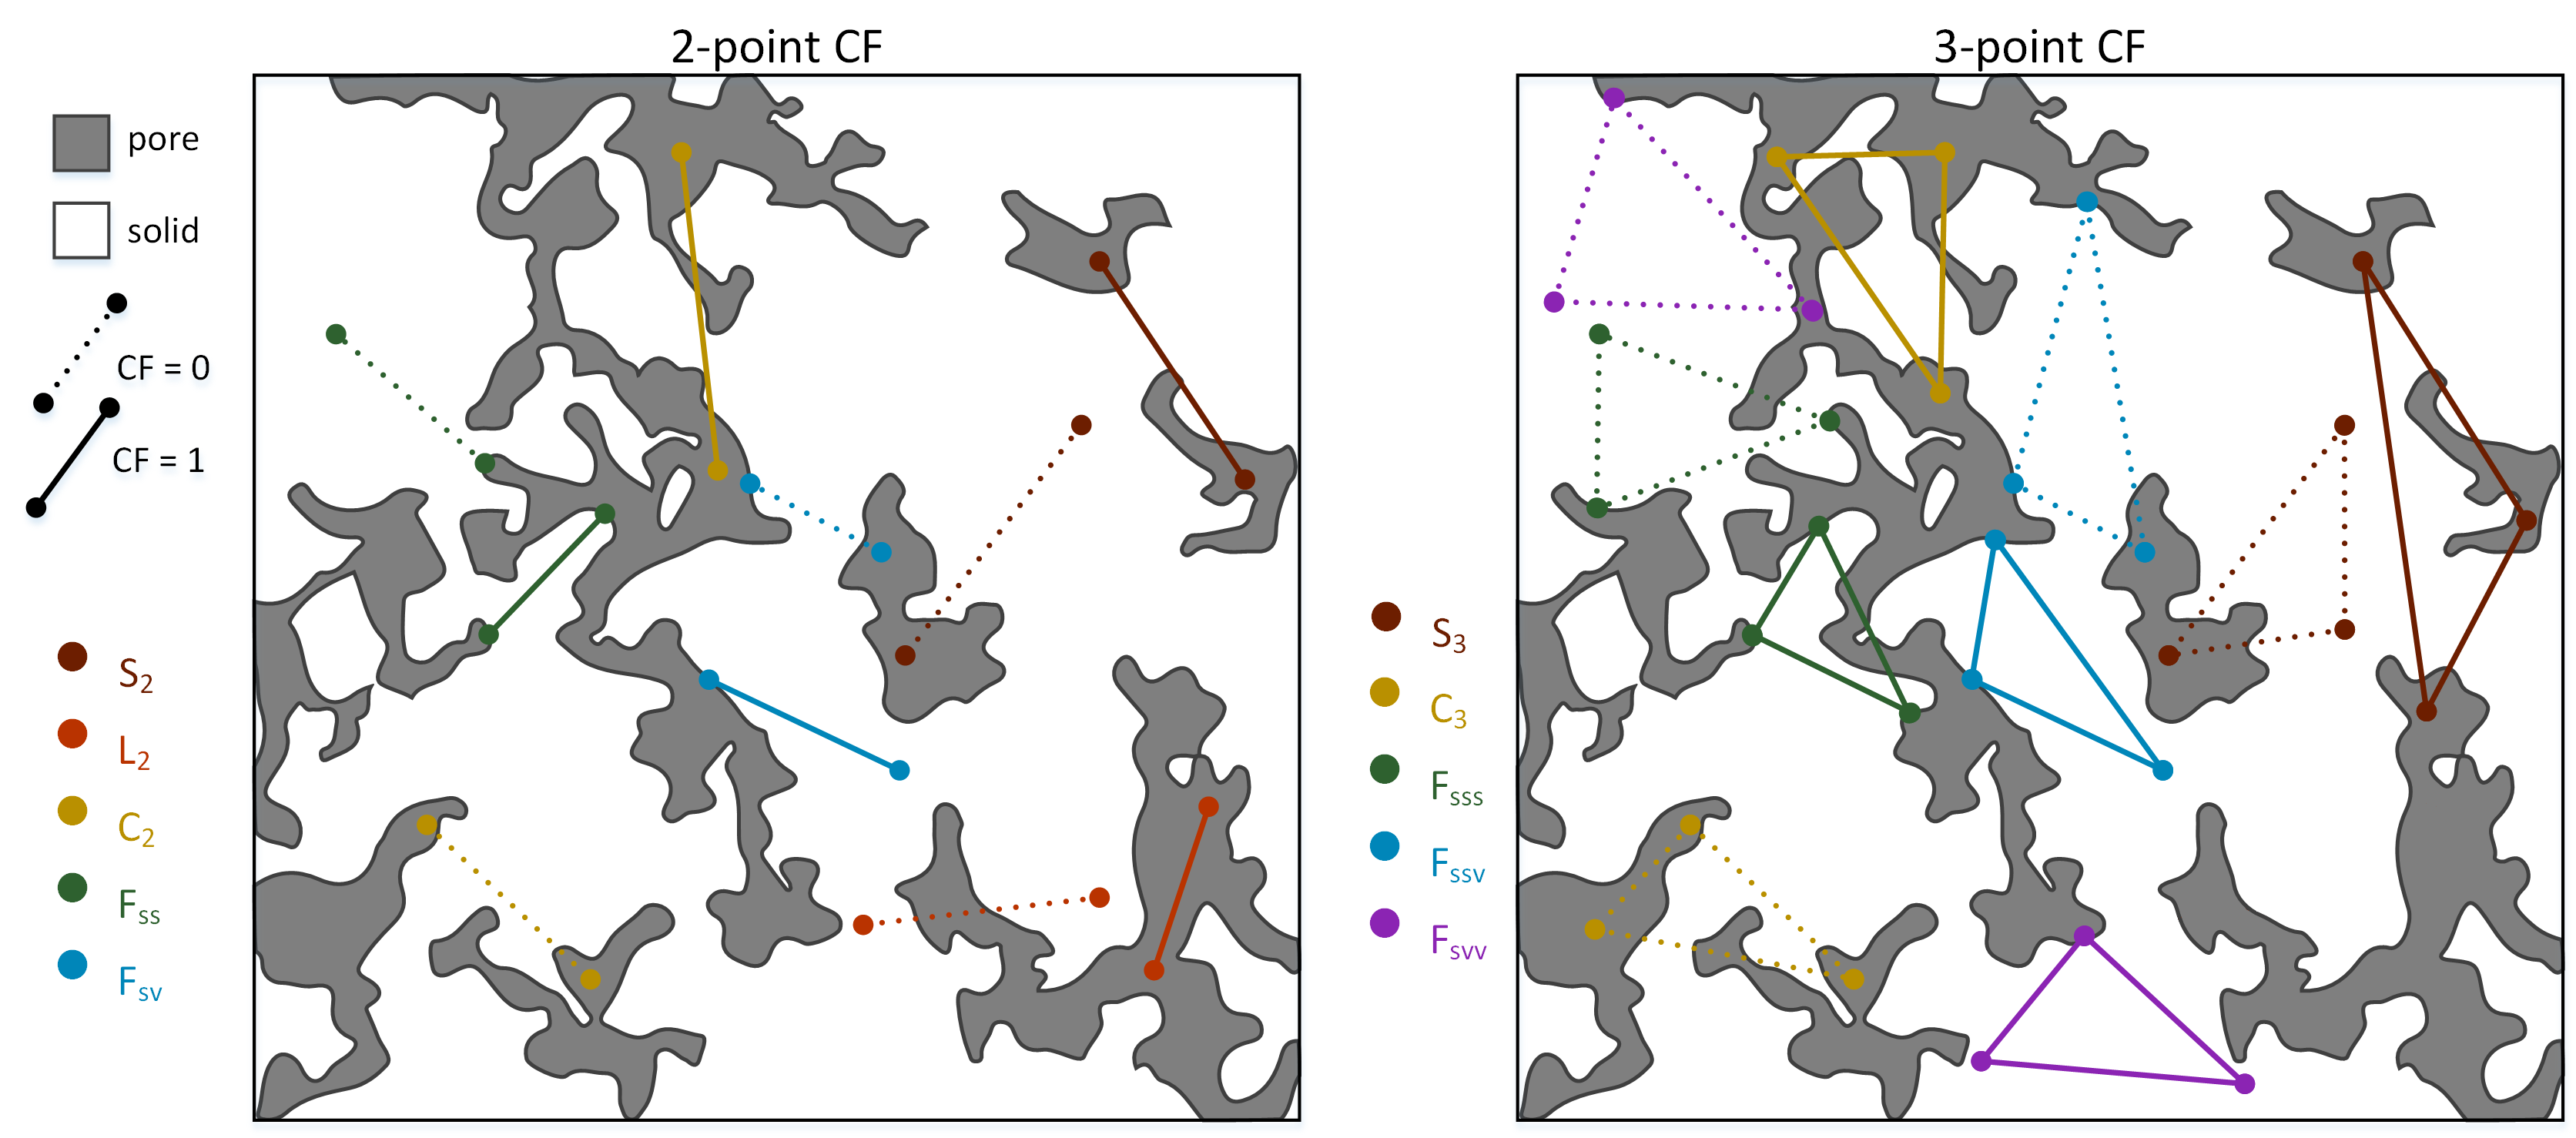
\includegraphics[width=0.8\linewidth]{images/3point.png}
  \caption[]{A schematic representation of a binary porous media (pores are
    shaded) with examples of CFs computations (all classic two- and three-point
    correlation functions are presented according to the legend on the left
    side). Computations take into account all possible configurations of a line
    segment which either make a contribution to the CF (conventionally shown as
    ``CF = 1'') or do not make a contribution (``CF = 0'').}
  \label{fig:3point-scheme}
\end{figure*}
The large portion of the research papers mentioned above
\cite{rozenbaum2014,karsanina2015,ledesma2018,derossi2019,portillo2018developing,
  takada2003three,hopkins2013stars,jiao2013,Torquato_book,roding2020predicting,
  KarsaninaEJSS,capek2009,gerke2019tensor,REVpaper,LavrukhinPRE,Adler_recon,Y-T,
  tahmasebiPRL,Euras2012,EPL2,karsaninaPRL,jiao2007,SciRep1,Havelka,Geoderma2018}
is based on so-called correlation functions (CFs). These functions define a
probability that some events are occurring withing the structure (with some
special cases of surface functions), for example, 2-point probability $S_2$
measures the probability that both ends of the line segment are within the same
phase, 2-point cluster function $C_2$ -- that both ends of the line segment are
within the same interconnected cluster of same phase, and lineal path $L_2$
measures the probability that the whole segment lies within the phase (see
\cref{fig:3point-scheme}). Compared to other descriptors, CFs possess a number
of features making them, in our opinion, a perfect candidate for universal
descriptor:
\begin{enumerate}
  \item They contain the majority of other metrics inside. For example, porosity
    is $S_2(0)$ (and at zero correlation length of the majority of correlation
    functions except for surface ones), surface area is represented by in the
    derivative at $S_2(0)$ \cite{debye1957scattering}. Connectivity is described by cluster
    functions $C_2$ or $C_3$. Pore-size distribution is related to pore-size
    function and partially by $L_2$ and $S_3$. Surface-void functions are
    interconnected with mean curvature and Euler characteristic
    \cite{ma2020generation}. Altogether, the classic set of correlation
    functions describes both the geometry and topology of the structure at hand;
  \item While the extent to which such classical set describes any arbitrary
    structure is not yet known, compared to other complex descriptors where are
    known pathways to assess the information content of correlation functions --
    there is a methodology for $S_2$ \cite{Gommes2} and approaches for other
    functions \cite{Degeneraty.045306,cherkasov2023towards};
  \item In addition to a possibility to compute correlation functions using
    images or other structural data, i.e., similar to all other descriptors,
    some CFs can be also determined experimentally
    \cite{debye1957scattering,barrall1992nmr,dietrich1995scattering,li2018accurate};
  \item Correlation functions can be scaled \cite{karsaninaPRL} or manipulated,
    for example, to add functions into a single one \cite{moctezuma2002};
  \item As opposed to scalar metrics such as porosity, surface area or Minkowski
    functionals, CFs can be computed in directions and describe anisotropic
    structures;
  \item Numerous rigorous bounds to obtain thermal, elastic, electromagnetic and
    transport properties are known, among which the most known (and least useful
    due to the impractically huge gap between the bounds) are Hashin-Strikman
    bounds \cite{hashin1963variational}. Other expressions based on integration
    of higher order $S_n$ are known and were found to be close to direct
    simulations
    \cite{brown1955solid,beran1965use,milton1981bounds,hlushkou2015effective};
  \item One can control both the size of the CFs-based descriptor and the
    information content via correlation length, number of functions in the set
    (including directions \cite{EPL2}), and by the order of functions (e.g., 2-
    and 3-point versions, or even more points).
\end{enumerate}
This list highlights that correlations functions are indeed possess necessary
properties so satisfy key criteria stated above.

However, while 2-point CFs are computed and used in multitude of studies, higher
order functions, for example, 3-point correlation functions are not that widely
used. The reason for this is straightforward -- 3-point correlation functions
are more involved and, thus, require much more computational resources to
assess. It has been shown that the amount of additional information content with
each increase in number of points $n$ decreases \cite{yao1993high,Gommes2}. The
trade-off between additional information and computational burden is still not
clear. Nonetheless, the computation of 3-point statistics is known to be
advantageous at least in the number of applications as related to cosmology,
astrophysics and turbulence patterns analysis as they can probe non-Gaussian
signatures in the distribution of matter and energy, which are not captured by their
2-point counterparts
\cite{TakadaJain,hopkins2013stars,gorbunova2016precessing,yoo2022non}.

In this contribution we continue our initiative to develop a simple, efficient
and open-source solution to compute all classical correlation functions on CPU
and GPU architectures -- \code{CorrelationFunctions.jl} \cite{CFsjlpaper}. Here
we build upon previous results in computations of higher order functions with
$n > 2$, most notably by Malmir et al. \cite{malmir2018}, and our aim is to
develop robust and computationally efficient methods. In addition, we also
considered the case of anisotropic structures and how to describe them with
3-point correlation functions similar to directional 2-point CFs
\cite{10.1063/1.4867611,EPL1}.

The paper is organized as follows: in \cref{sec:methods} we provide
mathematical background and describe methods for computation of 3-point
correlation functions. Verification of these methods along with some results for
real-world samples (sandstone, soil, etc.) is described in
\cref{sec:results}. Section \ref{sec:discussion} provides the discussion, a
comparison with other existing methods and summarizes possible directions for
future research.

\section{Methods}
\label{sec:methods}
\subsection{3-point correlation functions}
Let $A_1, A_2, \dots, A_n$ be pairwise disjoint subsets of a set
$A \subset \mathbb{R}^n$, where the index can be interpreted as a phase on the
image $A$. We introduce a family of indicator functions
$I_n(x) : A \rightarrow \{0,1\}$ defined as:
\begin{equation}
  I_n(x) = \left\{
  \begin{array}{ll}
    1 & \quad x \in A_n \\
    0 & \quad \text{otherwise}
  \end{array}
  \right.
\end{equation}

Now we can define the three-point correlation function
$S_3: \mathbb{R}^{2n} \rightarrow [0, 1]$:
\begin{equation}
  S_3^n(x_1, x_2) = \langle I_n(x) I_n(x + x_1) I_n(x + x_2) \rangle
\end{equation}
where $\langle \dots \rangle$ means average over all points in $A$. It can be
understood as the probability that all three vertices of a triangle
$(0, x_1, x_2)$ will appear in the subset $A_n$ when the triangle is randomly
thrown in $A$. When $A$ represent isotropic medium, $x_1$ and $x_2$ can be
replaced with three numbers $r_1 = |x_1|$, $r_2 = |x_2|$ and $r_3 = |x_2 - x_1|$
to get a function of three scalar arguments.

Another function closely related to the three-point correlation function is the
cluster function which can be defined as:
\begin{equation}
  C_3^n(x_1, x_2) = \sum_{k=1}^K \langle \tilde{I}_k(x) \tilde{I}_k(x + x_1)
  \tilde{I}_k(x + x_2) \rangle
\end{equation}
where $\tilde{I}_k$ is an indicator function for $k$-th cluster and $K$ is a
total number of clusters. A cluster is a subset of $A_n$ so that any two points
in this subset can be connected with a curve belonging to that subset.

By introducing a function $M_n(x) = |\nabla I_n(x)|$ which is a so-called interface
indicator function, we can define three additional
correlation functions -- these are the surface-surface-surface function
($F_{sss}$), surface-surface-void function ($F_{ssv}$) and surface-void-void
function ($F_{svv}$). They are defined as:
\begin{align}
  F_{sss}^n(x_1, x_2) &= \langle M_n(x) M_n(x + x_1) M_n(x + x_2) \rangle \\
  F_{ssv}^n(x_1, x_2) &= \langle M_n(x) M_v(x + x_1) I_v(x + x_2) \rangle \\
  F_{svv}^n(x_1, x_2) &= \langle M_n(x) I_v(x + x_1) I_v(x + x_2) \rangle
\end{align}
Here $I_v$ is an indicator function for the subset of the void phase
$A_v$. Unlike $S_3$ and $C_3$ functions, these functions do not have the meaning
of probability and have the units of measurement inversely proportional to
volume, surface and length, respectively (e.g., can be measured in $\mu m^{-3}$, $\mu m^{-2}$ and
$\mu m^{-1}$ or other convenient dimensionless units depending on the problem to be solved). 
These functions describe the interface of the subset $A_n$ and
its spatial configuration with respect to $A_v$.

\subsection{Computational algorithms}
Three-point correlation function $S_3$ can be computed either in spatial domain
or in frequency domain via the convolution theorem. Suppose that a finite
countable set $A$ is defined as a multidimensional array. A point $x$ belongs to
a subset $A_n$ if and only if $A[x] = n$. The simplest algorithm below
calculates $S_3$ pointwise in the spatial domain:
\begin{algorithmic}[1]
  \Procedure{$S_3$}{$A, n, x_1, x_2$}
  \State $A_n \gets I_n (A)$
  \Comment Apply $I_n$ to the input array elementwise.
  \State $A'_n \gets \mathfrak{S}_{x_1}(A_n)$
  \State $A''_n \gets \mathfrak{S}_{x_2}(A_n)$
  \State $T \gets A_n \cdot A'_n \cdot A''_n$
  \State \textbf{return} $Sum(T) / Norm(A, x_1, x_2)$
  \EndProcedure
\end{algorithmic}
In this algorithm the indicator function $I_n$ for the phase of interest $n$ is
applied to the input array $A$. Then the shift operator $\mathfrak{S}$ is used
to shift $A_n$ by vectors $x_1$ and $x_2$. Finally, the three arrays are
multiplied pointwise and a normalized sum of all elements of the product is
returned.

There are two common boundary conditions when applying $\mathfrak{S}$. The
first condition is to extend $A_n$ periodically (\cref{fig:s3-periodic}) when
accessing out-of-bounds array elements. In this case $\mathfrak{S}_z$ is a
circular shift operator:
\begin{equation}
  A[x] \leftarrow A[x+z \mod d]
\end{equation}
In this case $Norm(A, x_1, x_2)$ does not depend on $x_1$ and $x_2$ and
is equal to the total number of elements in $A$. The second condition is to
replace out-of-bound elements with zeros (so-called zero padding)
(\cref{fig:s3-zeros}). A formula for $Norm(A, x_1, x_2)$ in this case is in Appendix
\ref{sec:number-of-trials} and $\mathfrak{S}_z$ is defined as follows:
\begin{equation}
  A[x] \leftarrow \left\{
  \begin{array}{ll}
    A[x+z] & \quad \text{if $x+z$ is a correct index in $A$} \\
    0 & \quad \text{otherwise}
  \end{array}
  \right.
\end{equation}
\begin{figure*}[tp]
  \centering
  \subfigure[Periodic boundary conditions]{
    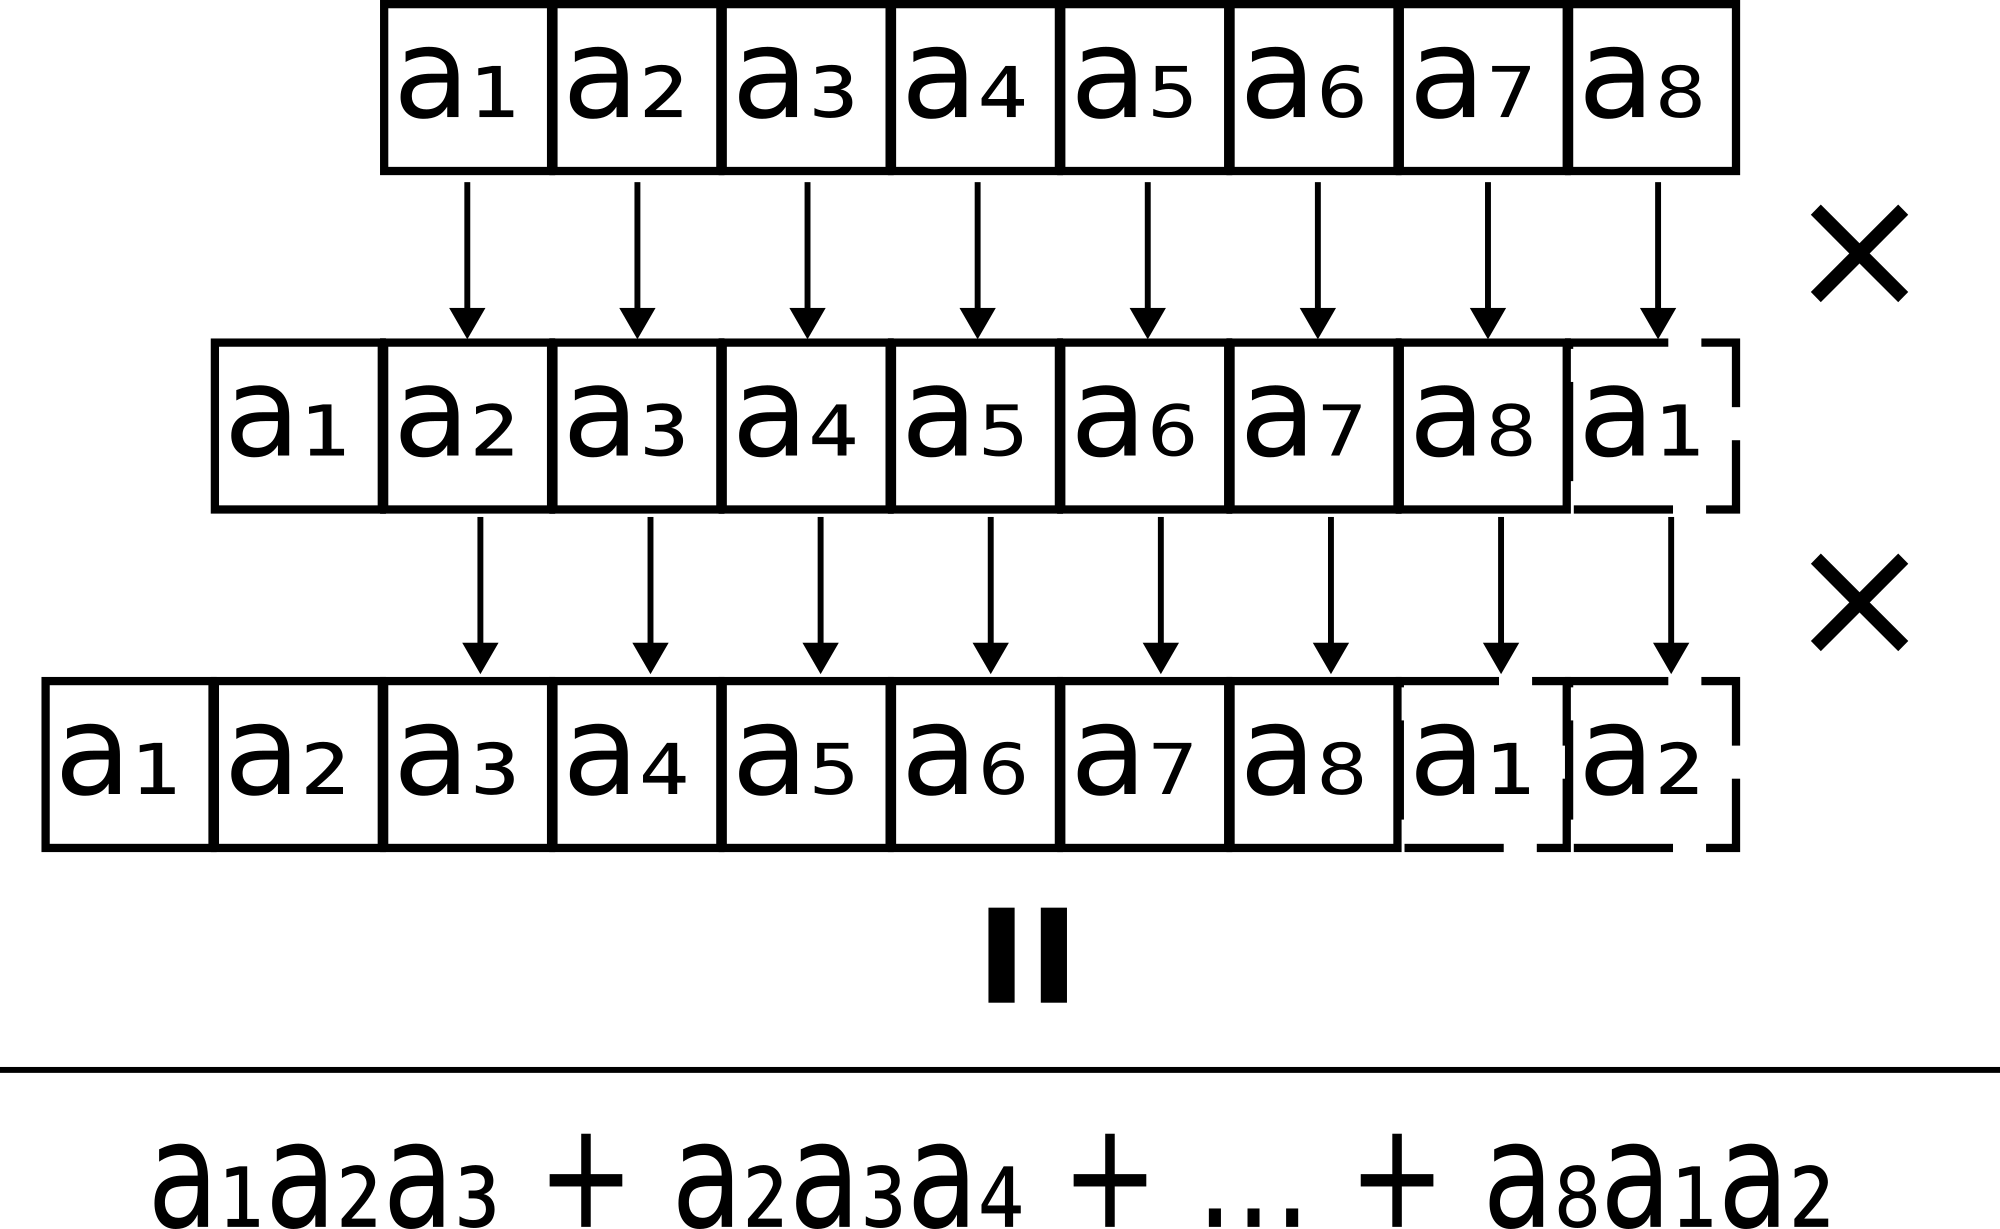
\includegraphics[width=0.4\linewidth]{images/periodic.png}
    \label{fig:s3-periodic}}
  \hfill
  \subfigure[Zero padding]{
    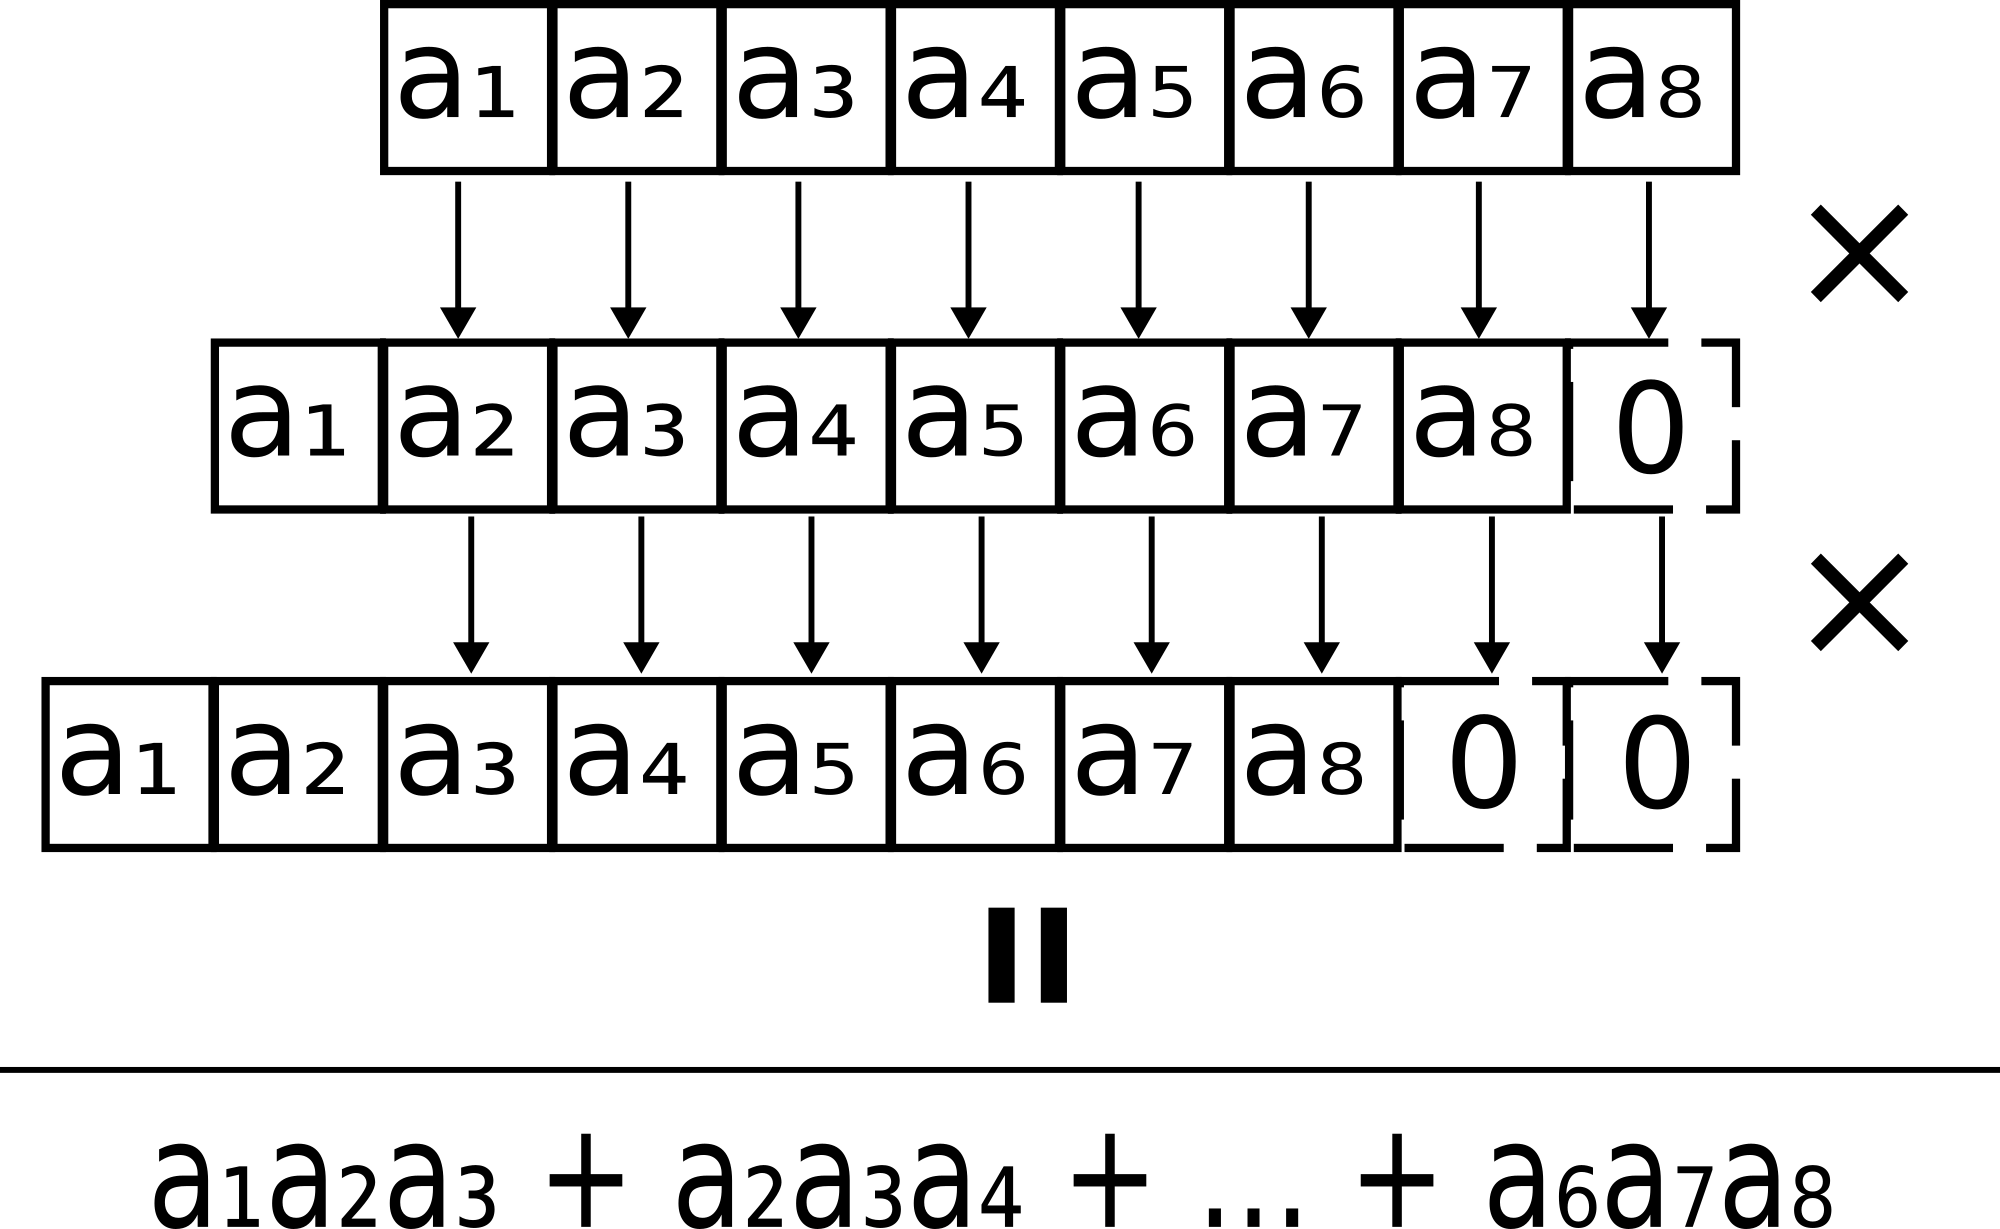
\includegraphics[width=0.4\linewidth]{images/zeros.png}
    \label{fig:s3-zeros}}
  \caption[]{Computation of unnormalized $S_3$ function at point $(1, 2)$ for
    one-dimensional sequence of length 8.}
  \label{fig:s3-computation}
\end{figure*}

The second approach is to compute the whole correlation map in the Fourier
domain. Suppose we have a function
$f: \mathbb{R} \rightarrow \mathbb{R}$. Triple correlation for this function is:
\begin{equation}
  g(t_1, t_2) = \int f(\tau) f(\tau + t_1) f(\tau + t_2) d \tau.
\end{equation}
We can use a well-known formula to compute Fourier image of $g$:
\begin{equation}
  \hat{g}(z_1, z_2) = \hat{f}(z_1) \hat{f}(z_2) \overline{\hat{f}(z_1 + z_2)}
\end{equation}
This algorithm has a better computational complexity compared with the previous
algorithms if the whole correlation map is needed ($O(n^2 \log n)$ vs
$O(n^3)$ where $n$ is a number of elements in the input array). The whole
correlation map, however, requires a lot of memory and is rarely
needed. Imagine, that the input array $A$ is of dimensions $500 \times 500$.
Then, considering that single precision floating point numbers are used,
$4 \cdot 2 \cdot 500^4 / 1000^3 = 500$ GB are needed to store Fourier image of
the map. Moreover, Fourier image of the whole map has to be computed even if only one
element of the map in spatial domain is required. The aforementioned limitations
render this approach impractical.

Our implementation fixes $x_1$ and $x_2$ to be parallel to one of the axes $X$,
$Y$ or $Z$ with restriction $x_1 \perp x_2$ (\cref{fig:pattern})
\cite{dimitrakopoulos2010high}. Thus, the output has dimensions $D_1 \times D_2$
where $D_1$ and $D_2$ are dimensions of the input array along selected
axes. Note that shift operators with such $x_1$ and $x_2$ represent a 3-point
function computed within a 3D domain, but along a predefined direction (see
below).
\begin{figure}[ht]
  \centering
  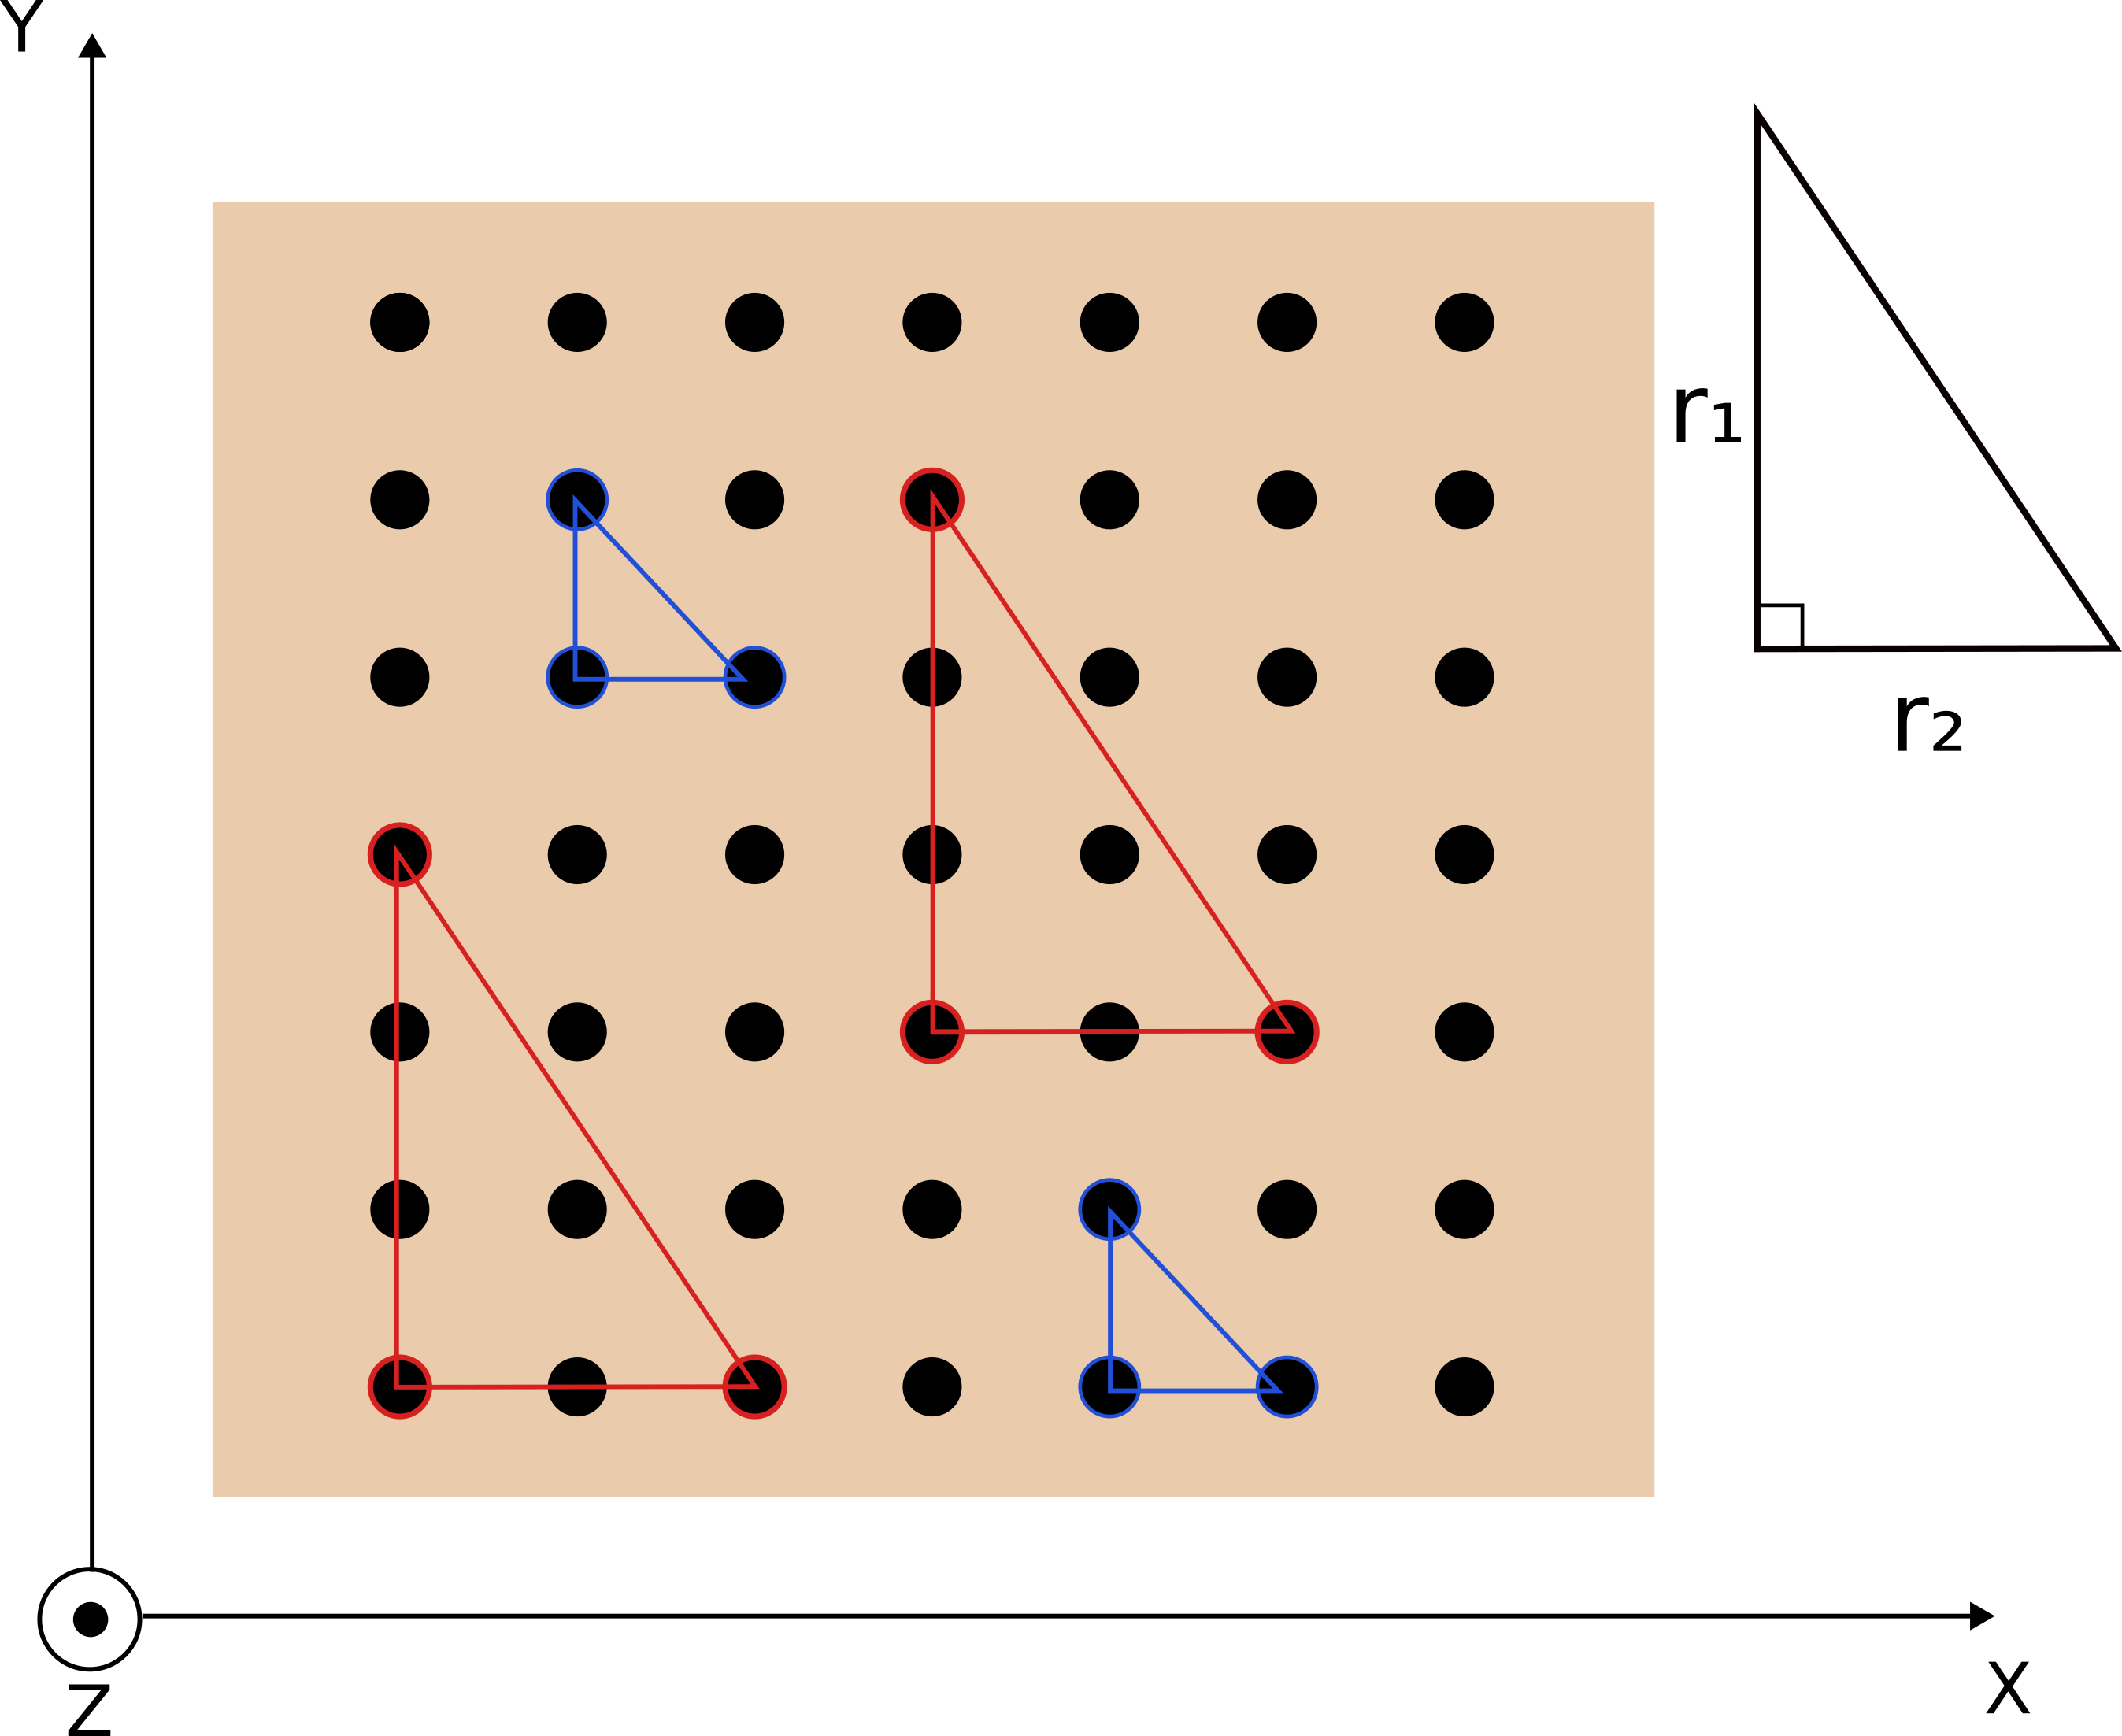
\includegraphics[width=0.5\linewidth]{images/pattern.png}
  \caption[]{The pattern used for calculation of $S_3$ function in our
    implementation.}
  \label{fig:pattern}
\end{figure}

Algorithms for three-point surface functions are the same as for $S_3$,
containing only small modifications. The main difference is that we need to
replace an indicator function $I_n$ with an edge detection operator $E_n$
(see Appendix \ref{sec:filter}). Then the algorithms are straightforward:
\begin{algorithmic}[1]
  \Procedure{$F_{sss}$}{$A, n, x_1, x_2$}
  \State $A_n \gets E_n (A)$
  \State $A'_n \gets \mathfrak{S}_{x_1}(A_n)$
  \State $A''_n \gets \mathfrak{S}_{x_2}(A_n)$
  \State $T \gets A_n \cdot A'_n \cdot A''_n$
  \State \textbf{return} $Sum(T) / Norm(A, x_1, x_2)$
  \EndProcedure

  \Procedure{$F_{ssv}$}{$A, n, x_1, x_2$}
  \State $A_n \gets E_n (A)$
  \State $A_{(void)} \gets I_{(void)} (A)$
  \State $A'_n \gets \mathfrak{S}_{x_1}(A_n)$
  \State $A'_{(void)} \gets \mathfrak{S}_{x_2}(A_{(void)})$
  \State $T \gets A_n \cdot A'_n \cdot A'_{(void)}$
  \State \textbf{return} $Sum(T) / Norm(A, x_1, x_2)$
  \EndProcedure

  \Procedure{$F_{svv}$}{$A, n, x_1, x_2$}
  \State $A_n \gets E_n (A)$
  \State $A_{(void)} \gets I_{(void)} (A)$
  \State $A'_{(void)} \gets \mathfrak{S}_{x_1}(A_{(void)})$
  \State $A''_{(void)} \gets \mathfrak{S}_{x_2}(A_{(void)})$
  \State $T \gets A_n \cdot A'_{(void)} \cdot A''_{(void)}$
  \State \textbf{return} $Sum(T) / Norm(A, x_1, x_2)$
  \EndProcedure
\end{algorithmic}

Input images must have appropriately high resolution for edge detection filter
to work correctly. A criterion for ``goodness'' of an image can be expressed
with $C_{\alpha}$ parameter \cite{samarin2023robust}. Let $\alpha \in [0, 1]$
and $f(x)$ be (band-limited) input image ($x \in \mathbb{R}^2$ or
$\mathbb{R}^3$). We define $C_\alpha$ as follows:
\begin{equation}
  \begin{aligned}
    f_0(x) &= f(x) - \langle f(x) \rangle \\
    C_\alpha &= \frac{\int_{-\alpha\omega}^{\alpha\omega} |\hat{f_0}(z)|^2
      dz}{\int_{-\omega}^{\omega} |\hat{f_0}(z)|^2 dz}
  \end{aligned}
\end{equation}
where $\hat{f_0}$ is a Fourier transform of $f_0$ and $\omega$ is a folding
frequency which depends only on resolution of the image. If a criterion
$C_{0.5} > 0.97$ holds then the image is suitable for application of
aforementioned algorithms for calculation of surface functions, otherwise
image's resolution can be improved with the help of interpolation prior to
computations \cite{samarin2023robust}.

To compute $C_3$ function we need to use a connected-component labeling
algorithm \cite{4728561,PhysRevB.14.3438} to label clusters. Then, again, a
slightly modified algorithm for $S_3$ is used to assess cluster function:
\begin{algorithmic}[1]
  \Procedure{$C_3$}{$A, n, x_1, x_2$}
  \State $A_n \gets I_n (A)$
  \State $C_n \gets \mathfrak{C}(A_n)$
  \State $C'_n \gets \mathfrak{S}_{x_1}(C_n)$
  \State $C''_n \gets \mathfrak{S}_{x_2}(C_n)$
  \State $T \gets C_n \odot C'_n \odot C''_n$
  \State \textbf{return} $Sum(T) / Norm(A, x_1, x_2)$
  \EndProcedure
\end{algorithmic}
Here $\mathfrak{C}$ is connected-component labeling operator and $\odot$ is
defined as follows:
\begin{equation}
  x \odot y = \left\{
  \begin{array}{ll}
    1 & \quad x = y \\
    0 & \quad \text{otherwise}.
  \end{array}
  \right.
\end{equation}

\subsection{Analysis of anisotropic media}
When an analyzed sample is anisotropic, i.e., it is stretched or oriented along
some specific direction, it may be beneficial to align one of the cathetus of
sampling triangle \cref{fig:pattern} with that direction. In this case the
anisotropy present in the sample will be properly captured by computed 3-point
correlation function.

To detect the direction of anisotropy we use an $N \times N$ (where $N$ is
dimensionality of the sample) covariance matrix for coordinates of points in the
phase of interest:
\begin{equation}
  C_{ij} = \sum_{x \in \left\{
    \begin{array}{l}
      \text{Coordinates of points} \\
      \text{in the phase of interset}
    \end{array}
    \right\}} (x_i - \overline{x_i})(x_j - \overline{x_j})
\end{equation}
and decompose $C$ as $T \Lambda T^{-1}$ where $T$ is a unitary matrix and
$\Lambda$ is diagonal. $T$ can always be made so that it defines a rotation (by
multiplication of one of the columns by $-1$ if needed, so that
$\det T = 1$). Application of this rotation to the sample makes the direction of
anisotropy parallel to one of the axes, so anisotropy can be better represented in
the correlation function \cref{fig:aniso}.
\begin{figure*}[!htp]
  \centering
  \begin{tabular}{ccc}
    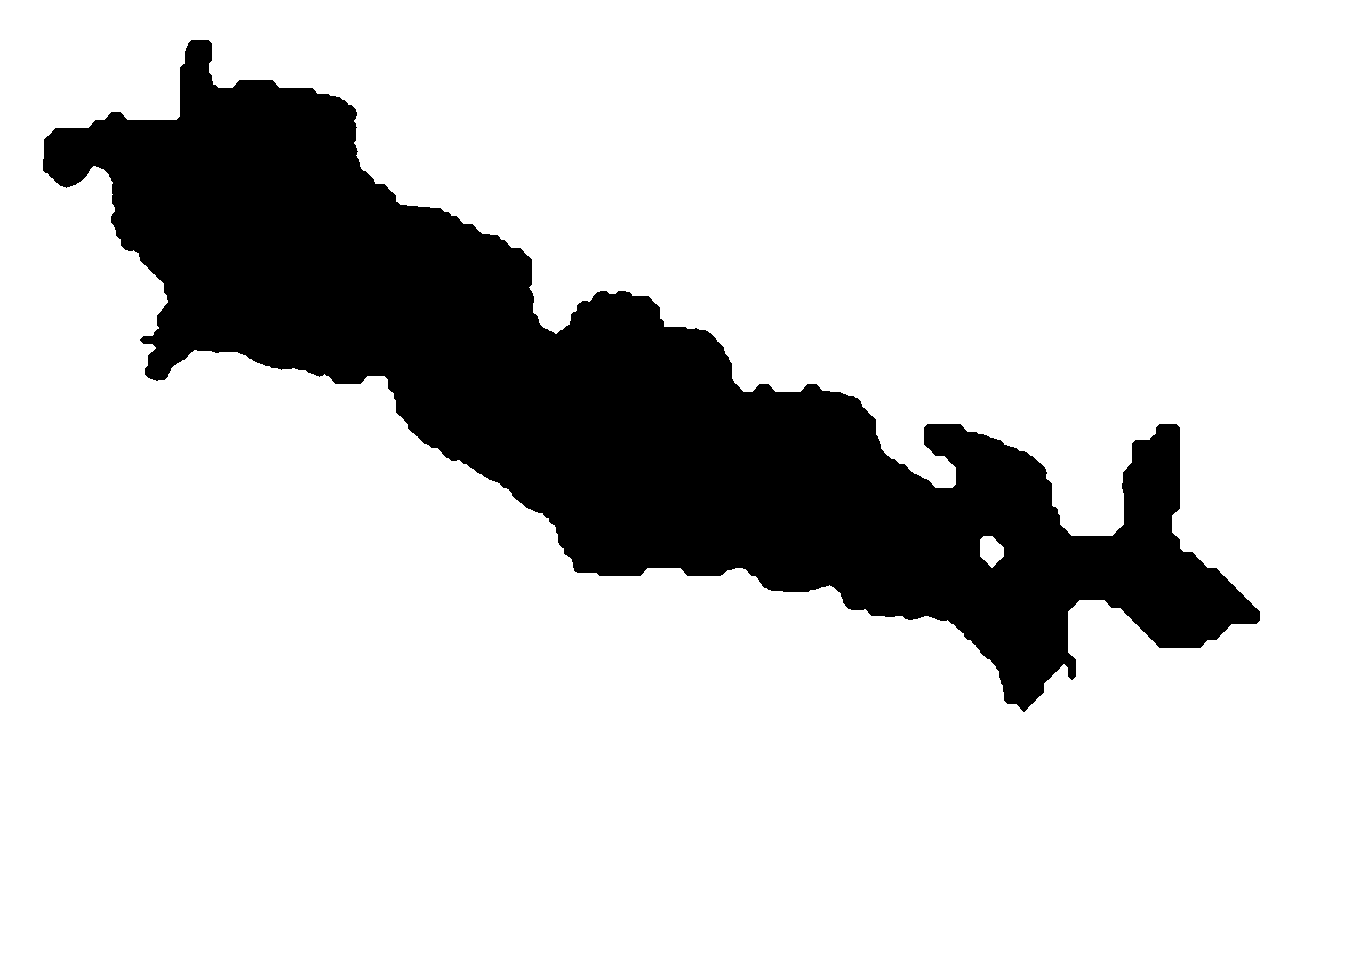
\includegraphics[width=0.3\linewidth, frame]{images/aniso.png} &
    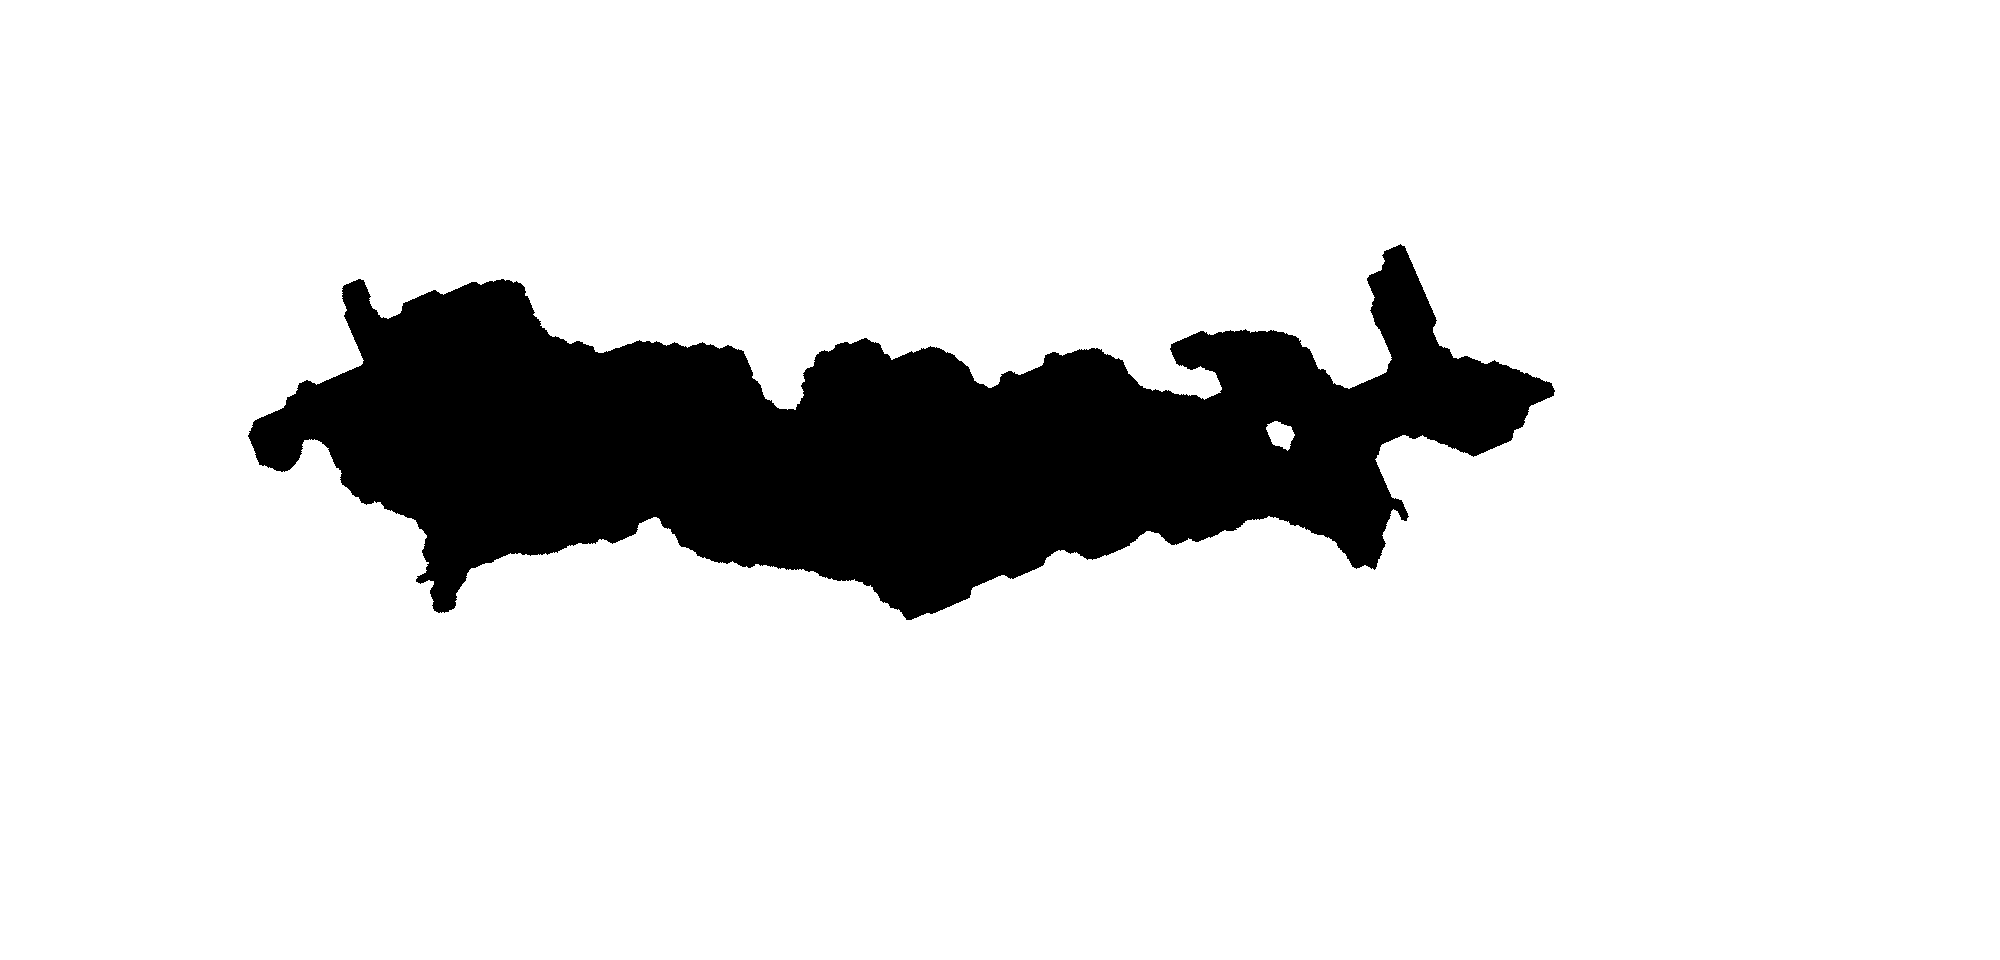
\includegraphics[width=0.3\linewidth, frame]{images/aniso-rot.png} & \\
    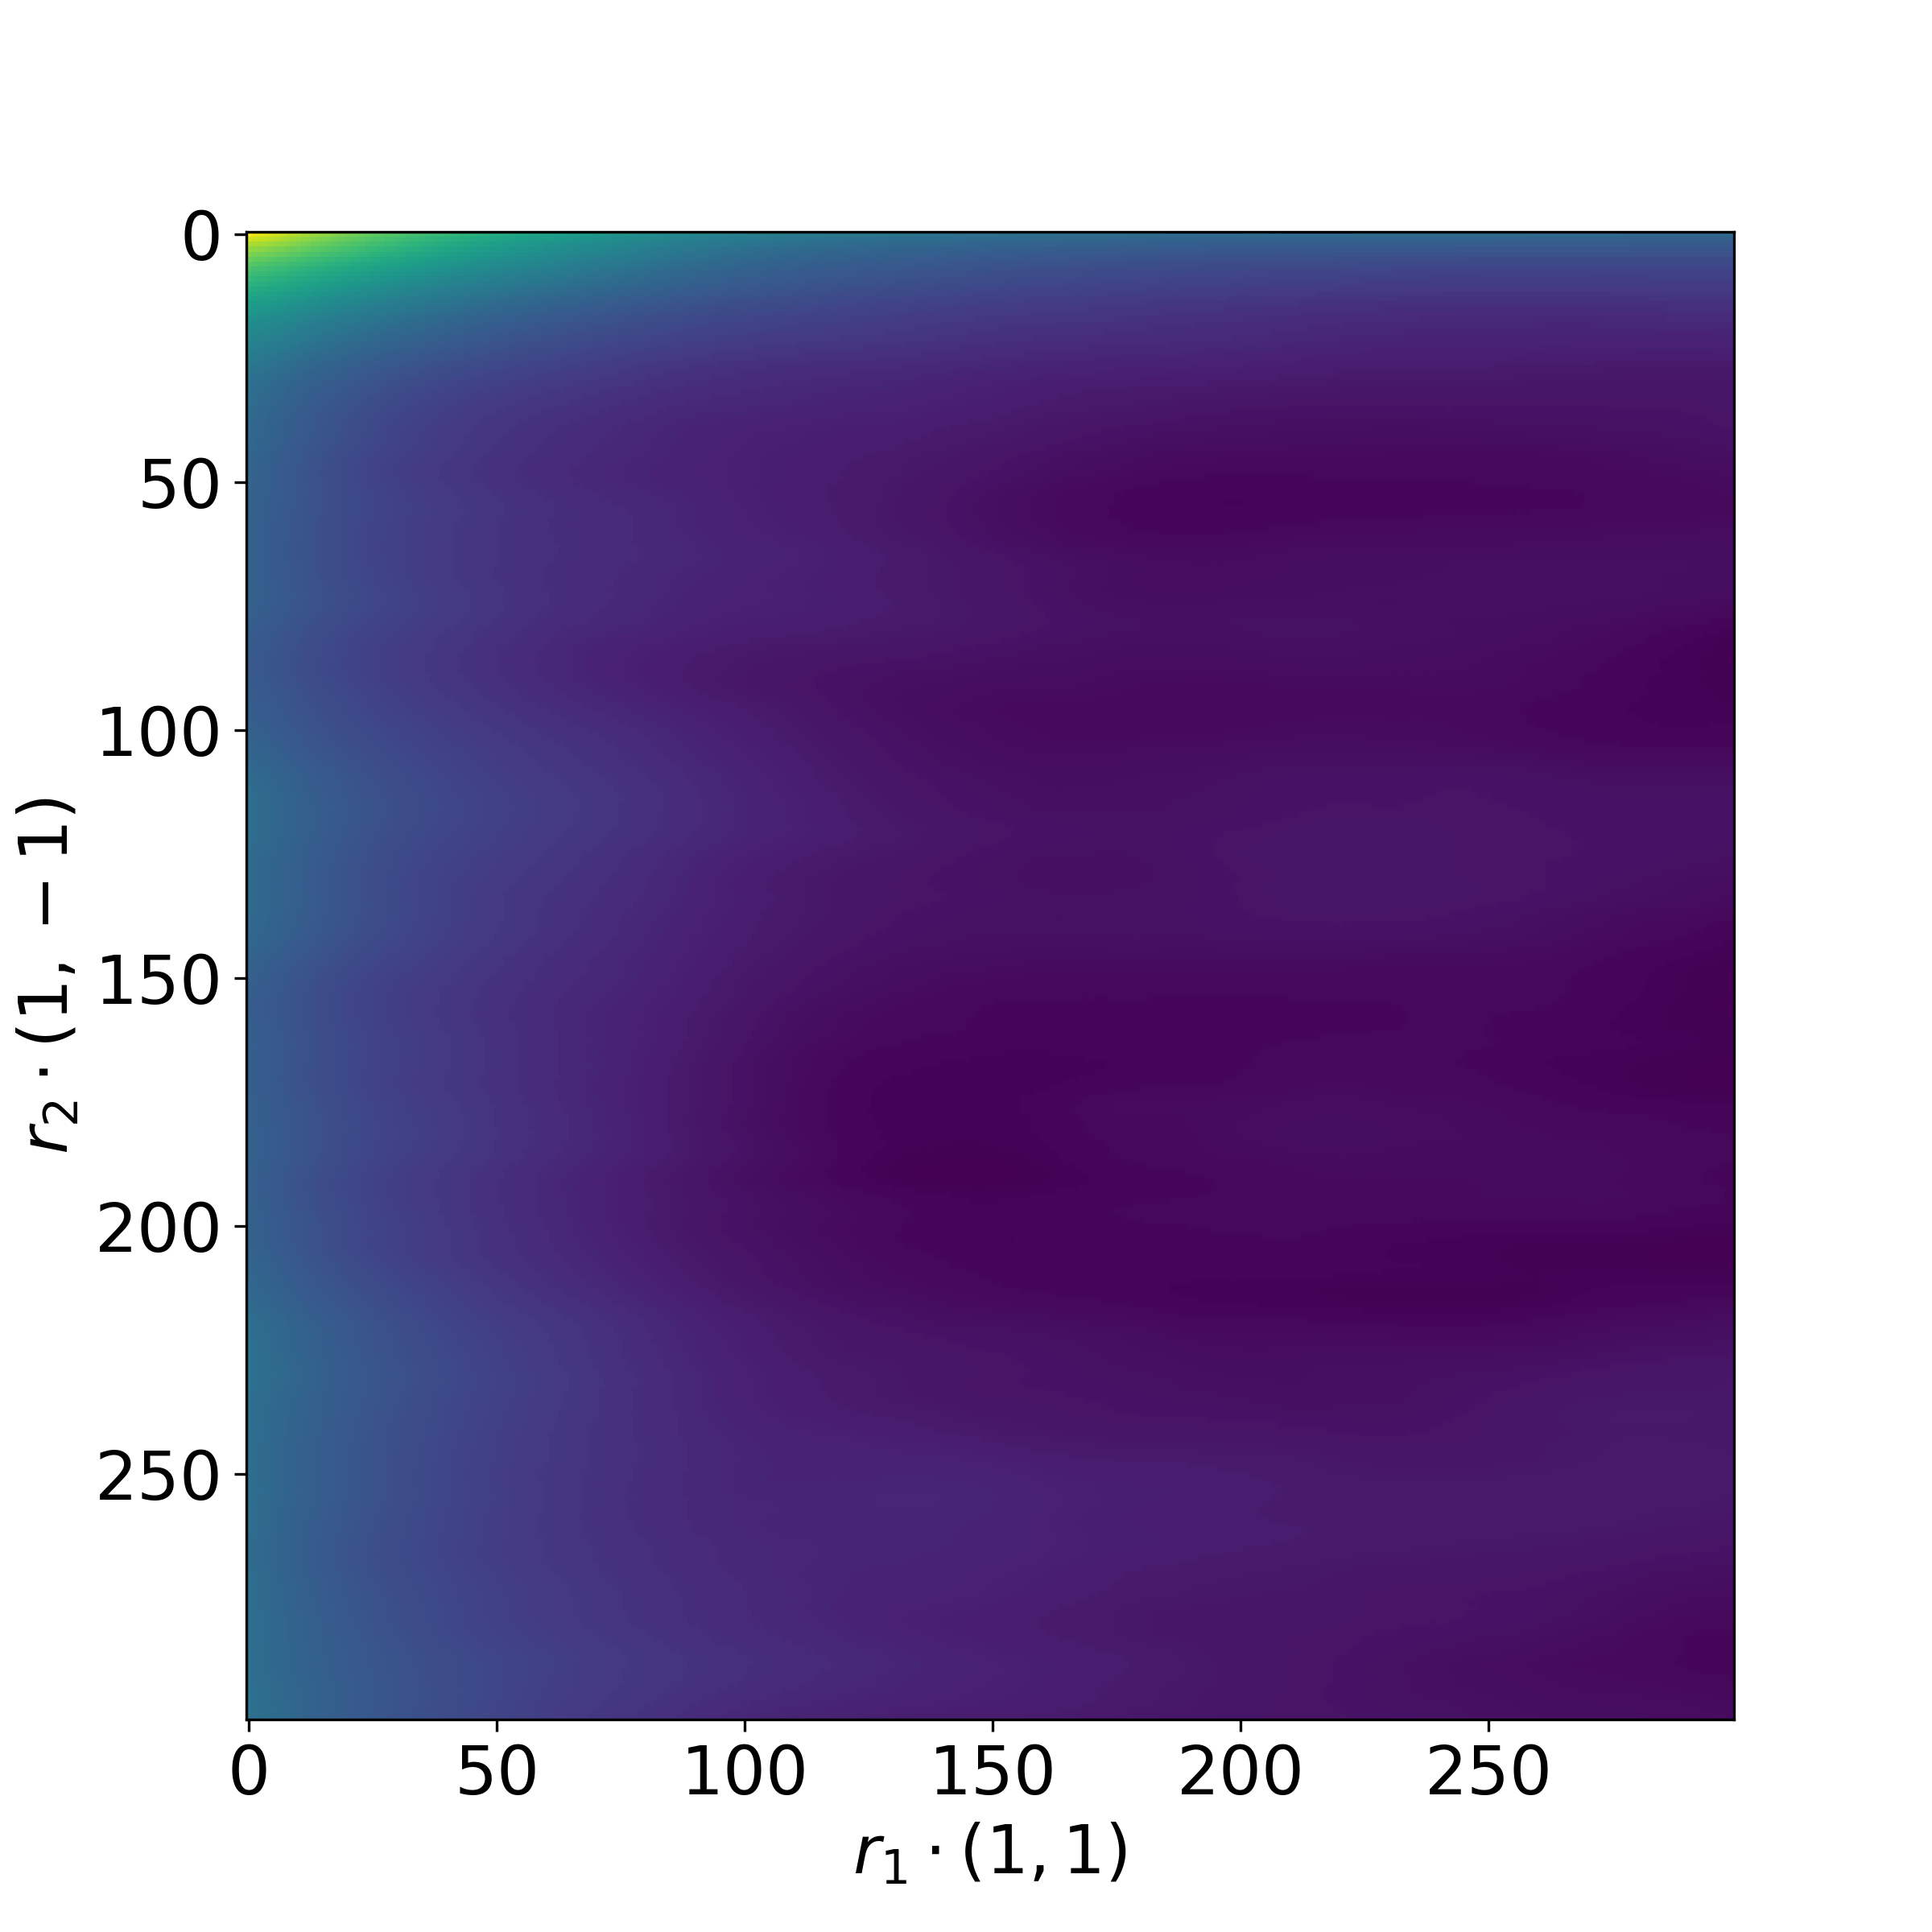
\includegraphics[width=0.3\linewidth]{images/aniso-s3.png} &
    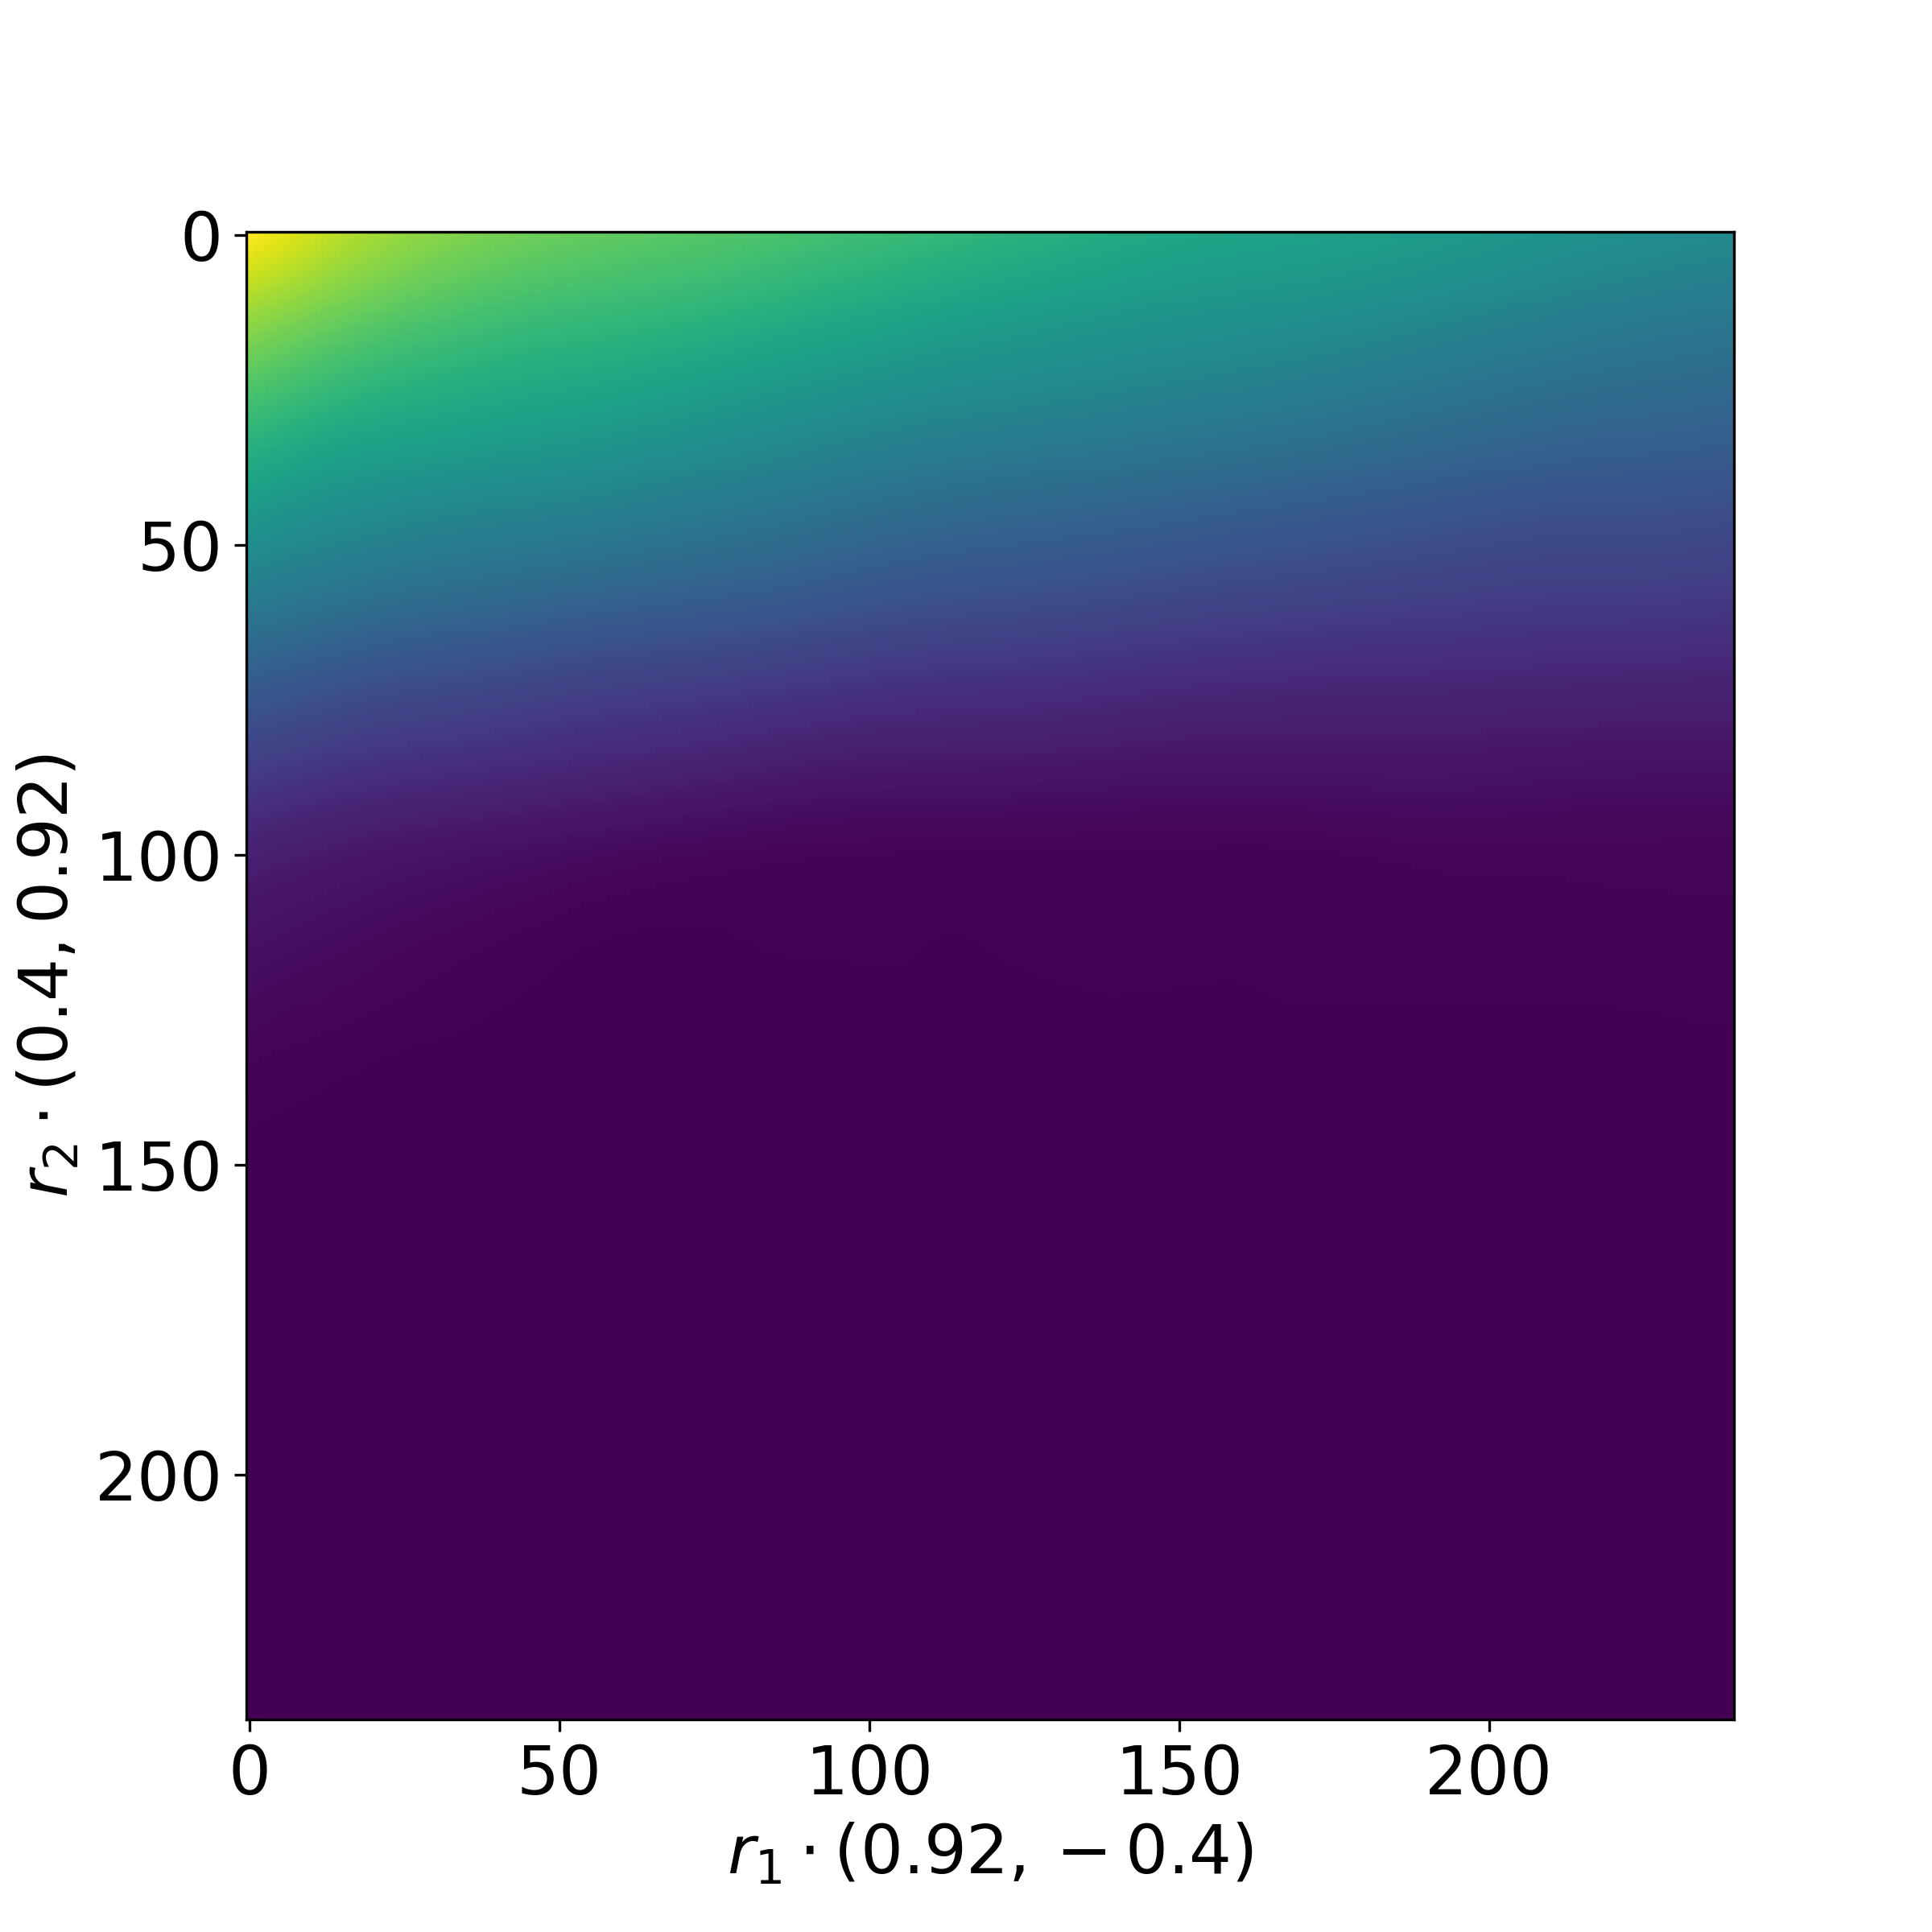
\includegraphics[width=0.3\linewidth]{images/aniso-rot-s3.png} &
    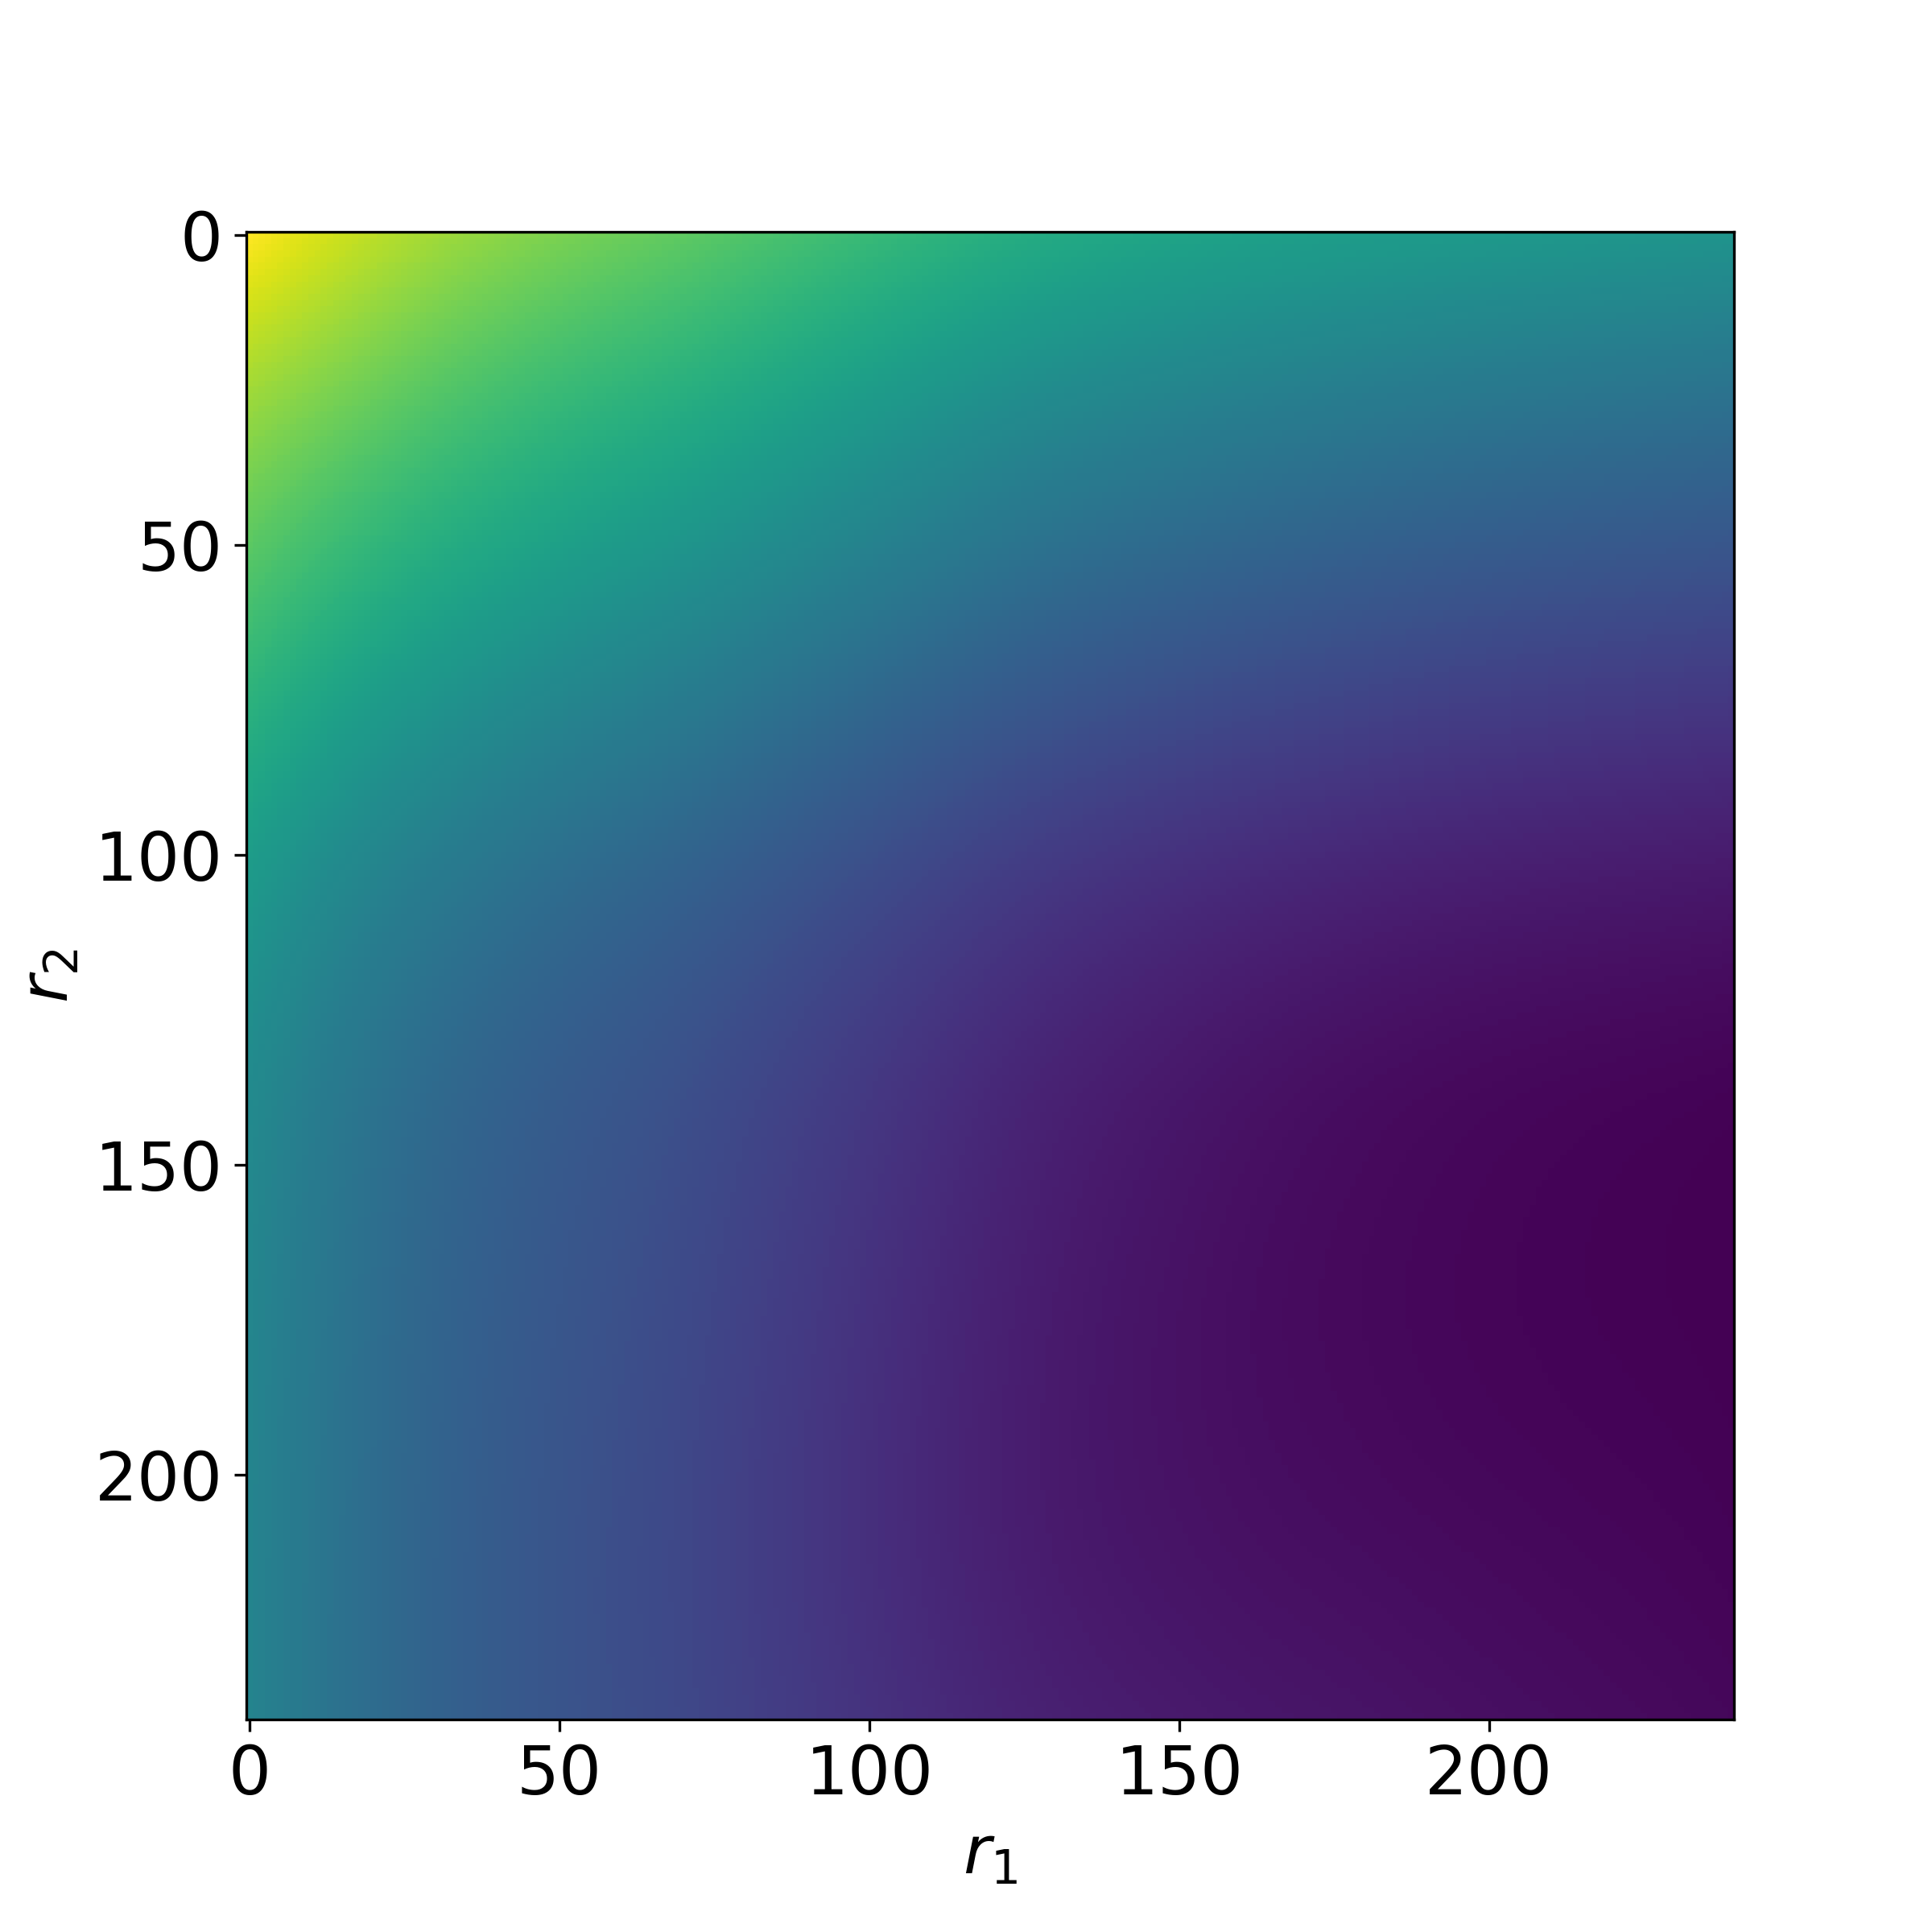
\includegraphics[width=0.3\linewidth]{images/aniso-avg-s3.png} \\
  \end{tabular}
  \caption{Behaviour of our algorithm for calculation of the $S_3$ function
    when dealing with highly anisotropic media. The pattern \cref{fig:pattern}
    which we use in our algorithm is most sensitive to anisotropy which is
    directed along one of the axes. \\
    From top down, left to right: an original image of an anisotropic pore; a
    rotated image of the pore, so it is elongated along the axis; $S_3$ function
    for the original pore; $S_3$ function for the rotated pore with a vector
    $(0.92, -0.4)$ being a direction of elongation of the pore; $S_3$ function
    averaged across rotations similar to the algorithm described in
    \cite{berryman1988,SMITH1988176,malmir2018}.}
  \label{fig:aniso}
\end{figure*}

\subsection{Directional and averaged computations}
When a sample is known to be isotropic, the correlation function may be
calculated multiple times, each time applying a random rotation of the sample,
and then averaged across rotations to gather more statistics. This process is
illustrated on \cref{fig:workflow}. This way we obtain similar results to
sampling procedures used in \cite{berryman1988,SMITH1988176,malmir2018}.

Another approach is to fix a number of directions, for example, orthogonal and
diagonal ones \cite{EPL1,EPL2,CFsjlpaper}. In other words, the sample is rotated
with periodic boundary conditions to orient along predefined directions. After
each rotation we compute correlation functions as described above and obtain a
number of matrices $D_1 \times D_2$ that are then stacked to represent 3-point
correlation functions computed in directions \cref{fig:workflow}.

To summarize, \code{CorrelationFunctions.jl} allows to compute 3-point
correlation functions averaged in all directions (by randomly rotating the
sample), along predefined number of directions (e.g., orthogonal and diagonal by
rotation in these directions) or along the direction of major anisotropy (that
can be determined using \code{$detect\_anisotropy$} function).  Full correlation
map for 3-point functions is impractical due its huge size and is not
implemented.

\begin{figure*}[tp]
  \centering
  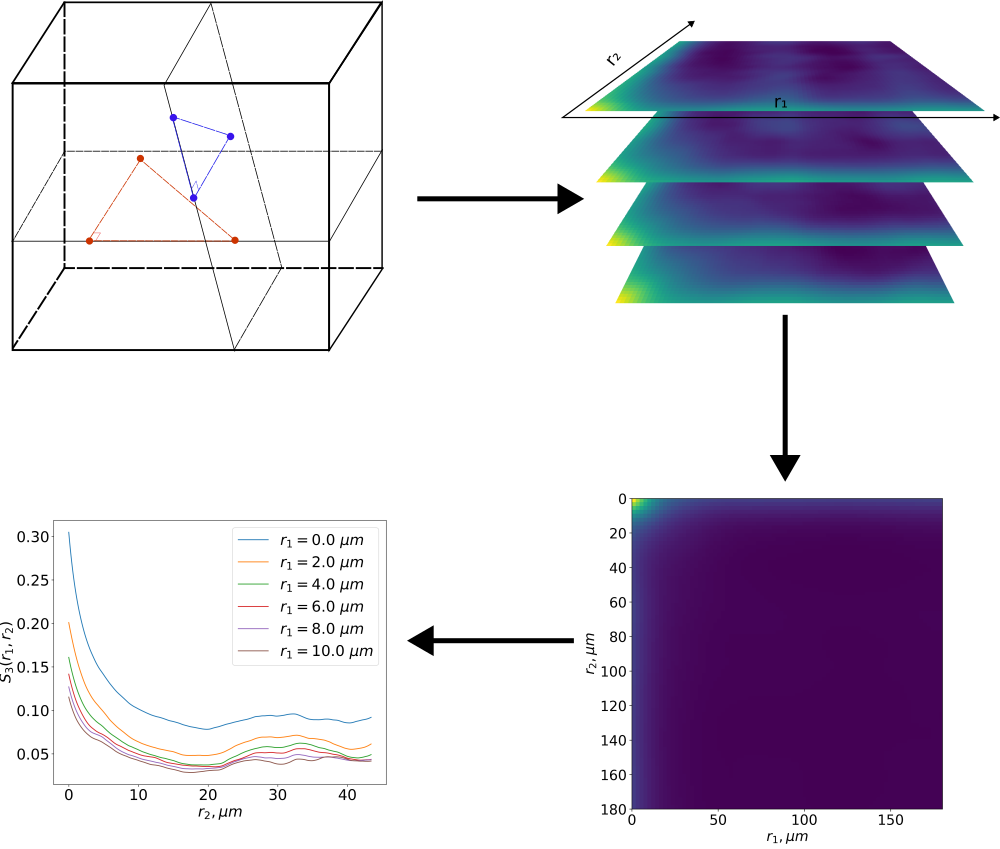
\includegraphics[width=0.6\linewidth]{images/workflow.png}
  \caption[]{A possible workflow for computation of correlation functions
    (clockwise from top left to bottom right ): 1.~rotating a sample in random
    directions (which is equivalent to rotating the sampling pattern),
    2.~calculating the correlation function for each direction, 3.~avegaring
    results across rotations, 4.~representing the result as a family of 2D
    plots. \highlight{Show "random rotation" at the slice, "Stack of directional
      functions" on the right-upper.}}
  \label{fig:workflow}
\end{figure*}

\section{Results}
\label{sec:results}
\subsection{Verification}
To verify correctness of computation of $S_3$ and $C_3$ functions we use the
following simple relations:
\begin{align}
  S_3^n (x, 0) = S_3^n (0, x) &= S_2^n(x) \\
  C_3^n (x, 0) = C_3^n (0, x) &= C_2^n(x) \\
  \lim_{\substack{x_1 \to \infty \\ x_2 \to \infty}} S_3^n (x_1, x_2) &= \phi_n^3
\end{align}
Here $\phi_n$ is a fraction of phase $n$ in $A$.

There are only few sets for which analytic expressions for $S_2$ are known. One
of those is a set consisting of overlapping balls with a fixed radius $R$ and
centers generated with Poisson process with parameter $\lambda$. In this case
the expression for $S_2$ is the following:
\begin{equation}
  \begin{aligned}
    S_2(r, R) &= \exp(-\frac{4}{3}\pi\lambda R^3 f(r, R)) \\
    f(r, R) &= \left\{
    \begin{array}{ll}
      1 + \frac{3}{4} \frac{r}{R} - \frac{1}{16} (\frac{r}{R})^3 & \quad r < 2R \\
      2 & \quad \text{otherwise}.
    \end{array}
    \right.
  \end{aligned}
  \label{eq:s2-balls}
\end{equation}

On \cref{fig:balls} there is an intersection of such a set with $R = 0.02$ and
$\lambda=5000$ within a cube $[0, 1]^3$. Because $R \ll 1$, we can use
\cref{eq:s2-balls} to verify our computations -- this is exactly what we present on
\cref{fig:balls-s3-comparison}.
\begin{figure*}[tp]
  \centering
  \subfigure[Realization of overlapping balls]{
    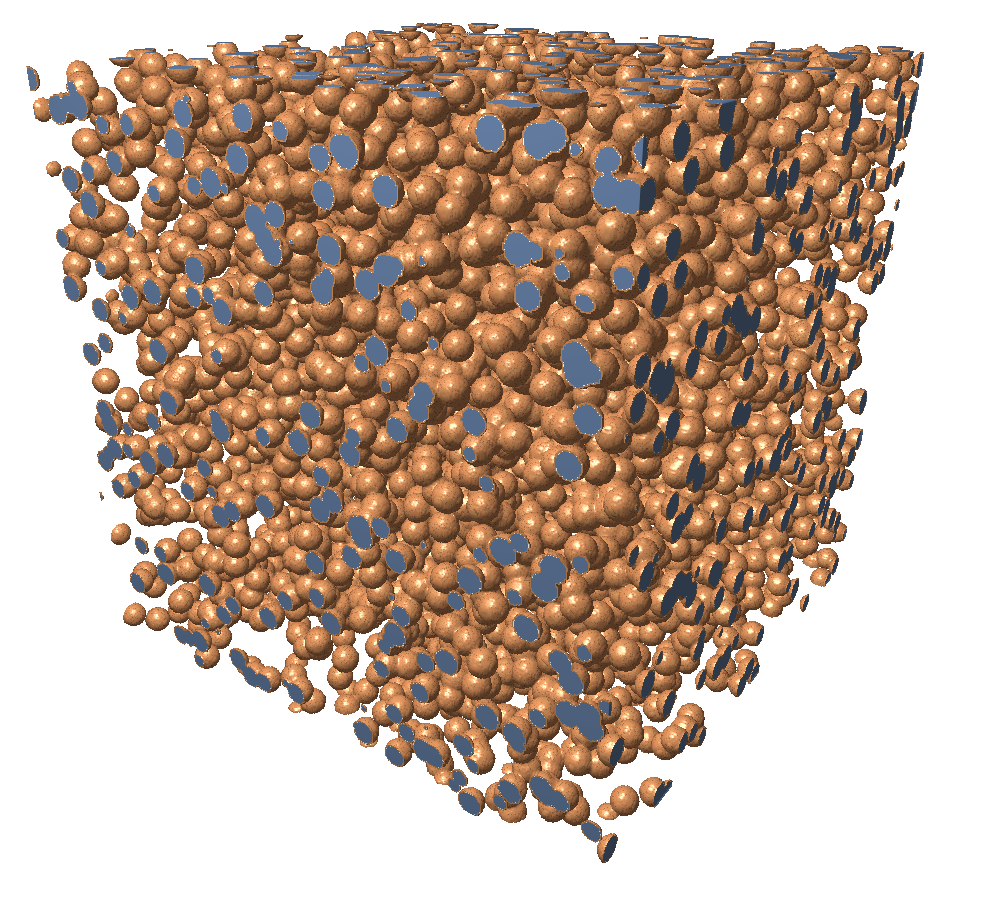
\includegraphics[width=0.4\linewidth]{images/balls.png}
    \label{fig:balls}}
  \hfill
  \subfigure[A plot of $S_3(0, r)$ computed with our algorithm and theoretical
    formula.]{
    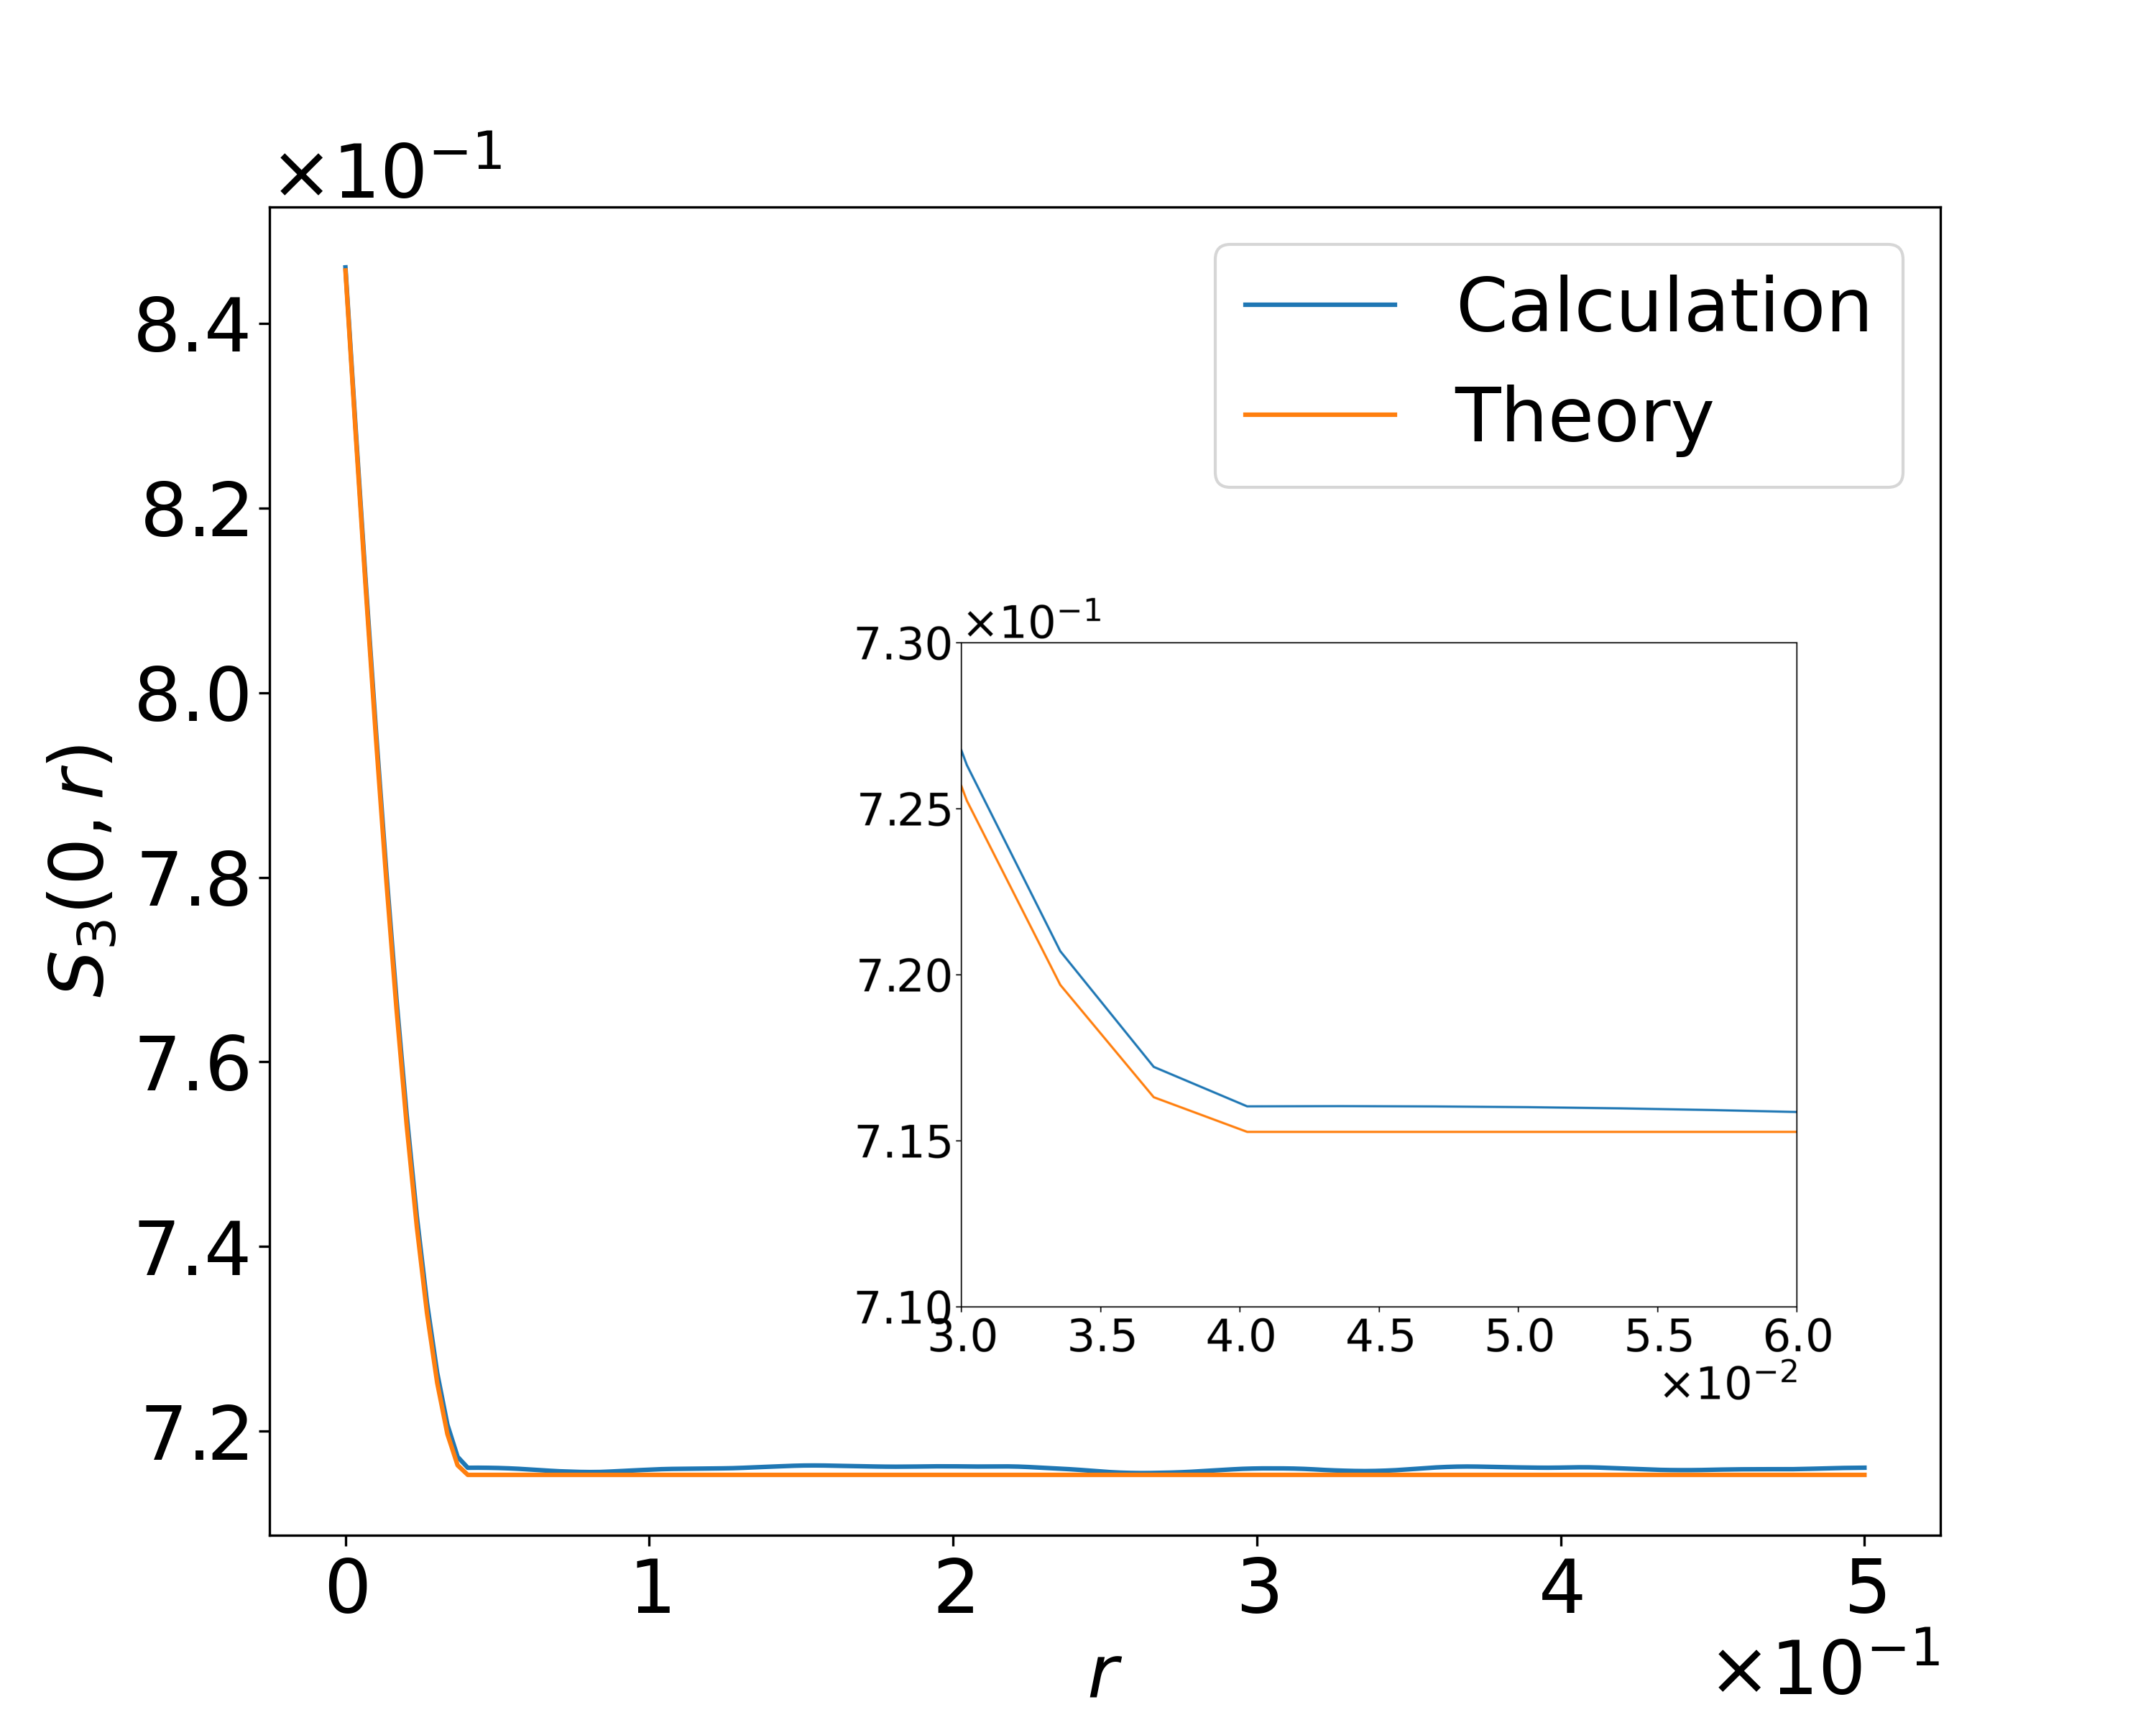
\includegraphics[width=0.4\linewidth]{images/balls-s3.png}
    \label{fig:balls-s3-comparison}}
  \caption[]{A comparison of calculated and theoretical values of $S_3$ function
    for overlapping balls.}
  \label{fig:s3-verification}
\end{figure*}

To test $F_{sss}$ function we use a recently developed approach which computes
that function for sets defined by inequality $f(x) \le T$, $x \in \mathbb{R}^3$
with help of automatic differentiation \cite{postnicov20232}. We choose $f$ as:
\begin{equation}
  f(x, y, z) = y^2 + z^2 - a x^2 (b^2 - x^2)
\end{equation}
and parameters $a = 10$, $b = 0.45$, $T = 10^{-2}$, so inequation
$f(x, y, z) \le T$ gives us a dumbbell-like object (\cref{fig:sss-dumbbell}).

The test is performed by firstly evaluating the inequation in a cube
$[-1, 1]^3$ and obtaining precise values of $F_{sss}$ and secondly computing
$F_{sss}$ with our algorithm, giving a discretized volume of $400^3$
voxels as the input. For ease of comparison, $F_{sss}$ function is evaluated within $XY$
plane. Pointwise relative error of $F_{sss}$ is on
\cref{fig:sss-dumbbell-error}. Maximal relative error in the area distanced
farther than 0.1 (20 pixels) from curves of discontinuity (see
\cref{fig:sss-dumbbell-precise}) is no more than 20\%.
\begin{figure*}[tp]
  \centering
  \subfigure[The dumbbell-like object used in testing of $F_{sss}$ computation]{
    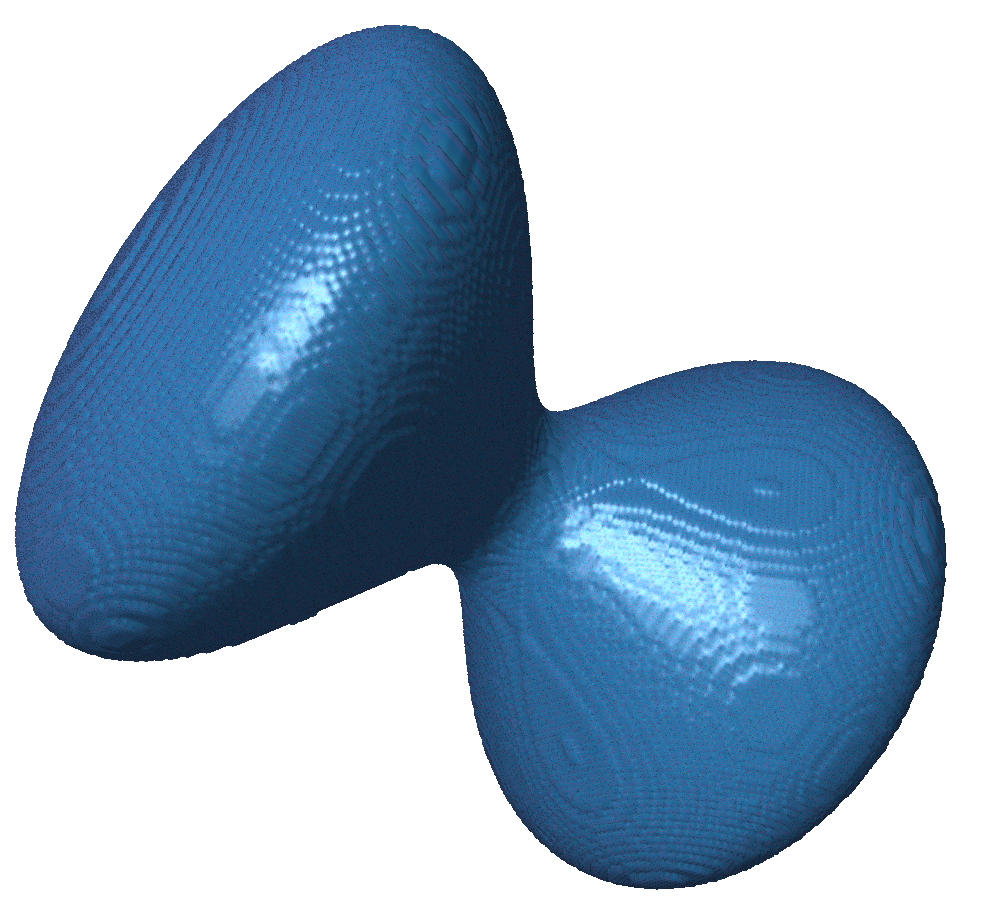
\includegraphics[width=0.4\linewidth]{images/dumbbell.png}
    \label{fig:sss-dumbbell}}
  \hfill
  \subfigure[Relative error of computation]{
    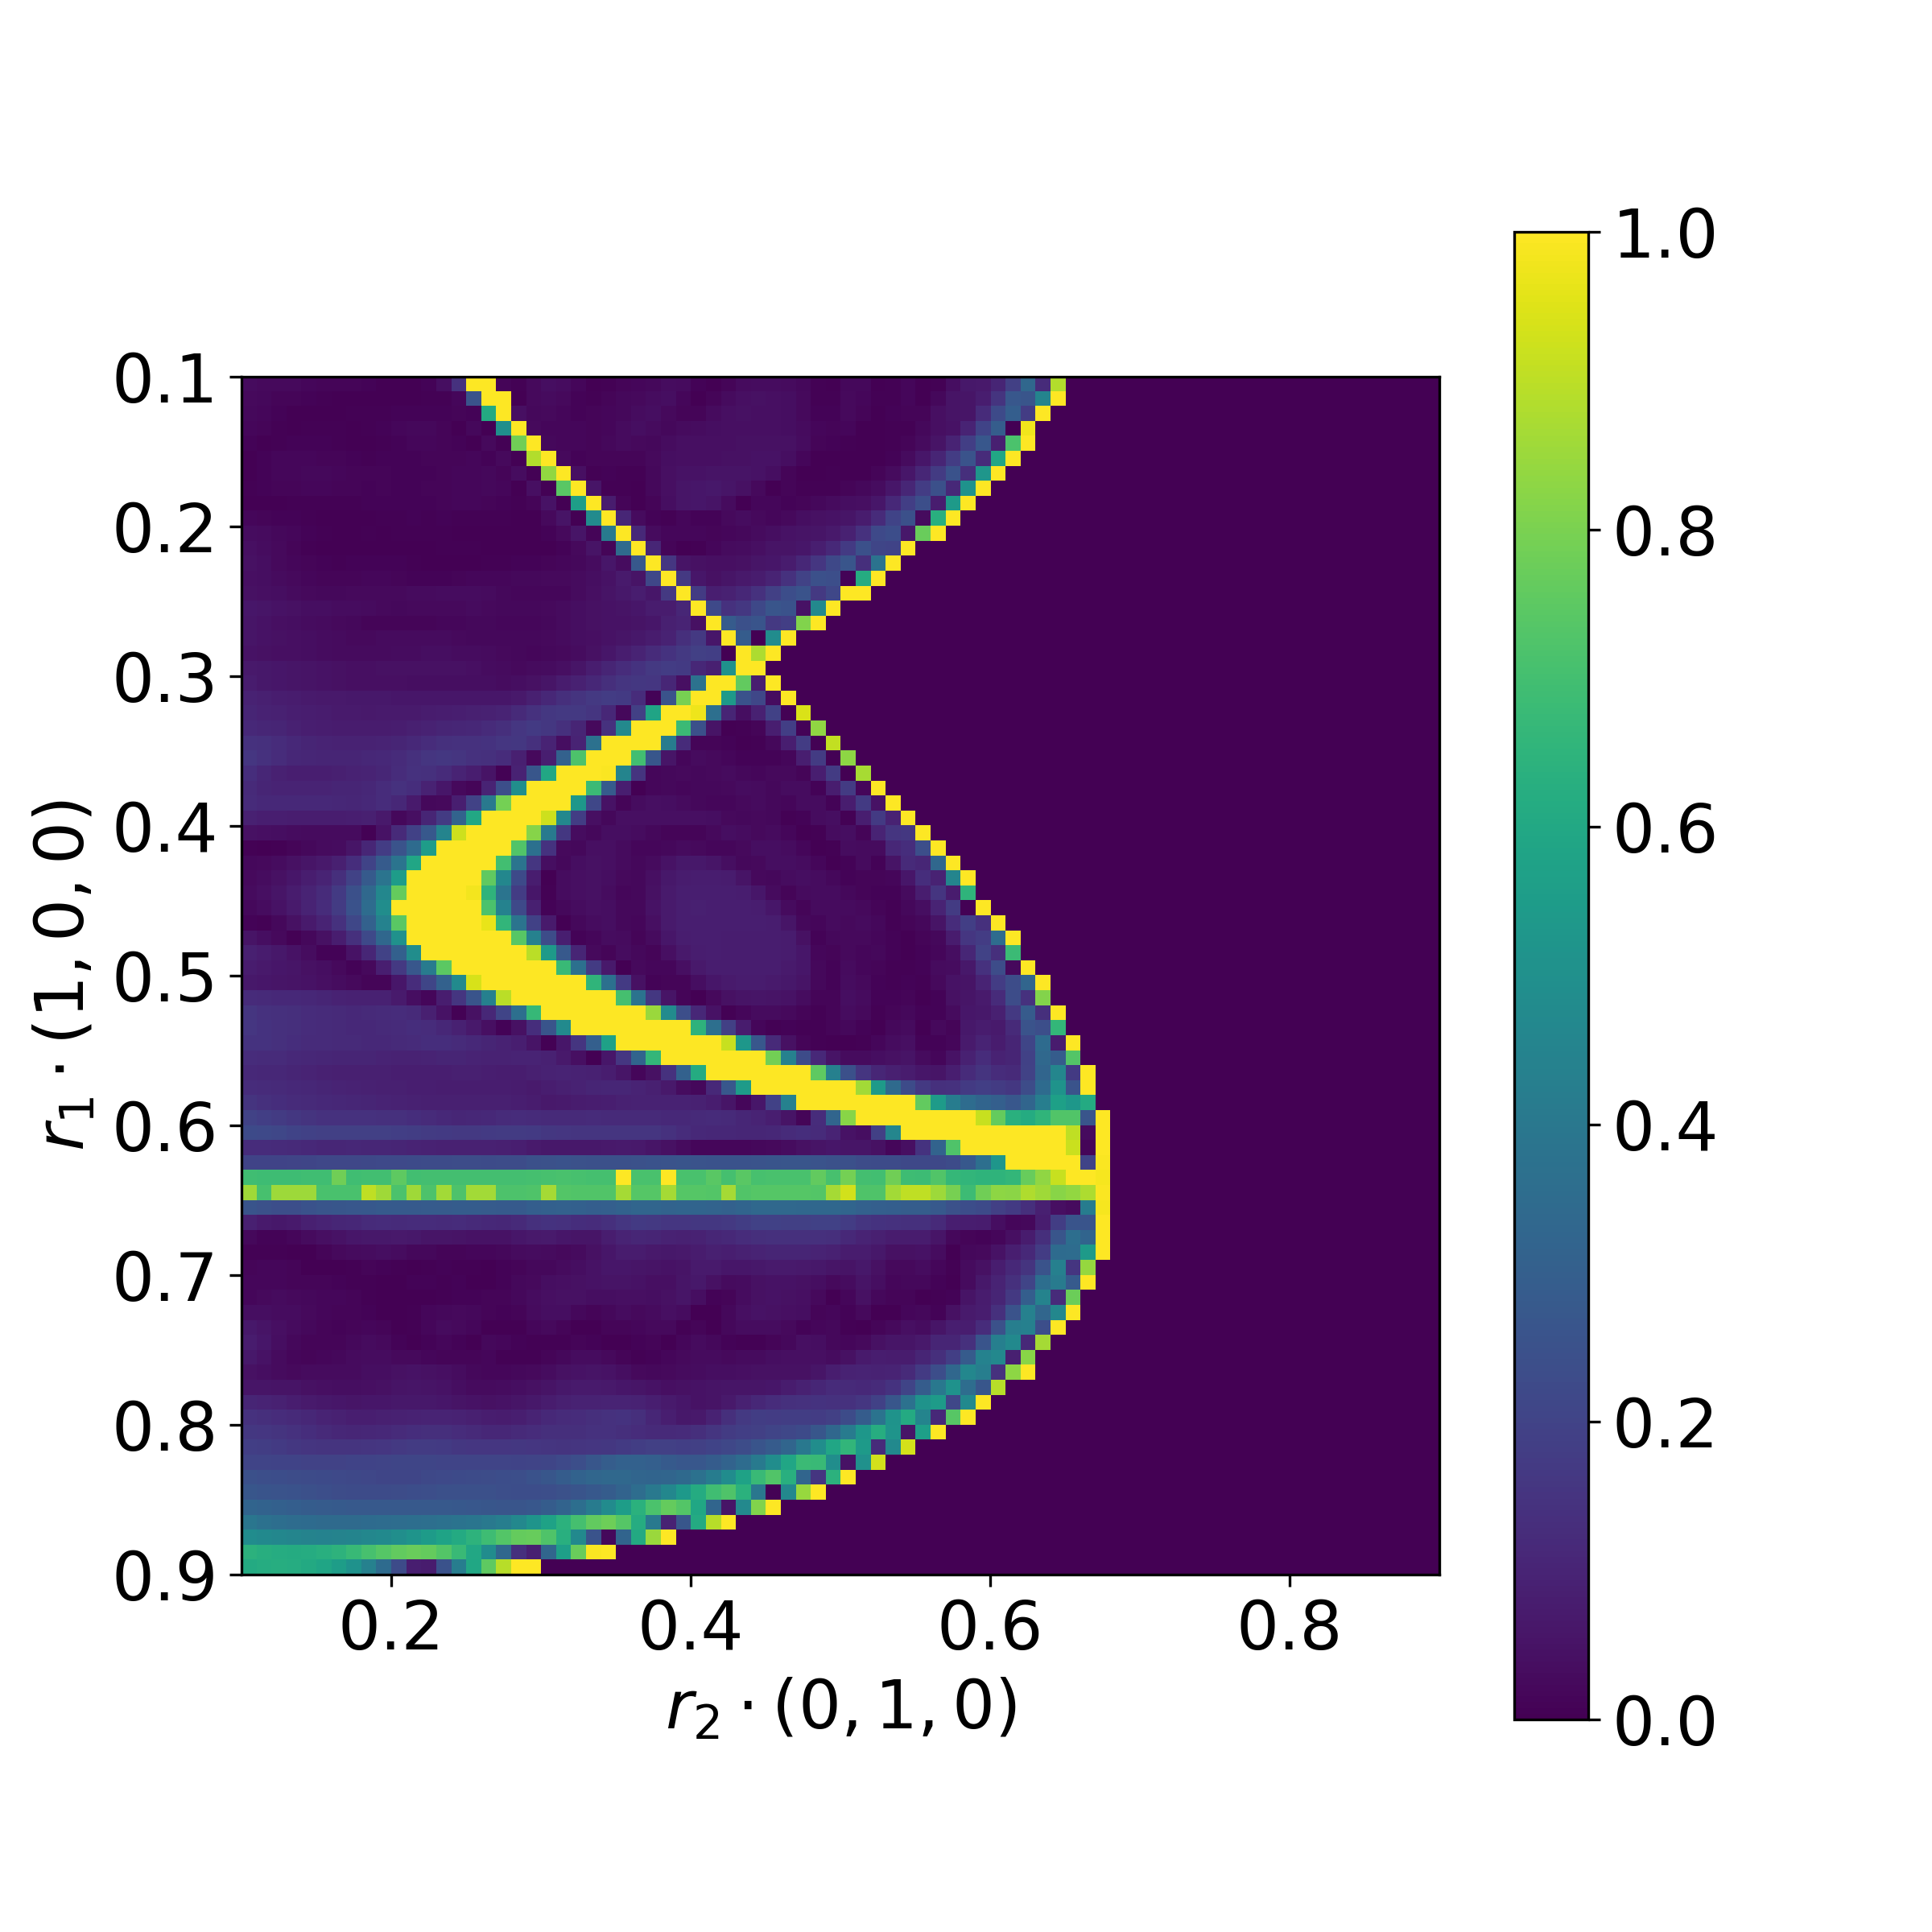
\includegraphics[width=0.4\linewidth]{images/dumbbell-sss-err.png}
    \label{fig:sss-dumbbell-error}}
  \vskip\baselineskip
  \subfigure[$F_{sss}$: precise. The correlation function is undefined (has type
    II discontinuity) at curves A, B and C.]{
    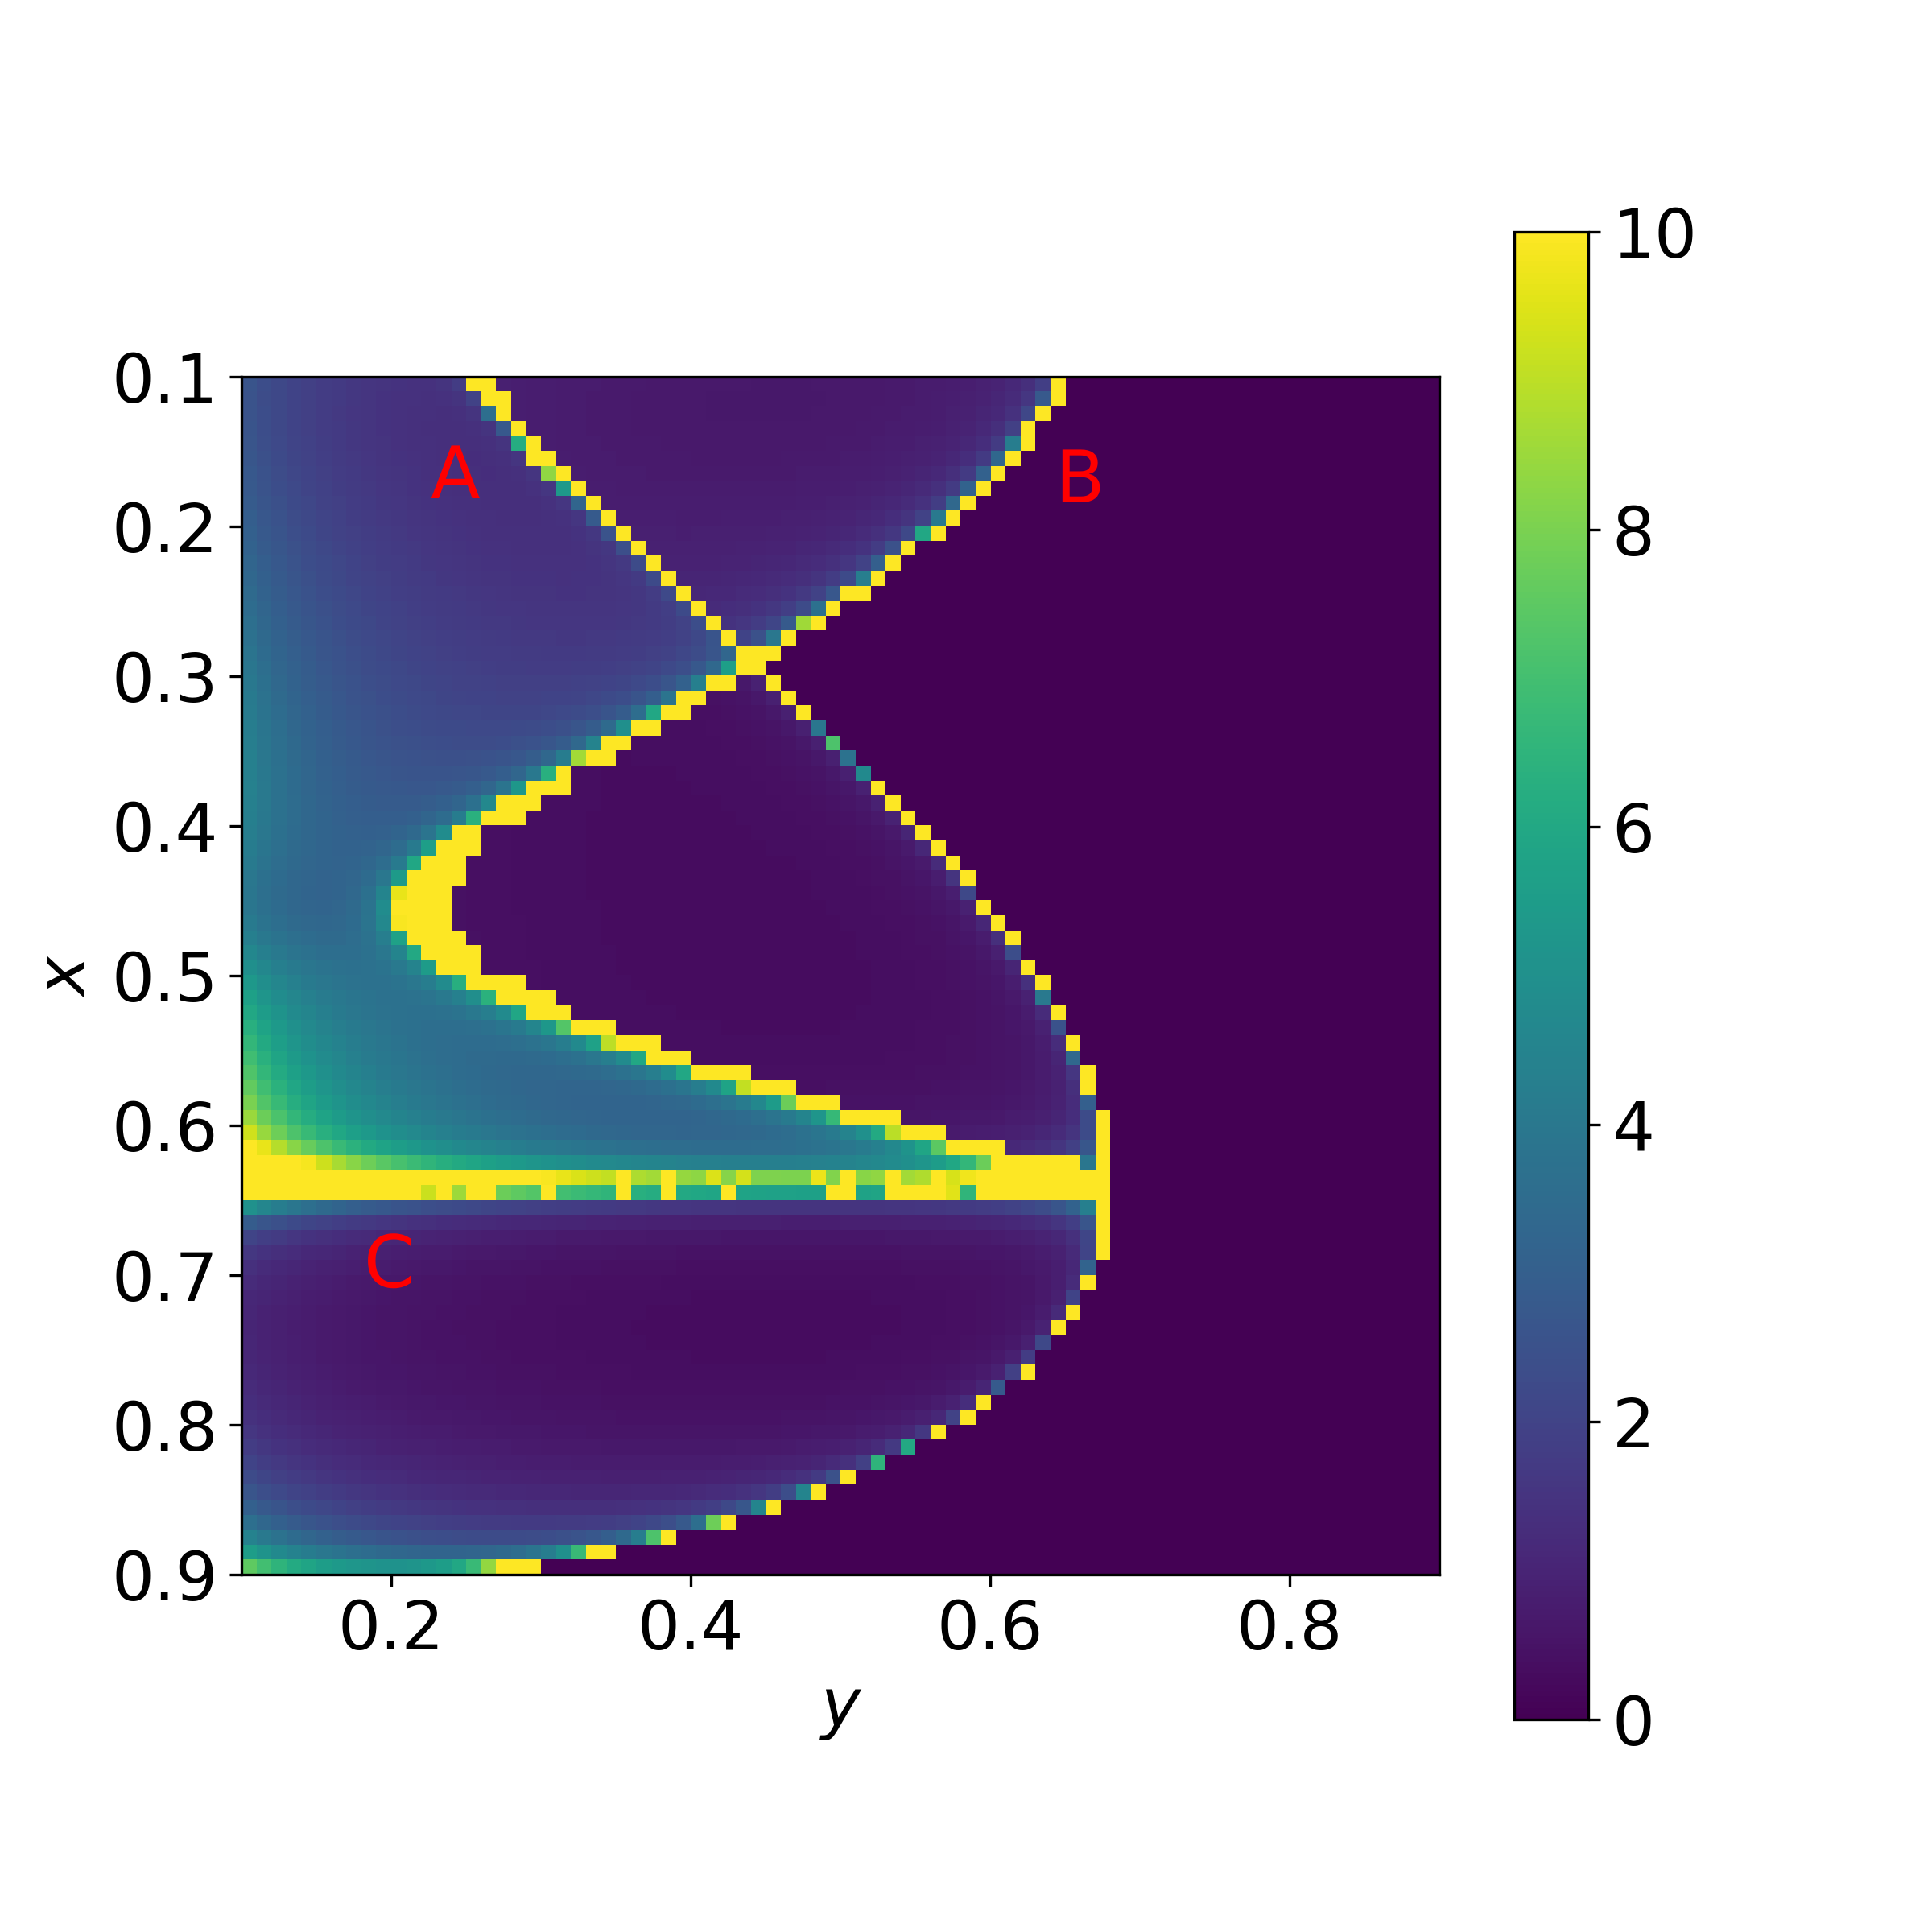
\includegraphics[width=0.4\linewidth]{images/dumbbell-sss-precise.png}
    \label{fig:sss-dumbbell-precise}}
  \hfill
  \subfigure[$F_{sss}$: calculated with our approach]{
    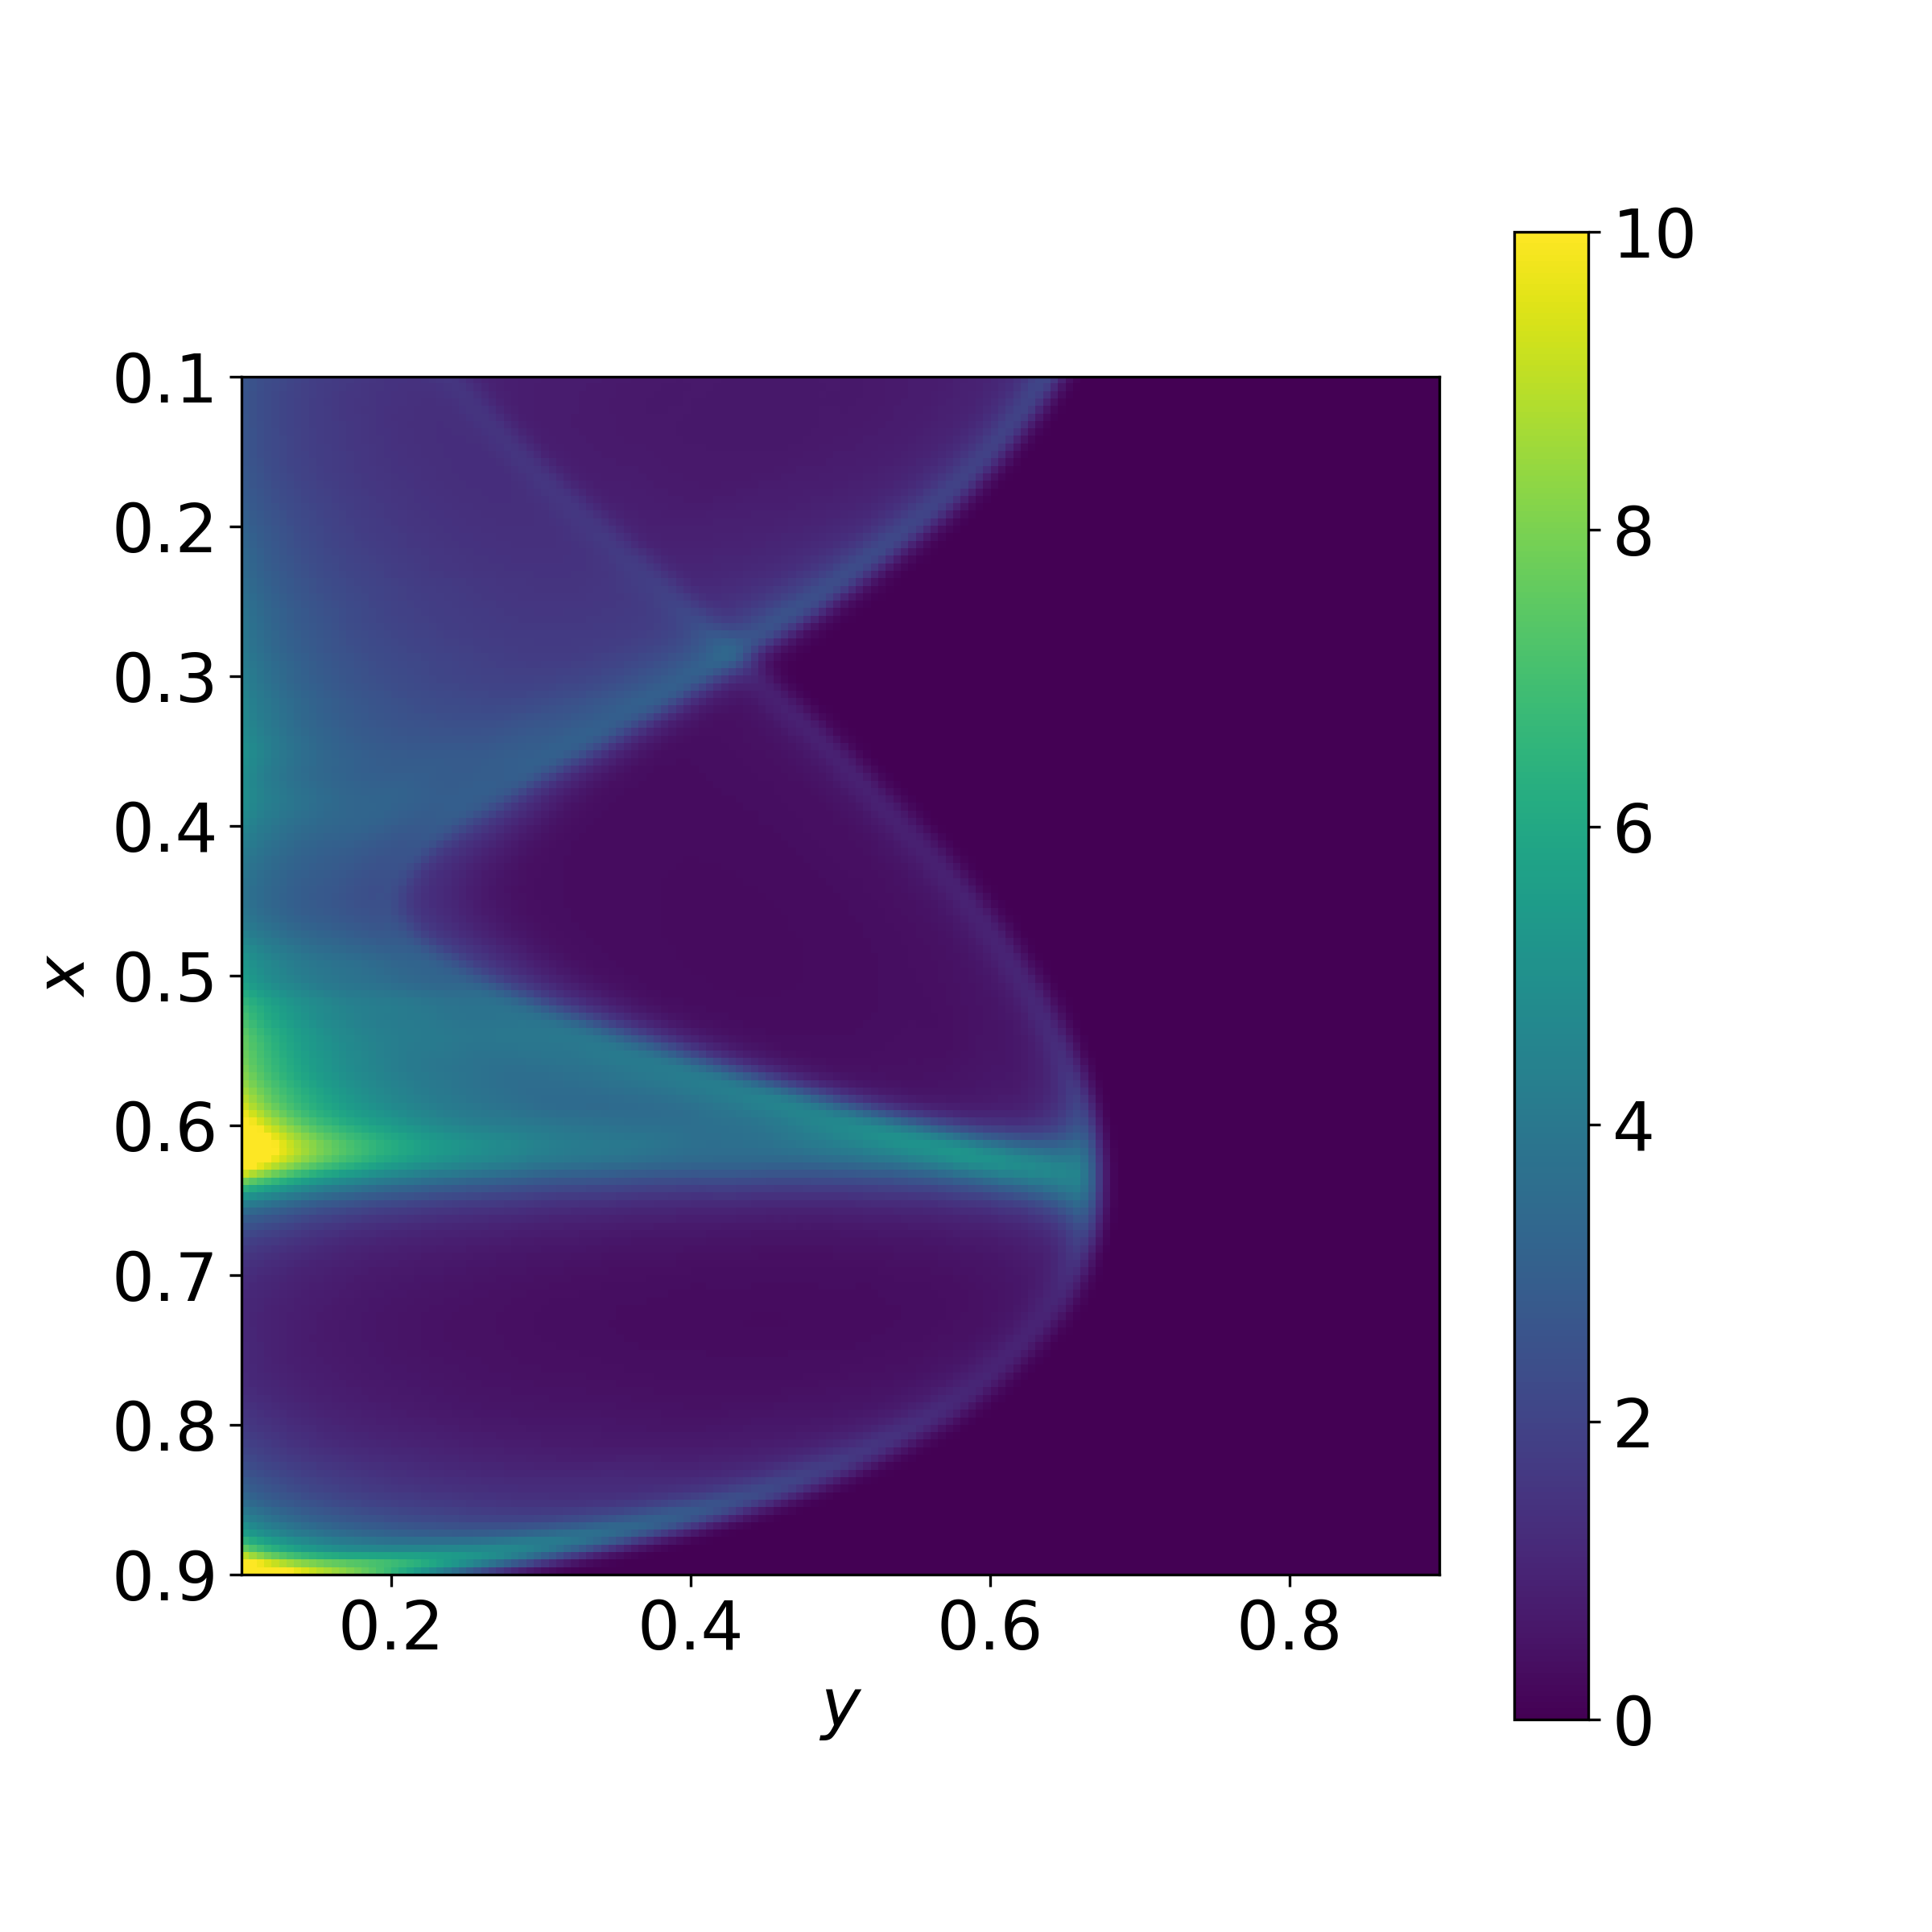
\includegraphics[width=0.4\linewidth]{images/dumbbell-sss-julia.png}}
  \caption[]{A comparison of $F_{sss}$ function calculated using our approach
    with its precise values.}
  \label{fig:sss-verification}
\end{figure*}

To test $F_{ssv}$ and $F_{svv}$ we use the following relations for such a set
$A$ where all non-void phase is covered by a ball with radius $R$:
\begin{align}
  F^n_{ssv}(x_1, x_2) &= F^n_{ss}(x_1) \qquad x_2 > R \\
  F^n_{svv}(x_1, x_2) &= F^n_{sv}(x_1) \qquad x_2 > R
\end{align}
$F_{ss}$ and $F_{sv}$ functions are well-known for a ball of radius $R$ (solid
phase) placed in the center of cube of volume $V$ (void phase):
\begin{align}
  F_{ss}(r, R) &= \frac{1}{V} \left\{
    \begin{array}{ll}
      2\pi R^2/r & \quad r < 2R \\
      0 & \quad \text{otherwise}
    \end{array}
    \right.\\
  F_{sv}(r, R) &= \frac{1}{V} \left\{
    \begin{array}{ll}
      \pi Rr + 2\pi R^2 & \quad r < 2R \\
      4\pi R^2 & \quad \text{otherwise}
    \end{array}
    \right.
\end{align}
The comparison of our algorithm against theory is shown on
\cref{fig:surface-verification}. Radius of the ball is chosen to be $R=0.2$.
\begin{figure*}[tp]
  \centering
  \subfigure[$F_{ssv}$]{
    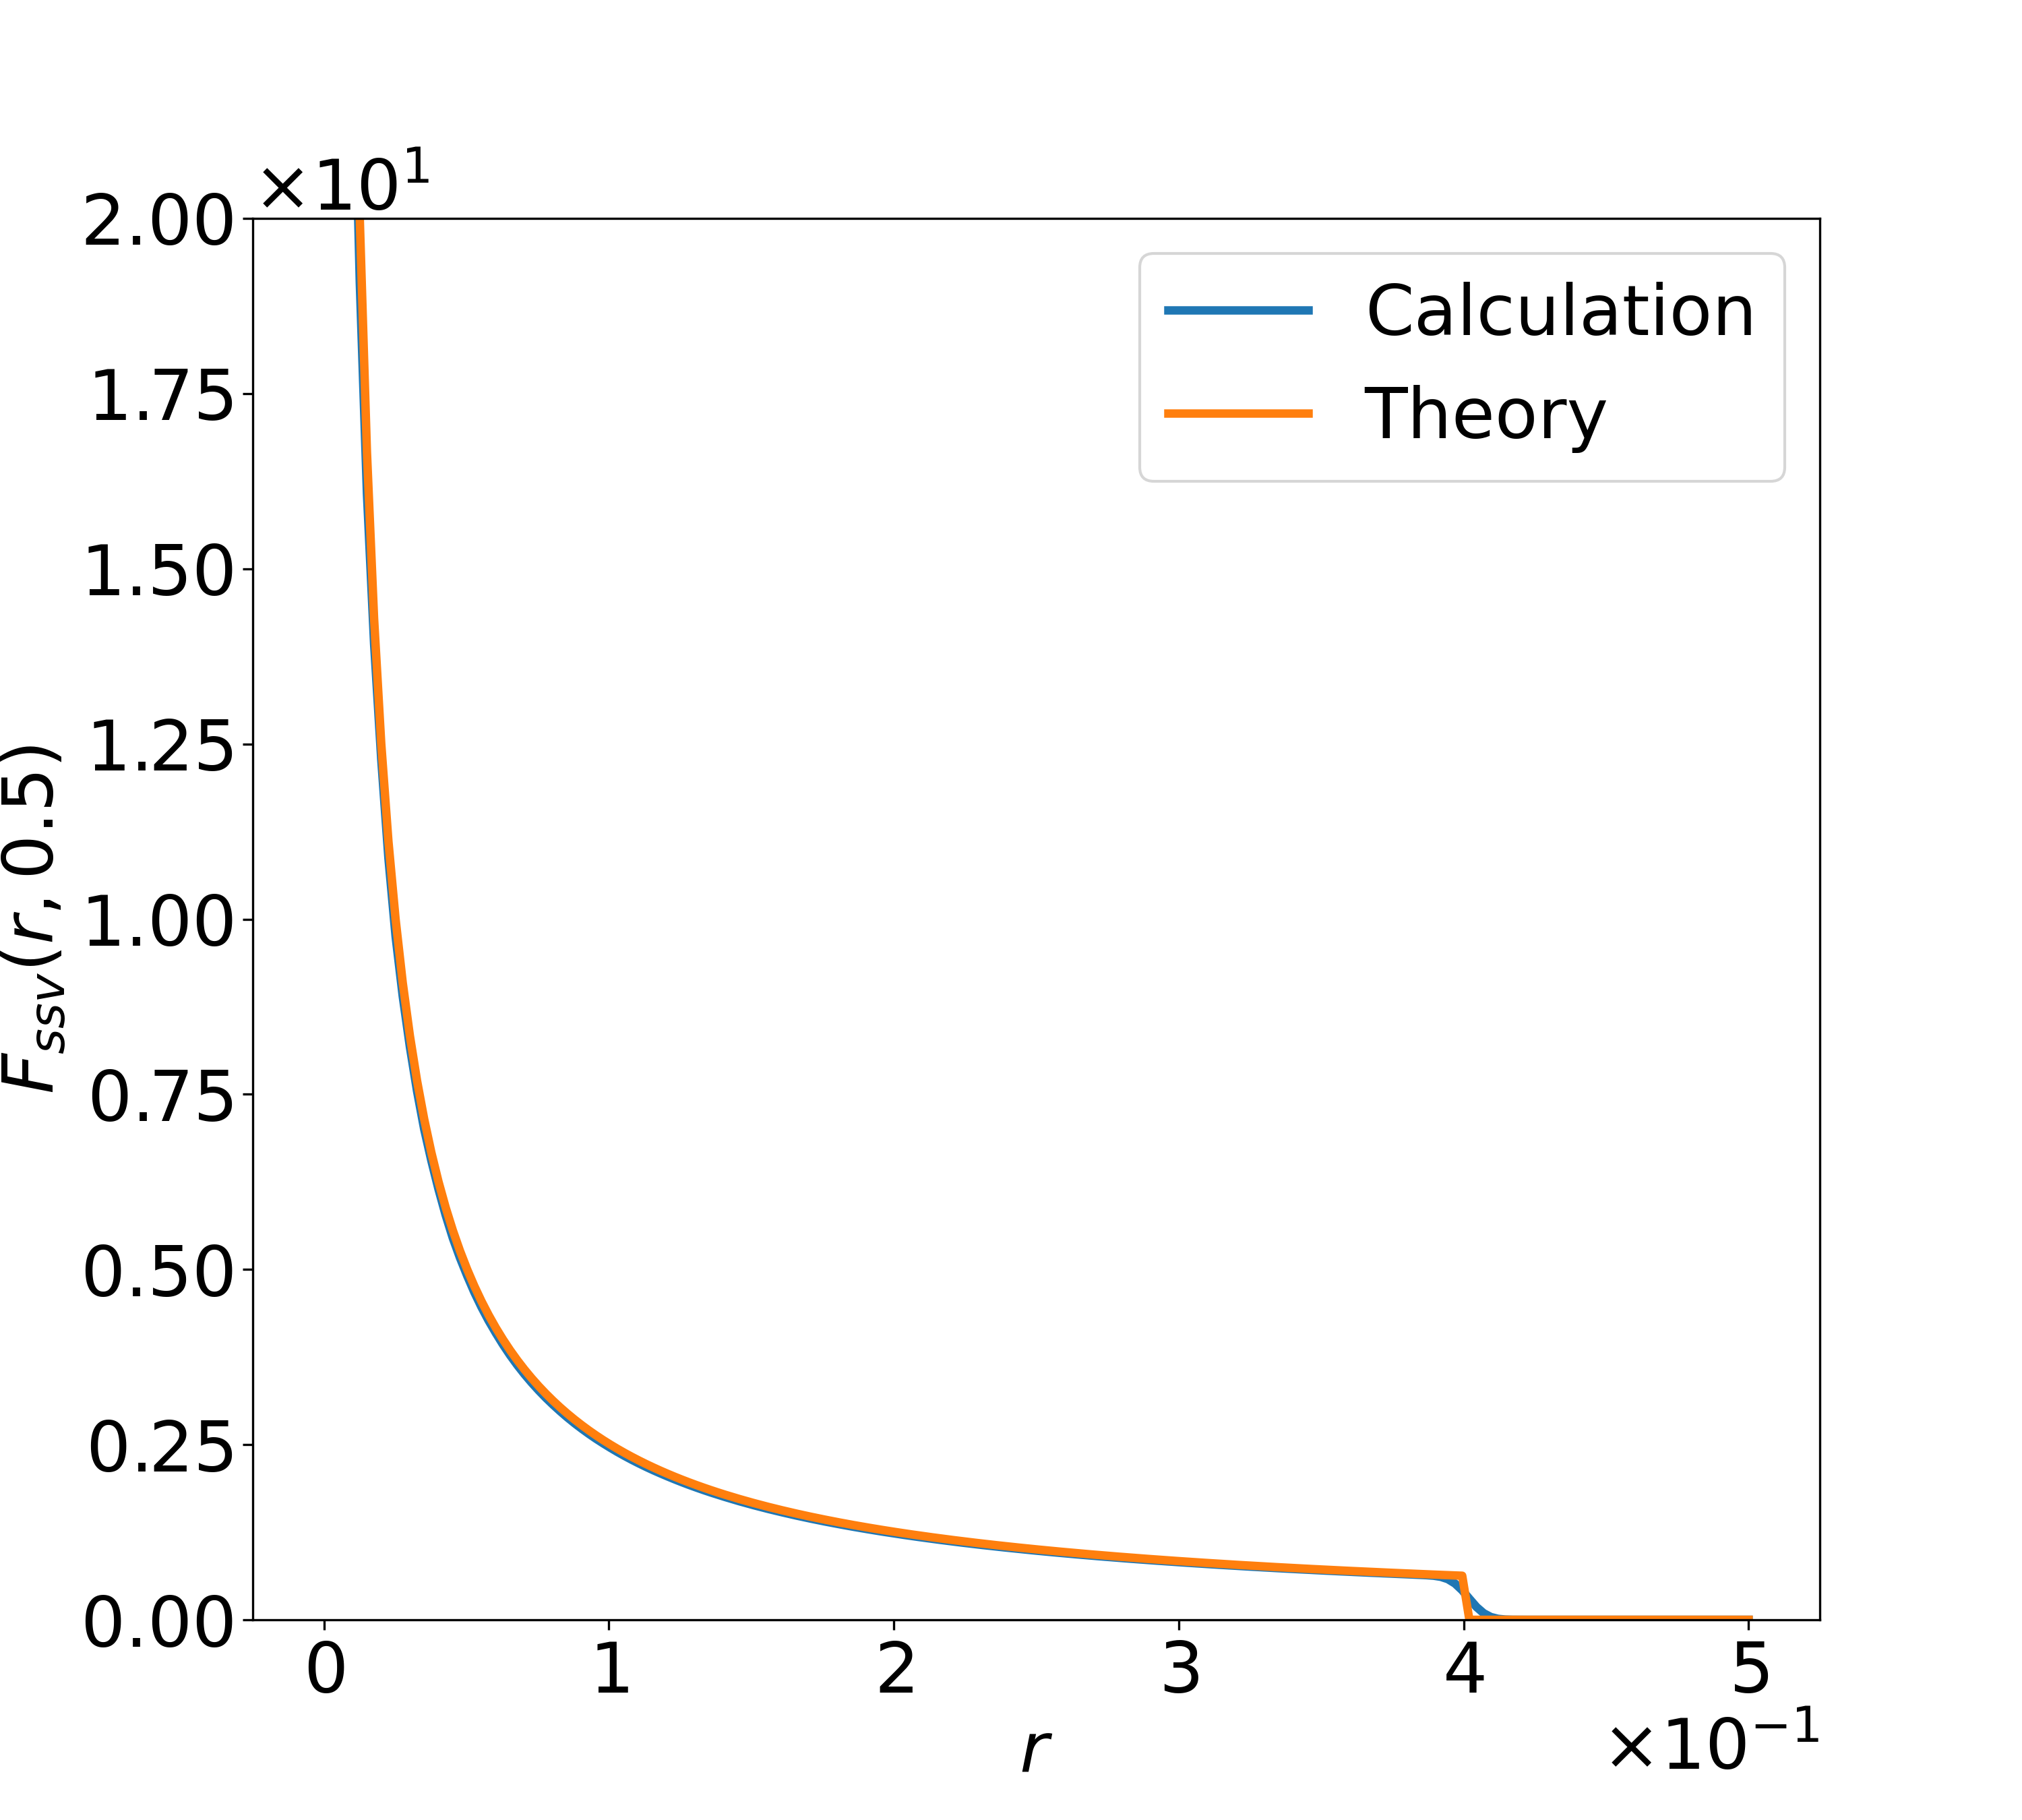
\includegraphics[width=0.4\linewidth]{images/ball-ssv.png}
    \label{fig:balls-ssv}}
  \hfill
  \subfigure[$F_{svv}$]{
    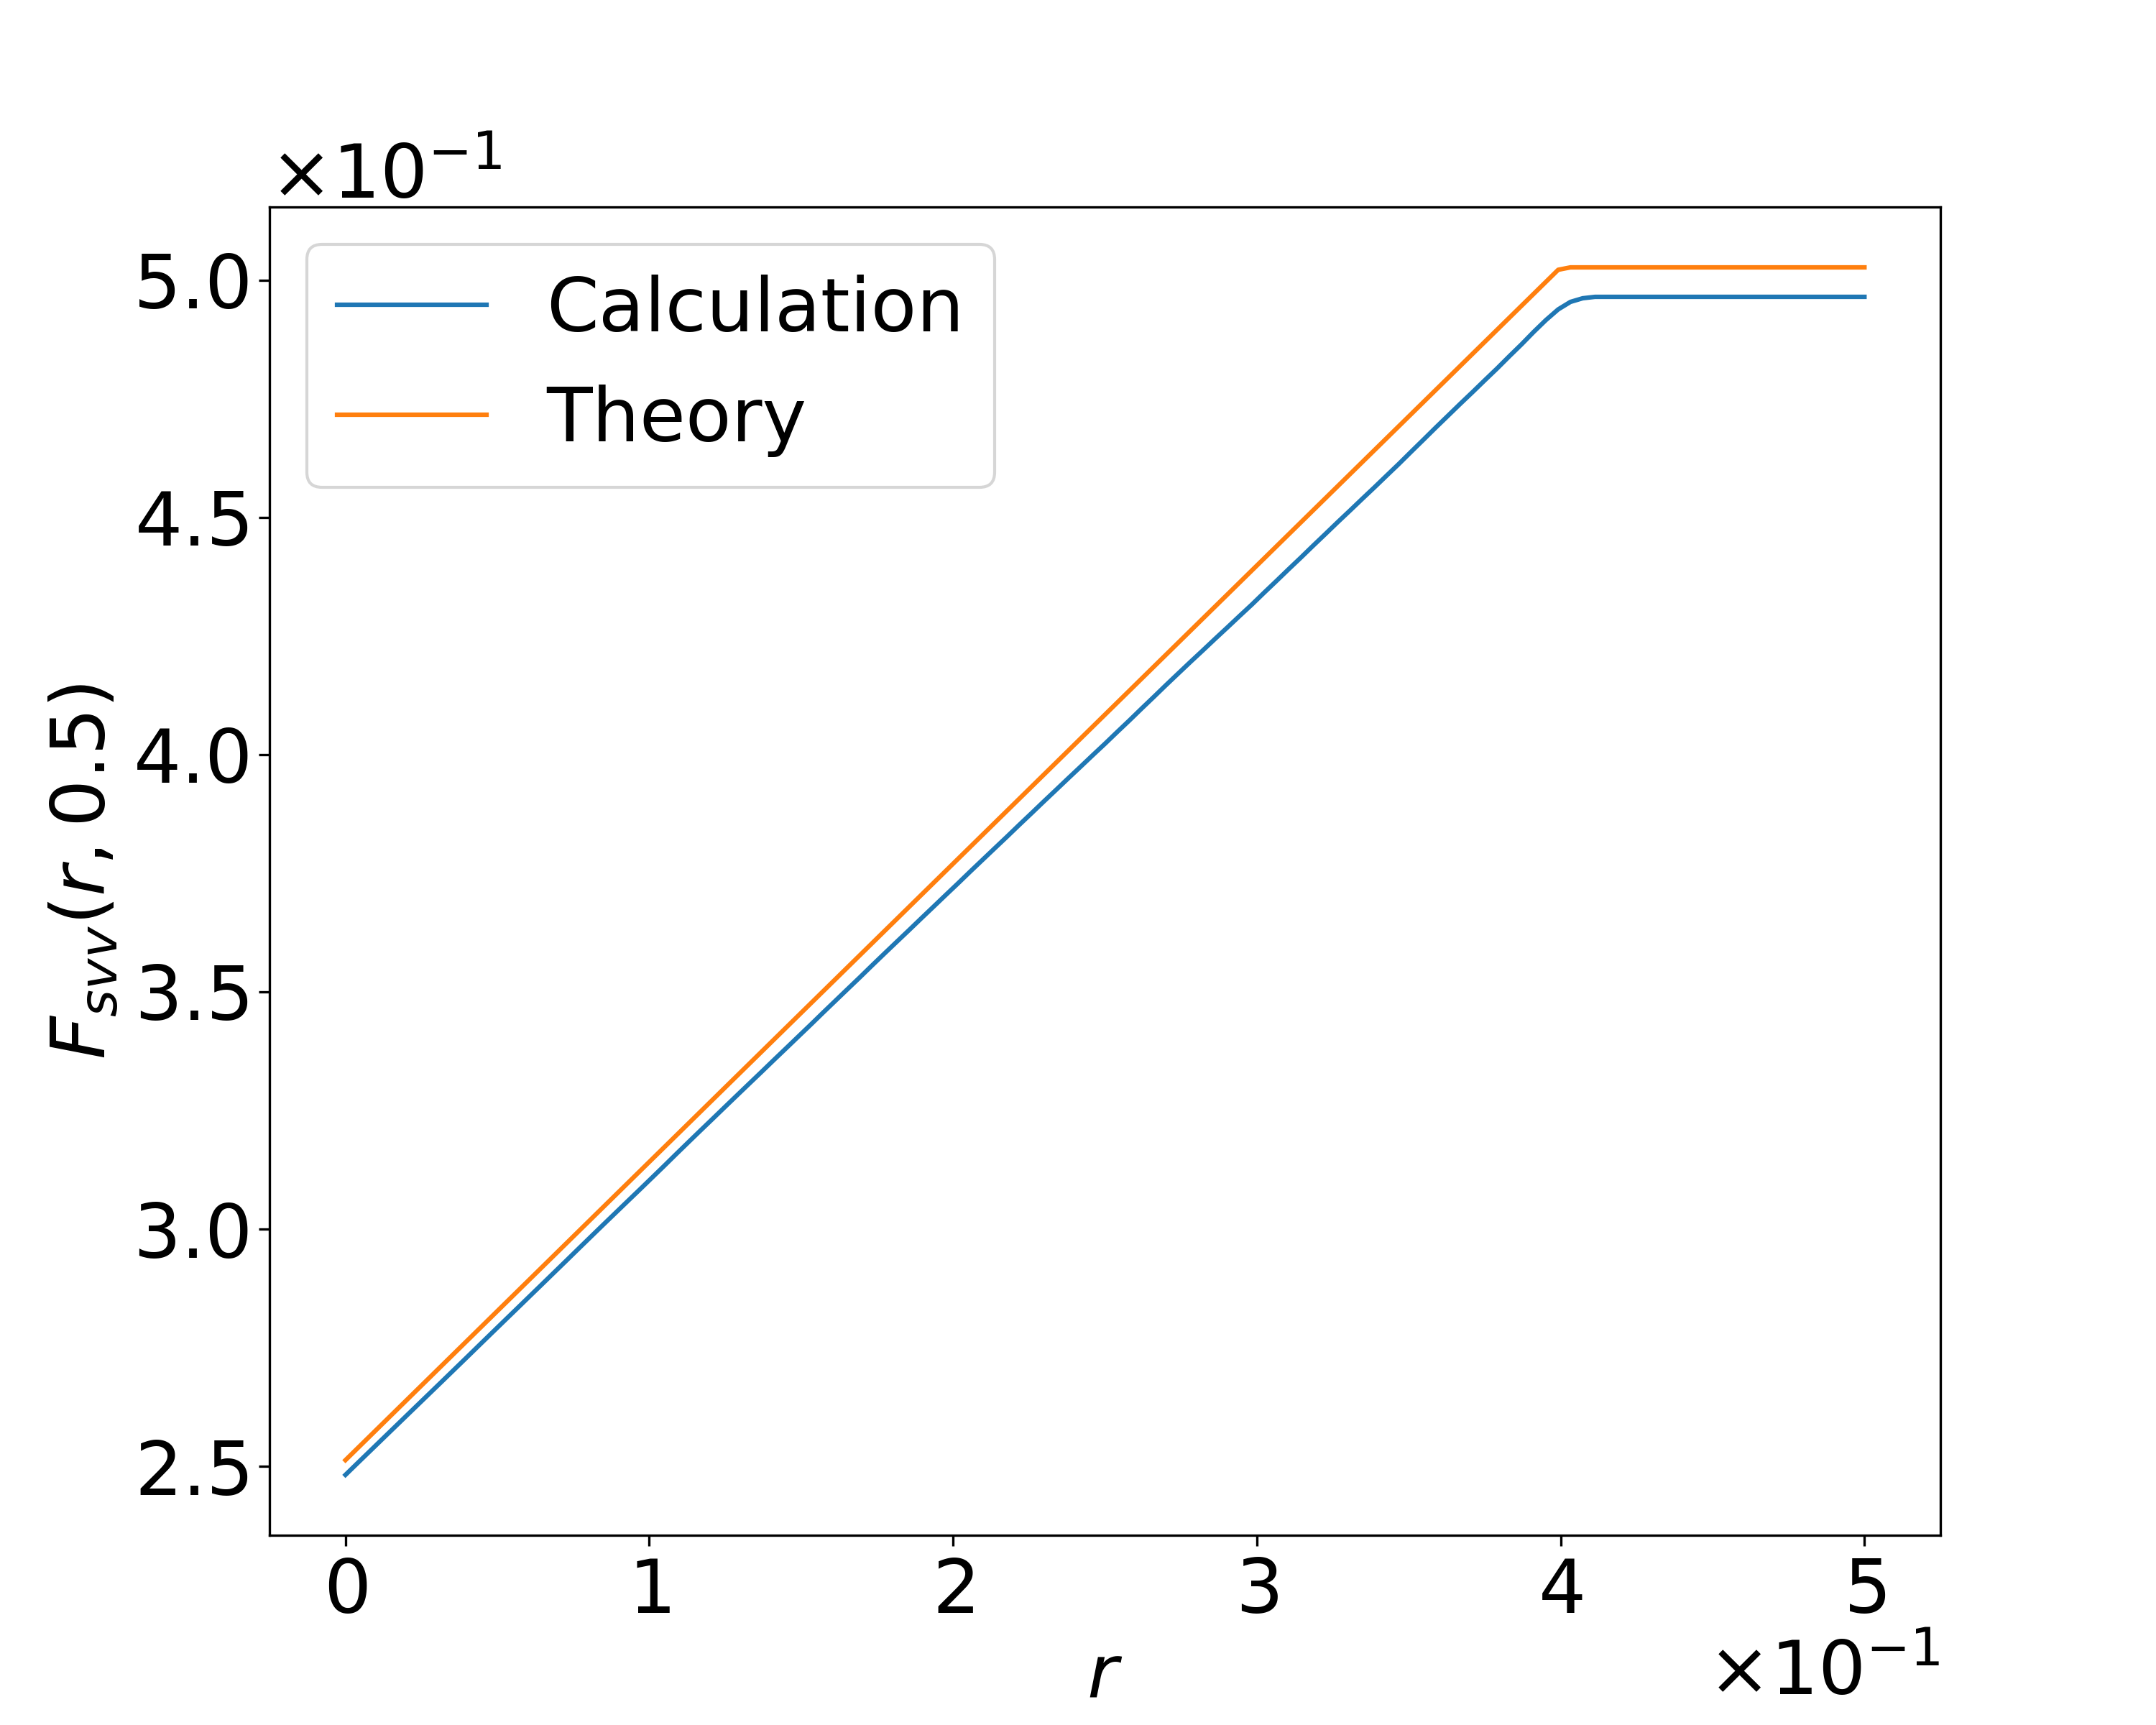
\includegraphics[width=0.4\linewidth]{images/ball-svv.png}
    \label{fig:ball-svv}}
  \caption[]{Comparison of $F_{ssv}$ and $F_{svv}$ functions for a ball with the
    radius $0.2$ with theoretical values.}
  \label{fig:surface-verification}
\end{figure*}

\subsection{Applications to material images}

\begin{table*}[!htp]
  \centering
  \begin{tabular}{|c|c|c|c|c|}
    \hline
    Sample name & Image type & Dimensions (pixels/voxels) & Image resolution ($\mu m$)
    & $C_{0.5}$ \\
    \hline
    Sandstone & XCT &  $500 \times 500 \times 500$ & 2.25 & 0.9703 \\
    Soil & Reconstruction & $500 \times 500 \times 500$ & 0.72 & 0.9431 \\
    Shale & Reconstruction & $160 \times 160 \times 160$ & 2.25 & 0.8912 \\
    Sandstone & SEM &  $1280 \times 869$ & 0.10 & 0.9613 \\
    \hline
  \end{tabular}
  \caption{Summary of samples used for calculation of correlation functions.}
  \label{tab:summary}
\end{table*}
In this section we compute correlation functions for 2- and 3-dimensional porous
media samples. Table \ref{tab:summary} contains information about these
samples. Note that we compute surface correlation functions only for those
samples for which the criterion $C_{0.5} > 0.97$ holds (the two sandstones and
the soil) \cite{samarin2023robust}. Images of the samples are presented on
\cref{fig:samples}. On plots of correlation functions for isotropic samples we
provide a family of curves with the first argument of the correlation function
being fixed. For anisotropic samples we provide heatmaps of correlation
functions where anisotropy can be easily observed.
\begin{figure*}[tp]
  \centering
  \subfigure[Sanstone XCT]{
    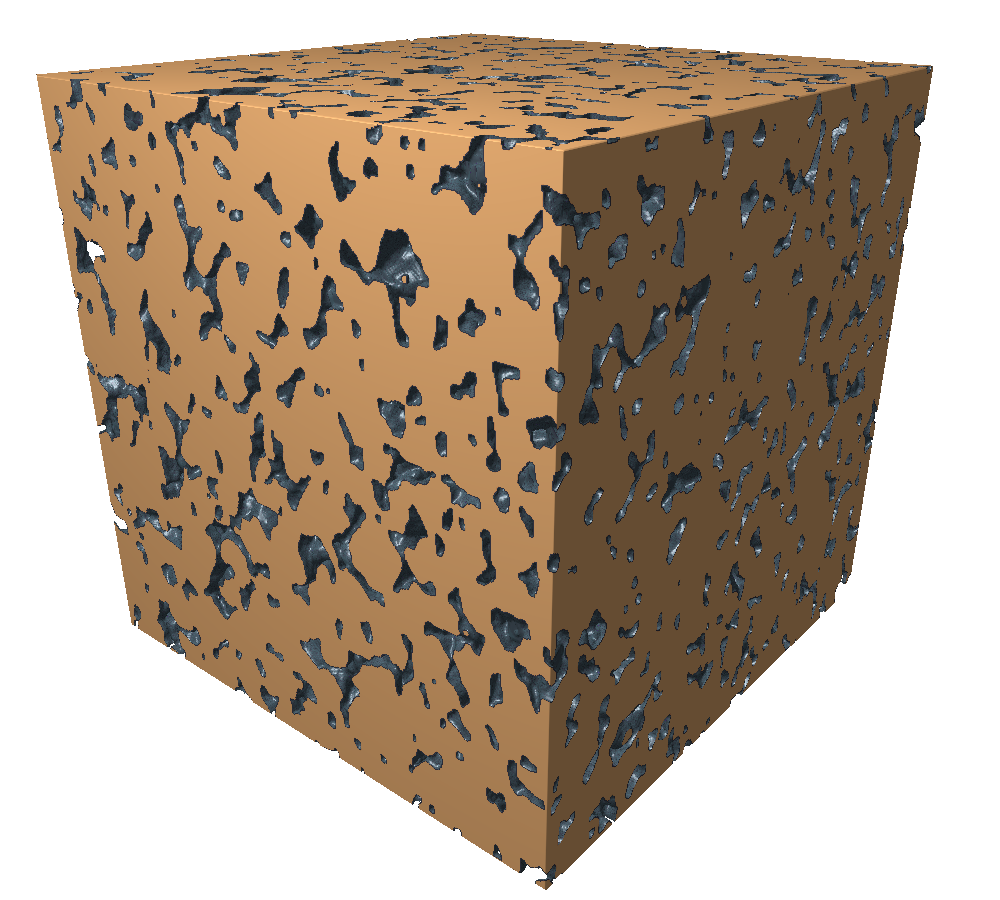
\includegraphics[width=0.4\linewidth]{images/15581.png}
    \label{fig:sample-sandstone-xct}}
  \hfill
  \subfigure[Sandstone SEM (different clusters of void phase are shown in color)]{
    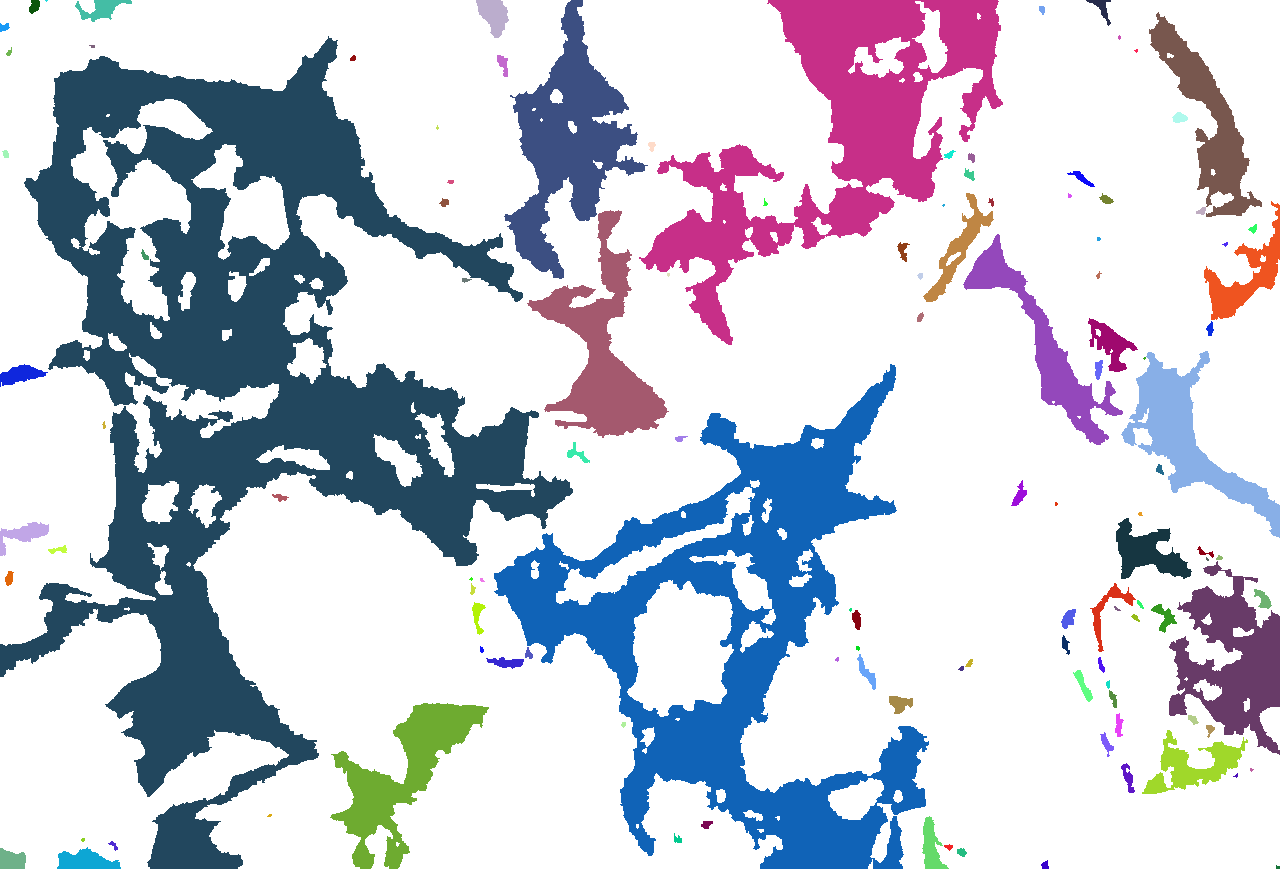
\includegraphics[width=0.4\linewidth, frame]{images/sandstone1.png}
    \label{fig:sample-sandstone}}
  \vskip\baselineskip
  \subfigure[Soil]{
    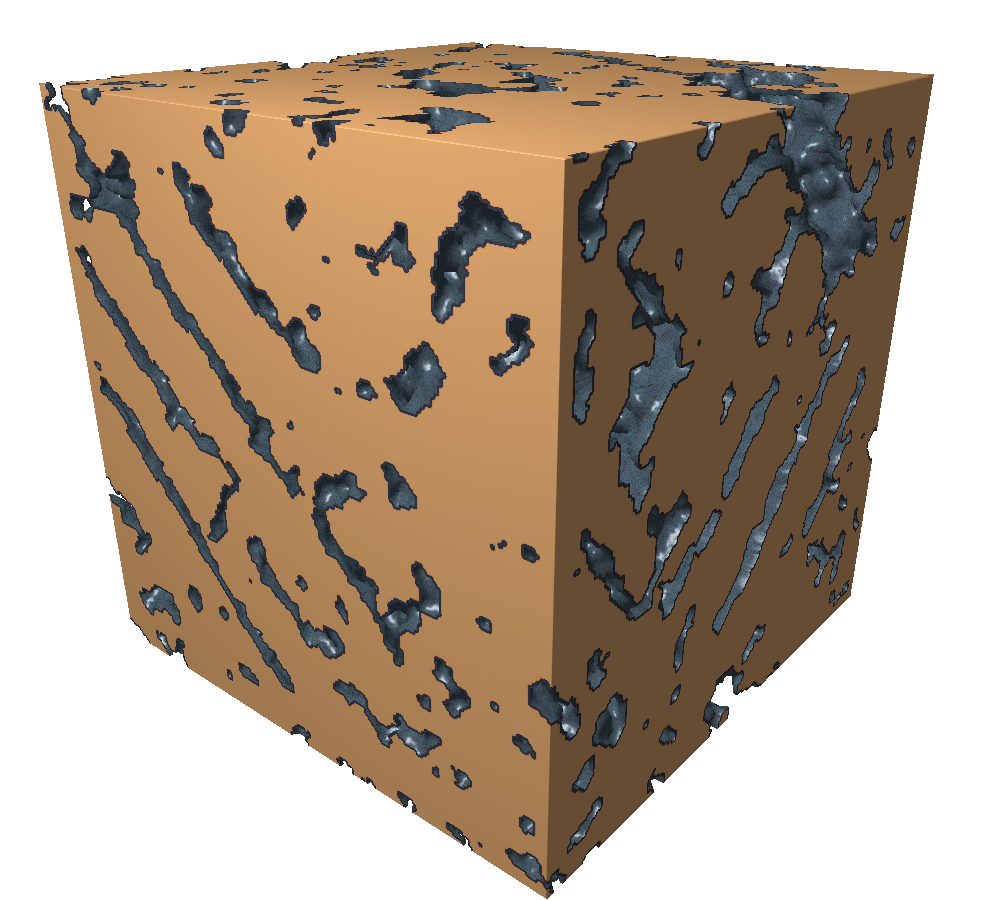
\includegraphics[width=0.4\linewidth]{images/soil.png}
    \label{fig:sample-soil}}
  \hfill
  \subfigure[Shale]{
    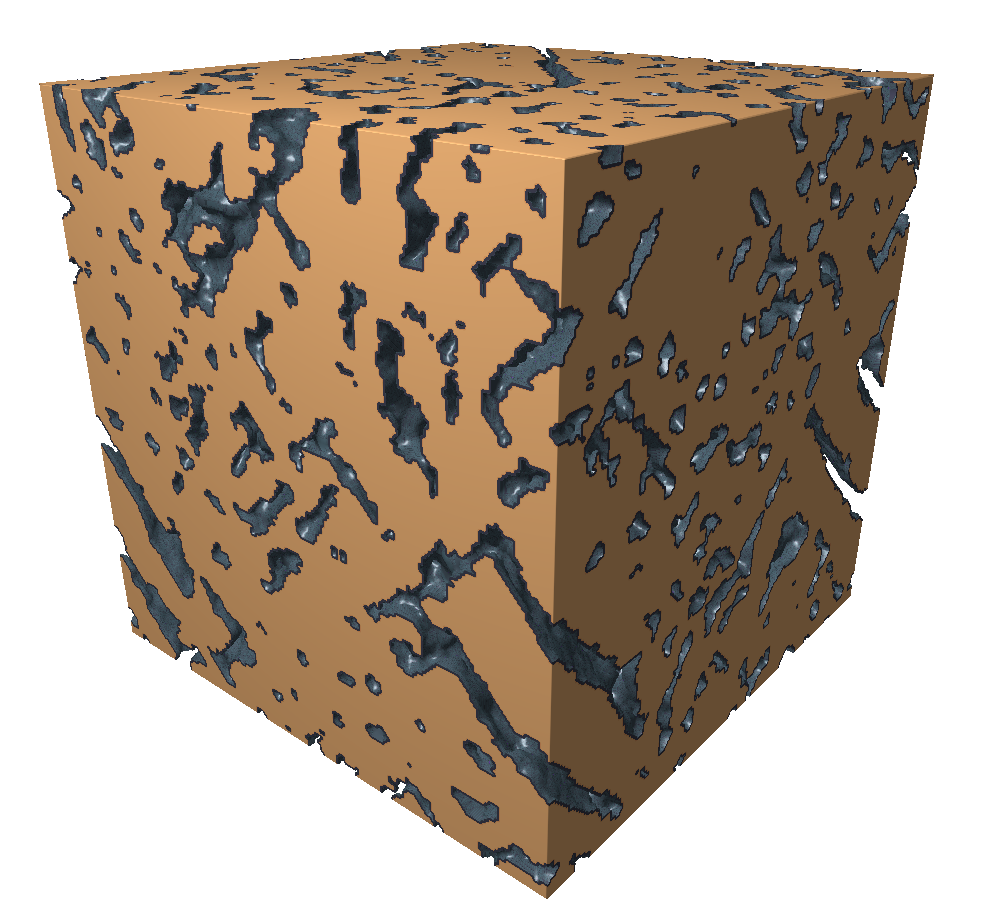
\includegraphics[width=0.4\linewidth]{images/shale.png}
    \label{fig:sample-shale}}
  \caption[]{Images of samples used for calculation of higher-order correlation
    functions.}
  \label{fig:samples}
\end{figure*}

Correlation functions for the XCT sample of a sandstone are on
\cref{fig:sample-sandstone-xct-cf}. The plot of $S_3$ function allows us to
estimate porosity of the sample to be $\sim 0.19$ (note that the curve with
$r_1 = 0$ is actually $S_2$ function). The two-point correlation function
reaches plateau at $r_2 \approx 60 \mu m$ which means that two events
of finding two points in the void phase are independent if the points are
farther than $60 \mu m$ from each other. We see that the sample is isotropic
($S_3(0, 56.25) \approx S_3(56.25, 0)$). From similarity of the $C_3$ and $S_3$
functions it can be stated that the pore phase in this sample forms one big
interconnected pore system.

Correlation functions for the SEM sample (the sandstone) are on
\cref{fig:sample-sandstone-cf}. Porosity of the sample is $\sim 0.3$ as follows
from the plot of $S_3$ function at $r_1 = 0$. The function $S_3(0, r_2)$ reaches
plateau at $r_2 \approx 20\ \mu m$. The sample is highly anisotropic (elongated
along the ordinate). The samples have clusters which are $\sim 45\ \mu m$ in
diameter.

The anisotropic samples (the soil and the shale) were preliminarily rotated with
periodic boundary conditions to align elongated pores with coordinate
axes. Rotated samples are presented on \cref{fig:samples-rot} and heatmaps of
$S_3$ function for these samples -- on \cref{fig:heatmaps}. Based on the
analysis of correlation functions it is evident that elongated clusters of the
void phase within the Soil sample form a structure which resembles a regular
grid with spacing of about $60 \mu m$. The sample of shale shows less regular
yet still anisotropic structure. We provide the rest of correlation functions
for the sample of soil on \cref{fig:soil-maps} - \highlight{and what can we see
  here?}.

\begin{figure*}[tp]
  \centering
  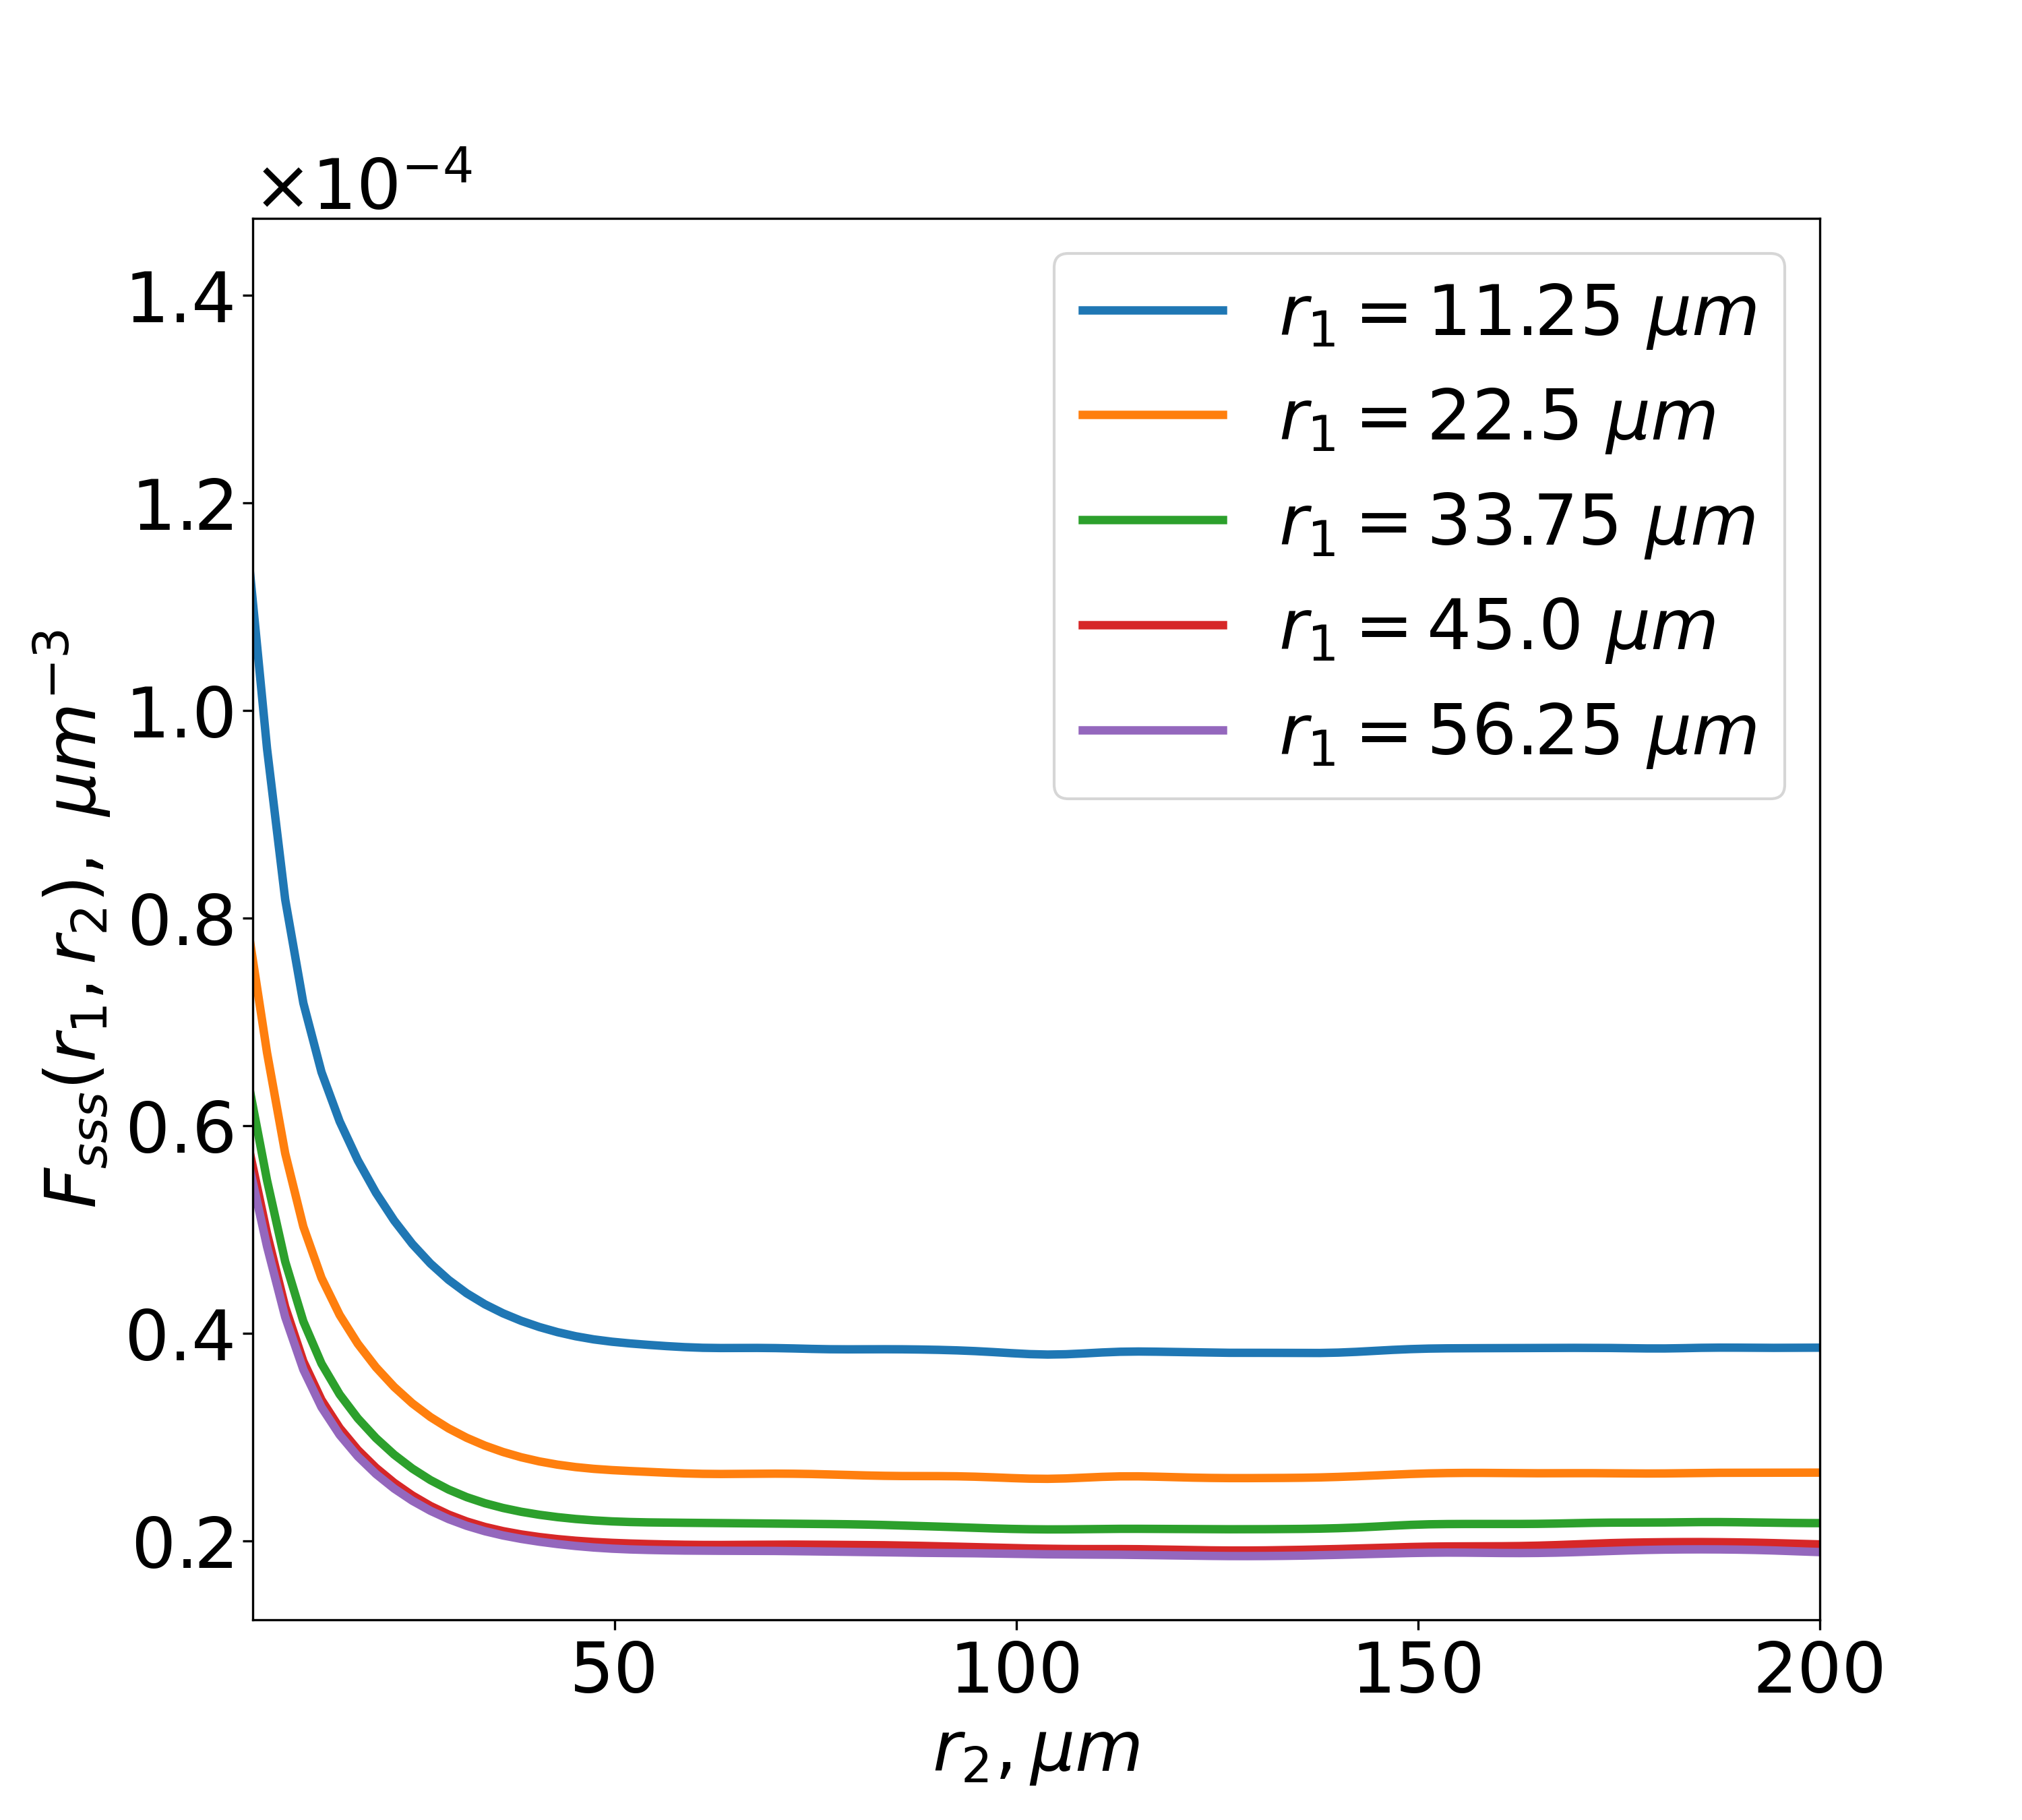
\includegraphics[width=0.4\linewidth]{images/15581-surf3.png}
  \hfill
  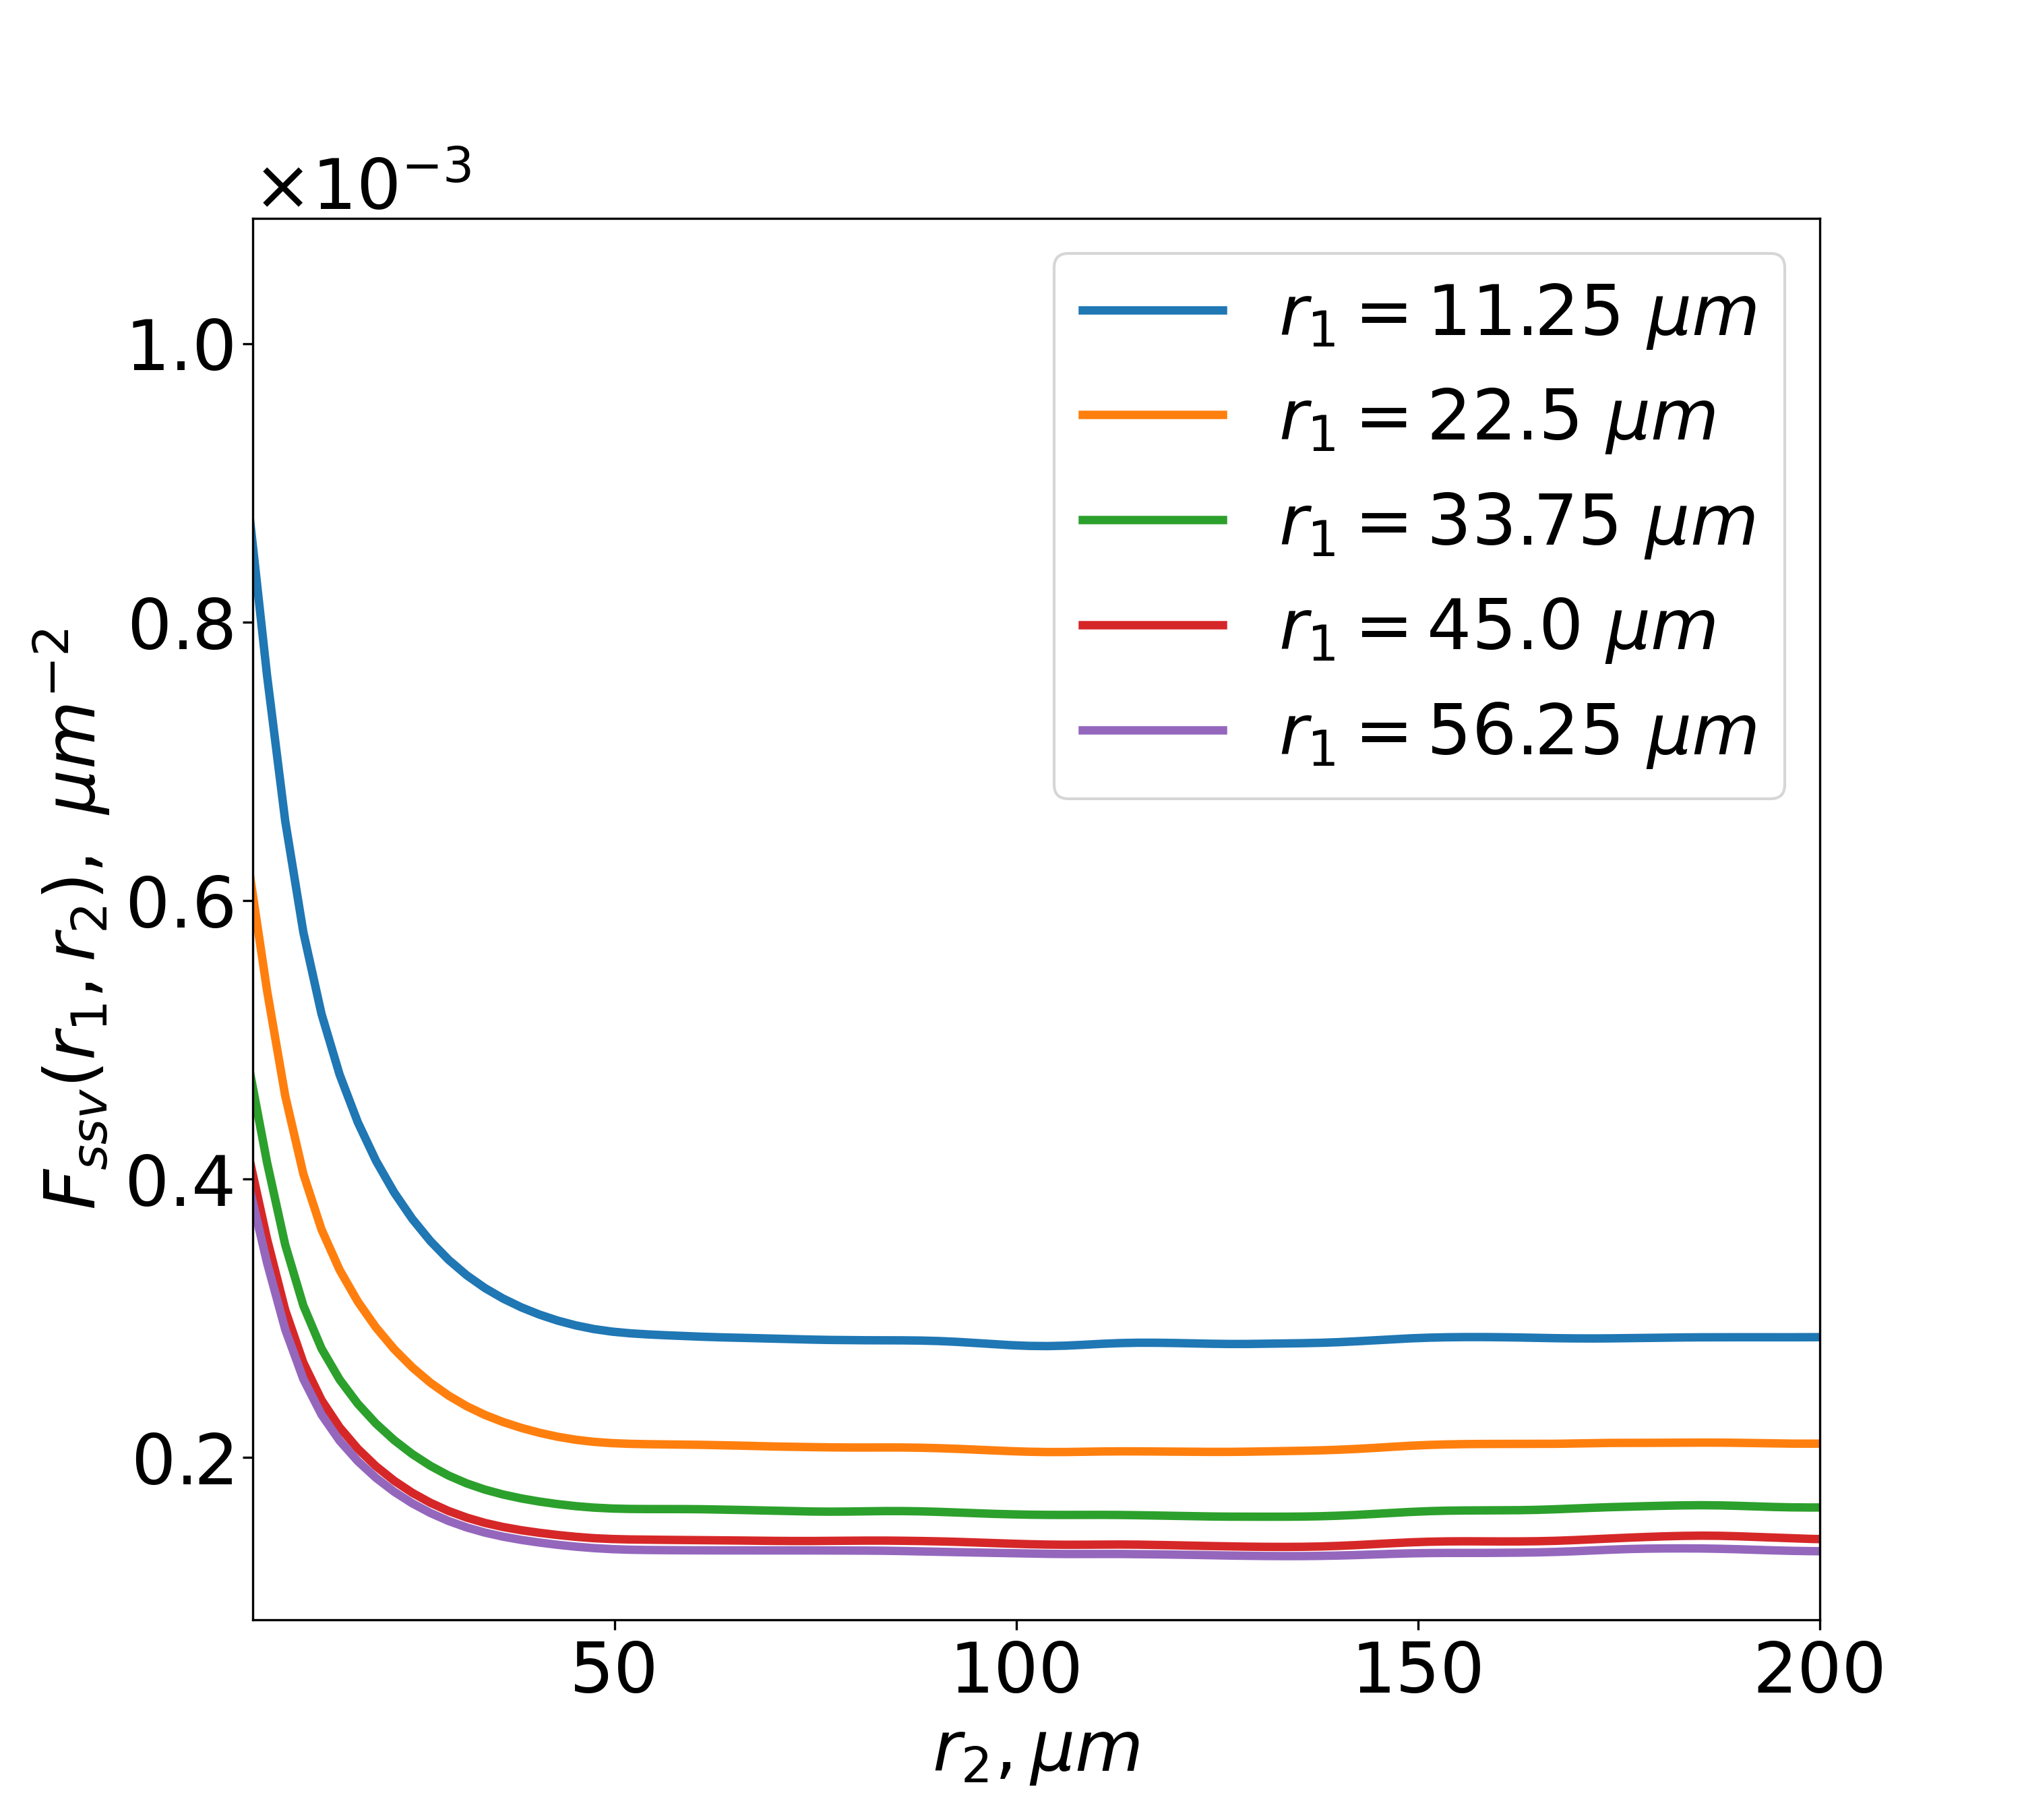
\includegraphics[width=0.4\linewidth]{images/15581-surf2void.png}
  \vskip\baselineskip
  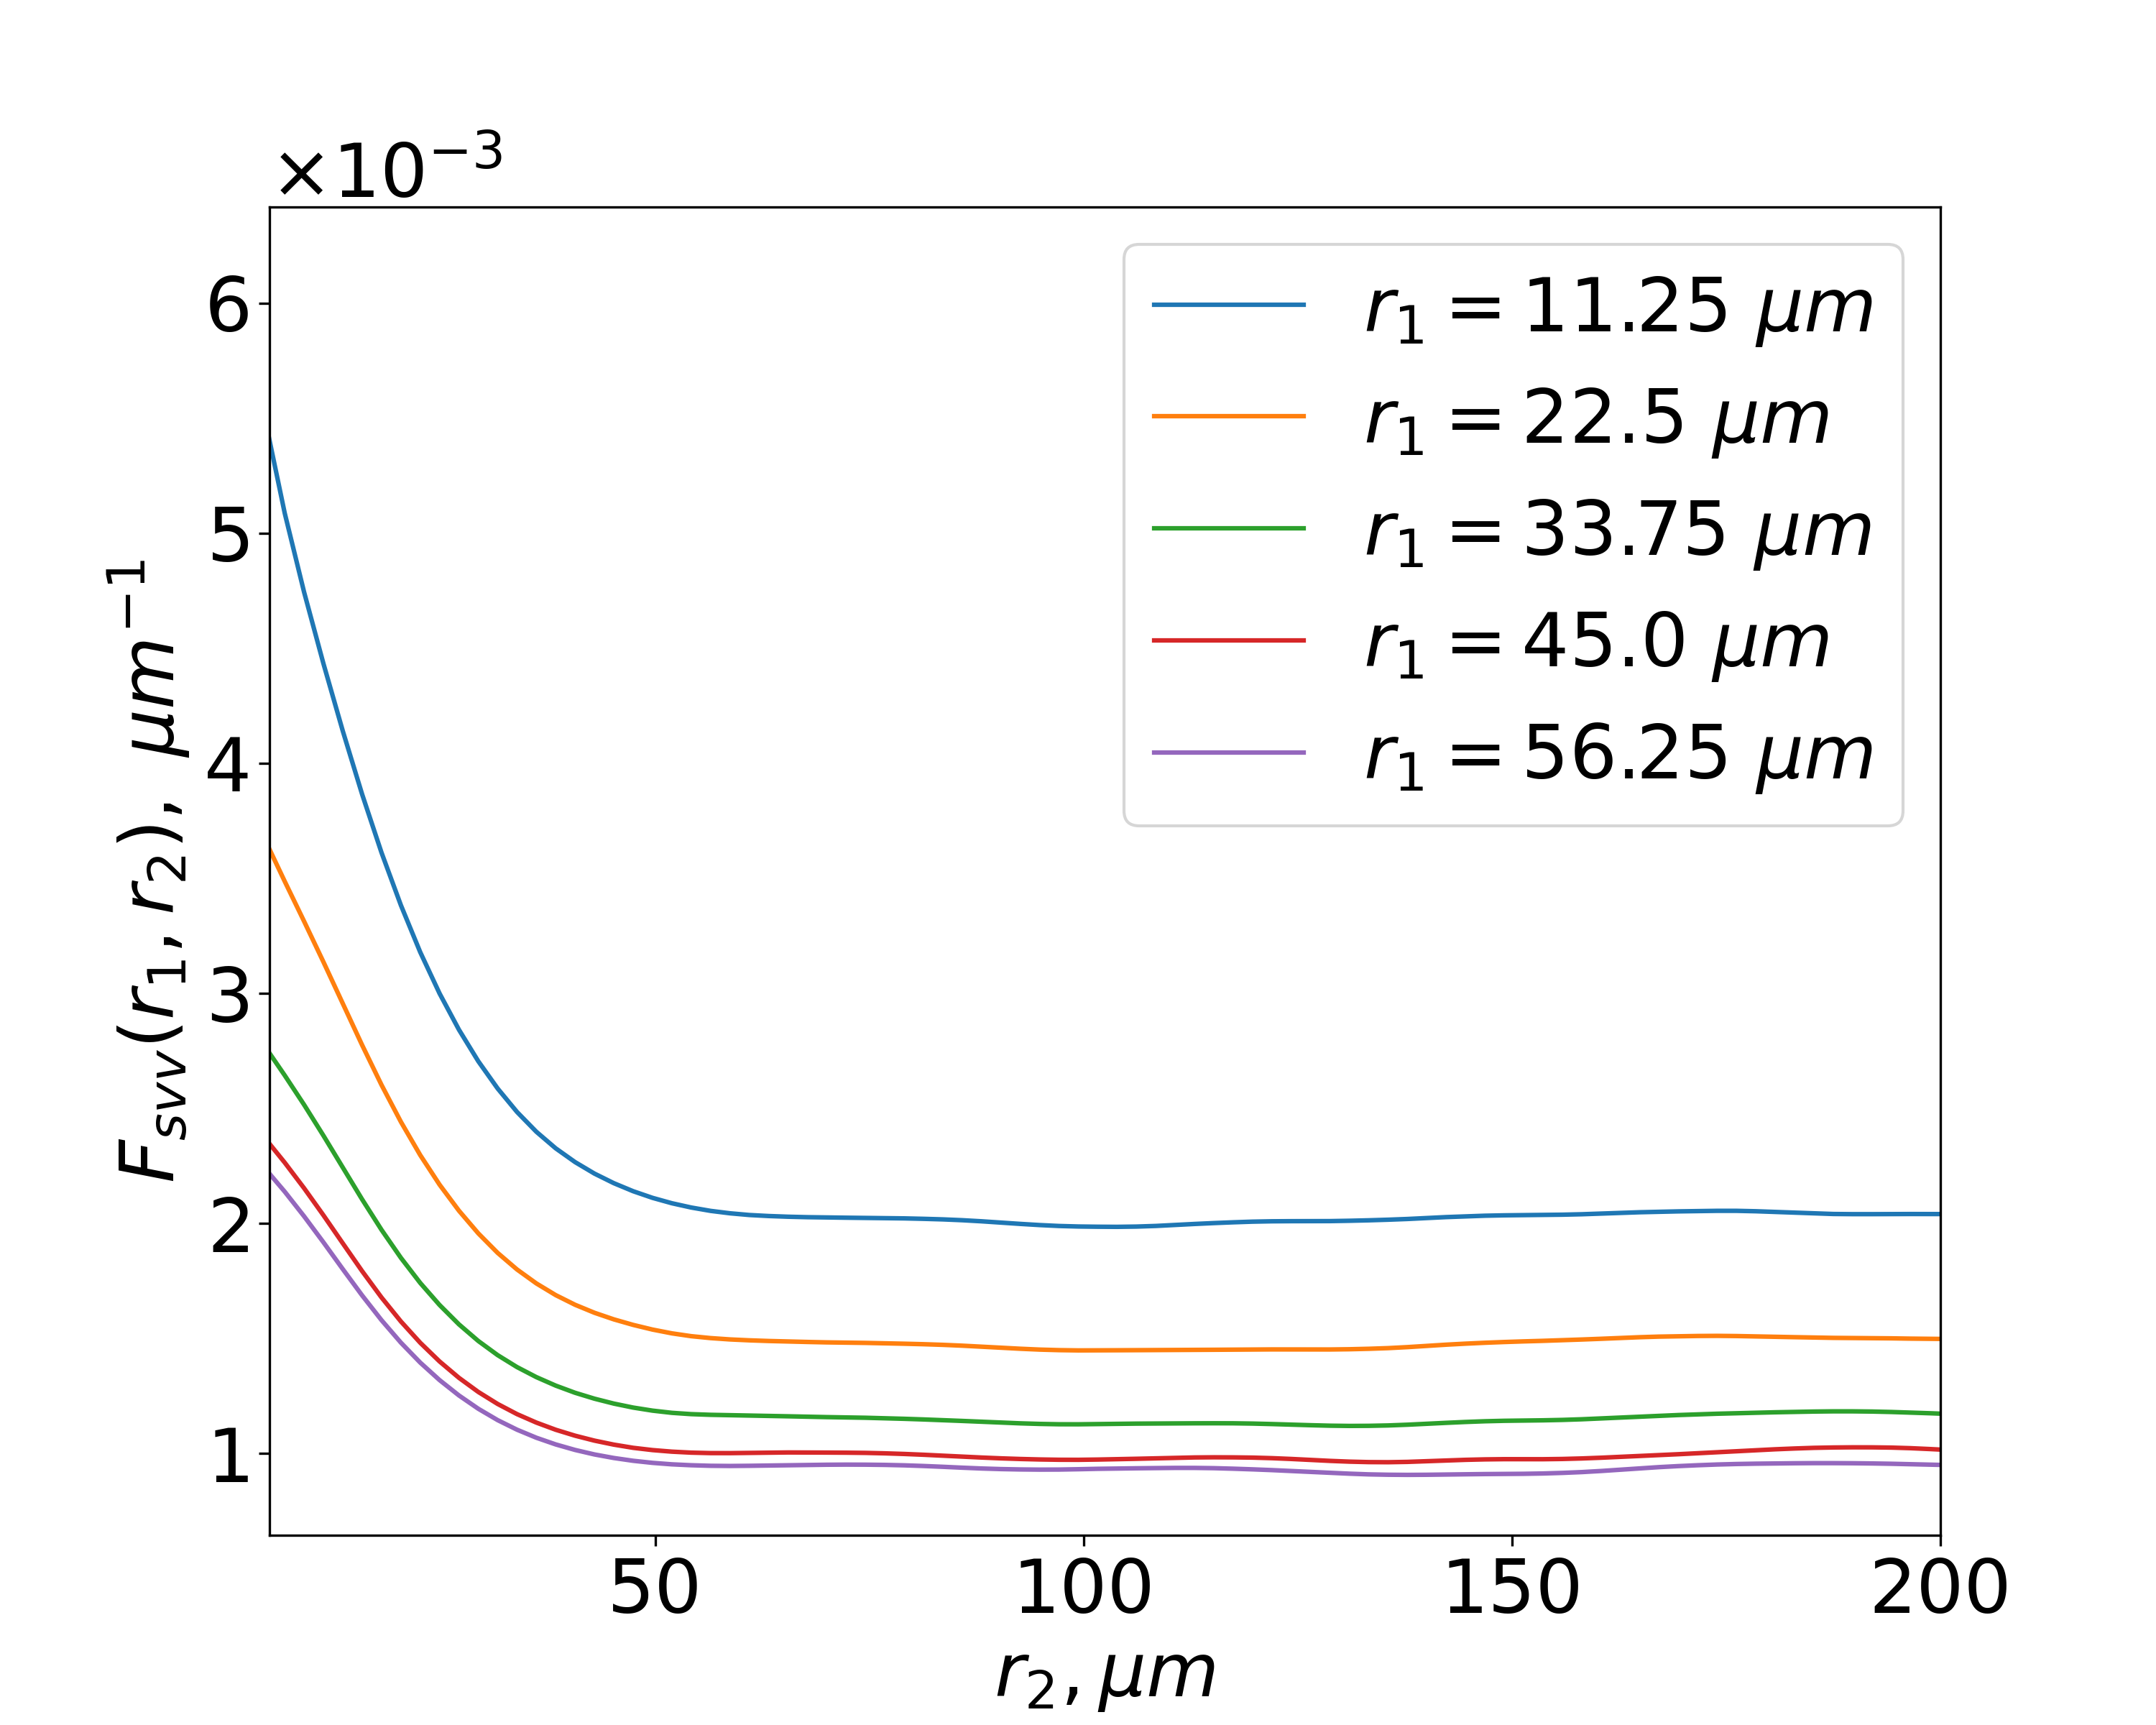
\includegraphics[width=0.4\linewidth]{images/15581-surfvoid2.png}
  \hfill
  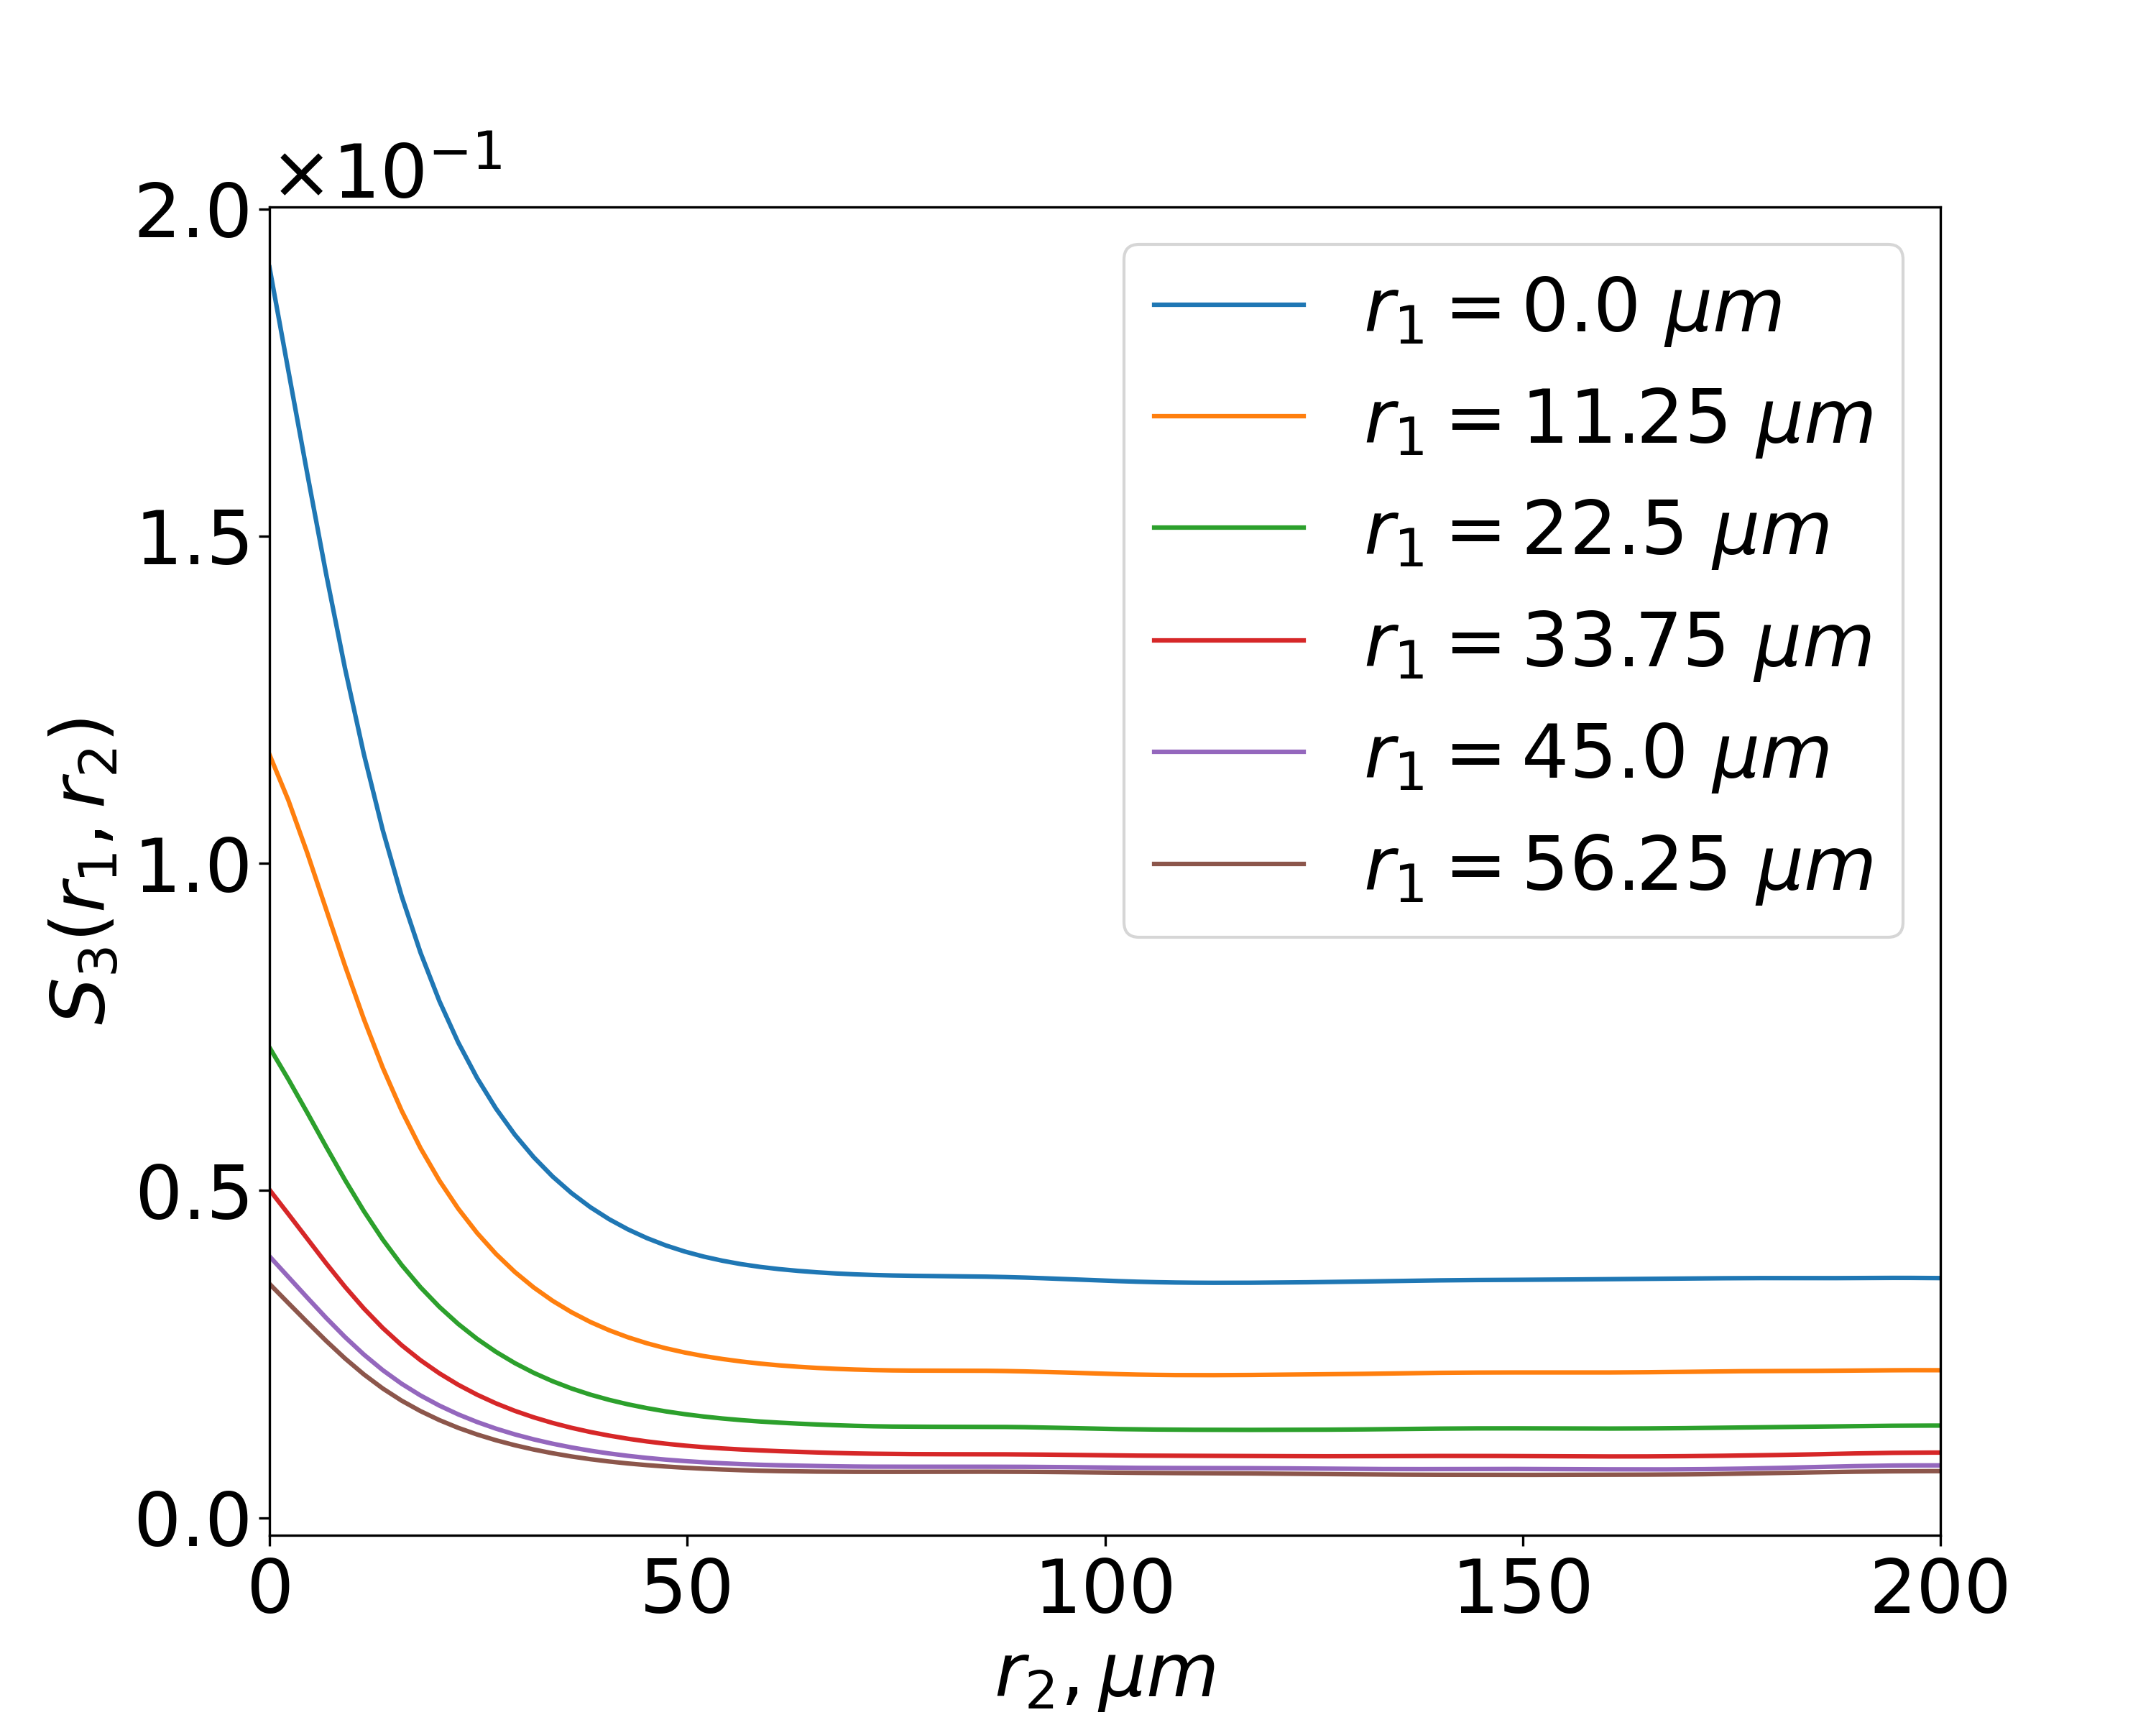
\includegraphics[width=0.4\linewidth]{images/15581-s3.png}
  \vskip\baselineskip
  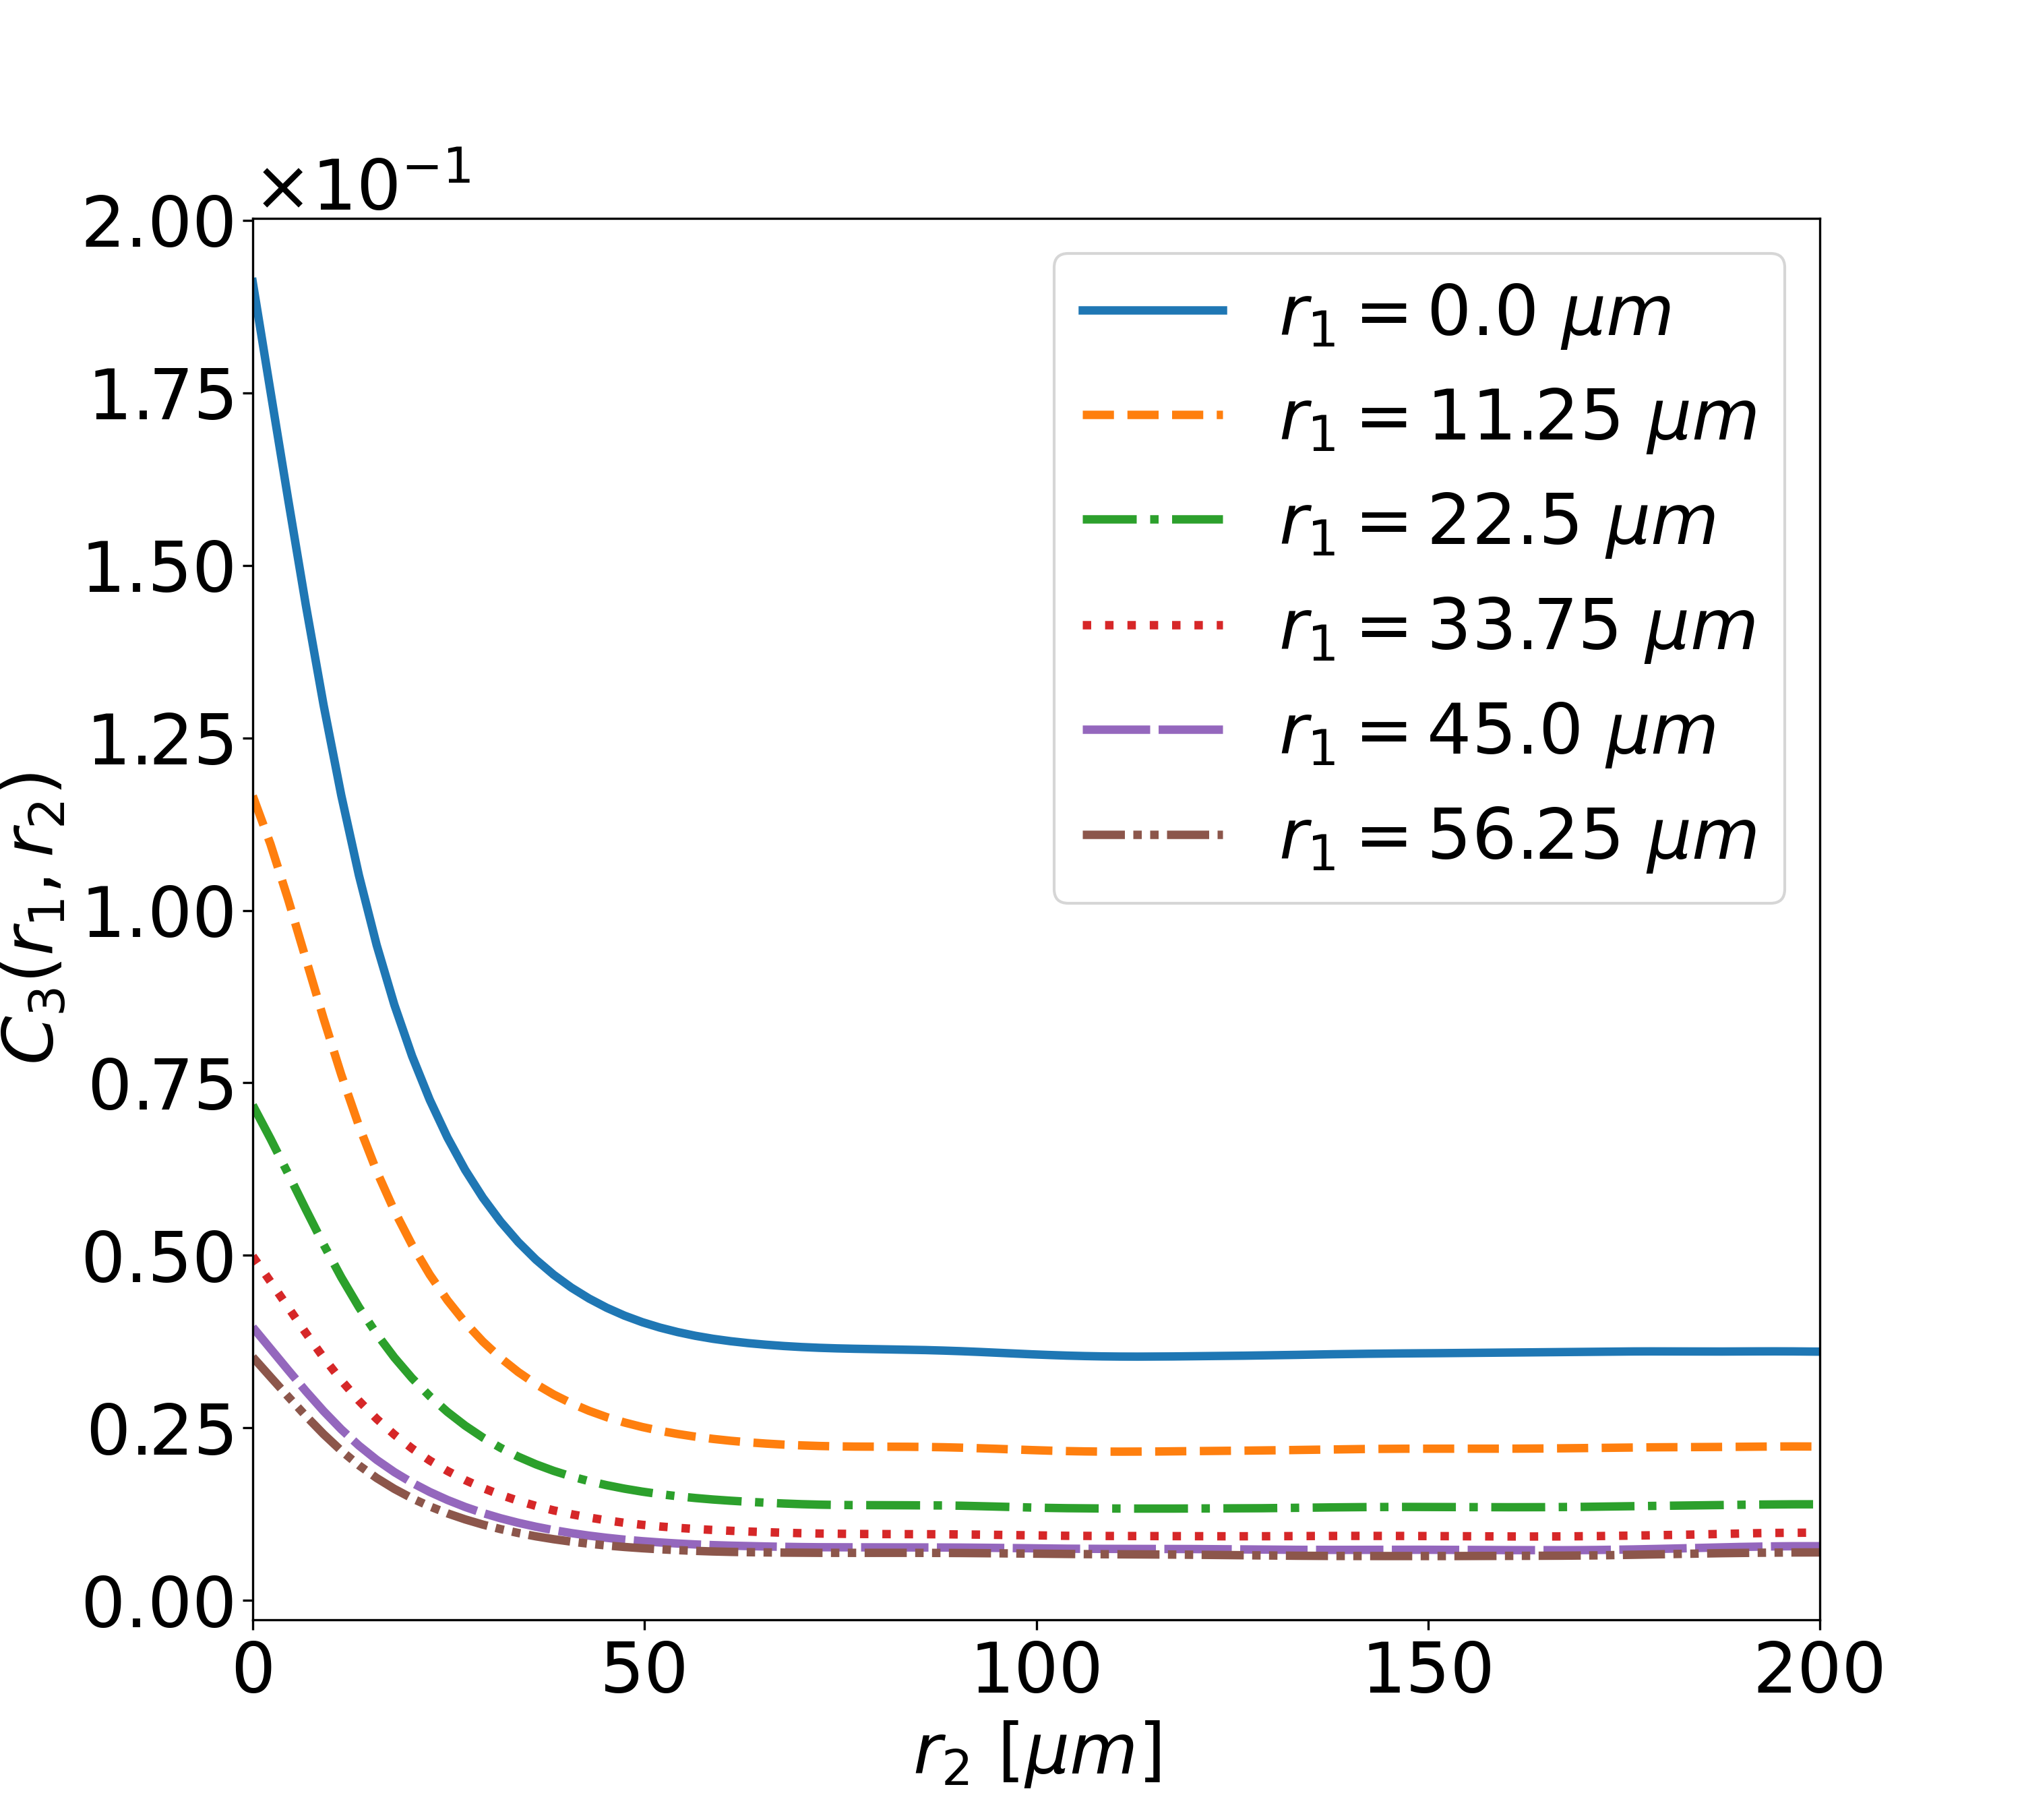
\includegraphics[width=0.4\linewidth]{images/15581-c3.png}
  \caption[]{Correlation functions for the sandstone XCT sample
    (\cref{fig:sample-sandstone-xct}).}
  \label{fig:sample-sandstone-xct-cf}
\end{figure*}

\begin{figure*}[tp]
  \centering
  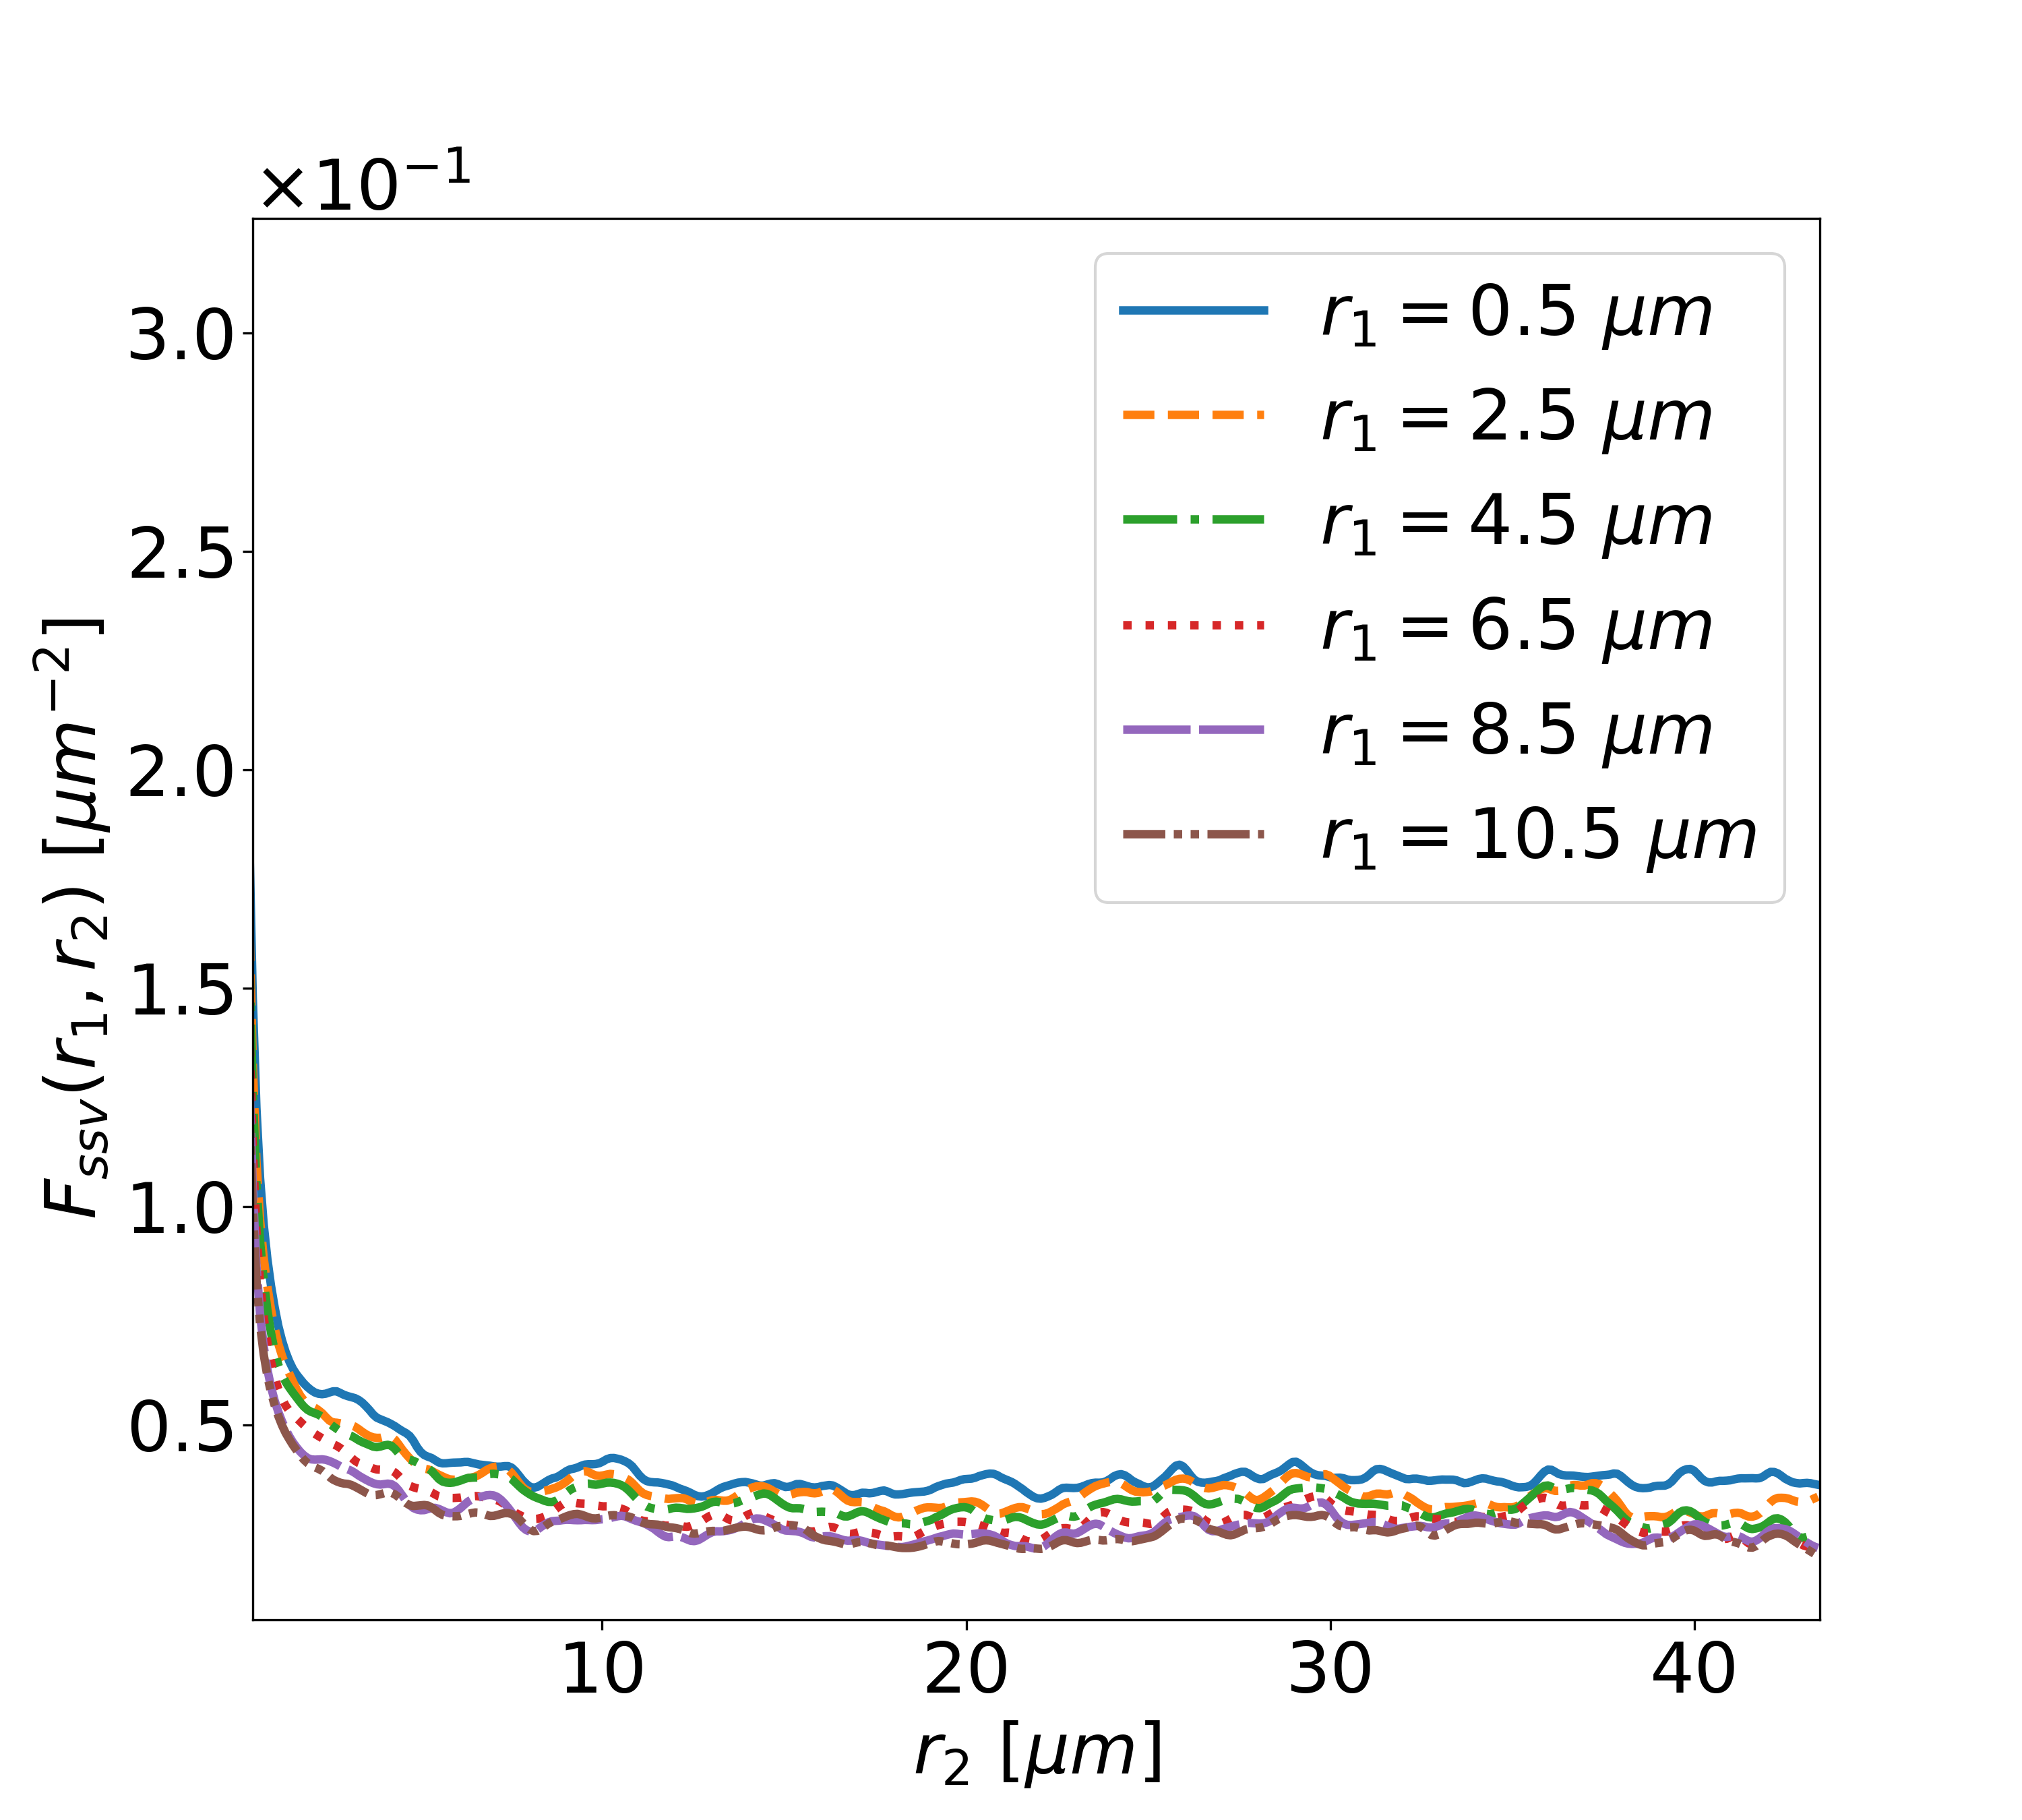
\includegraphics[width=0.4\linewidth]{images/sandstone1.png-surf2void.png}
  \hfill
  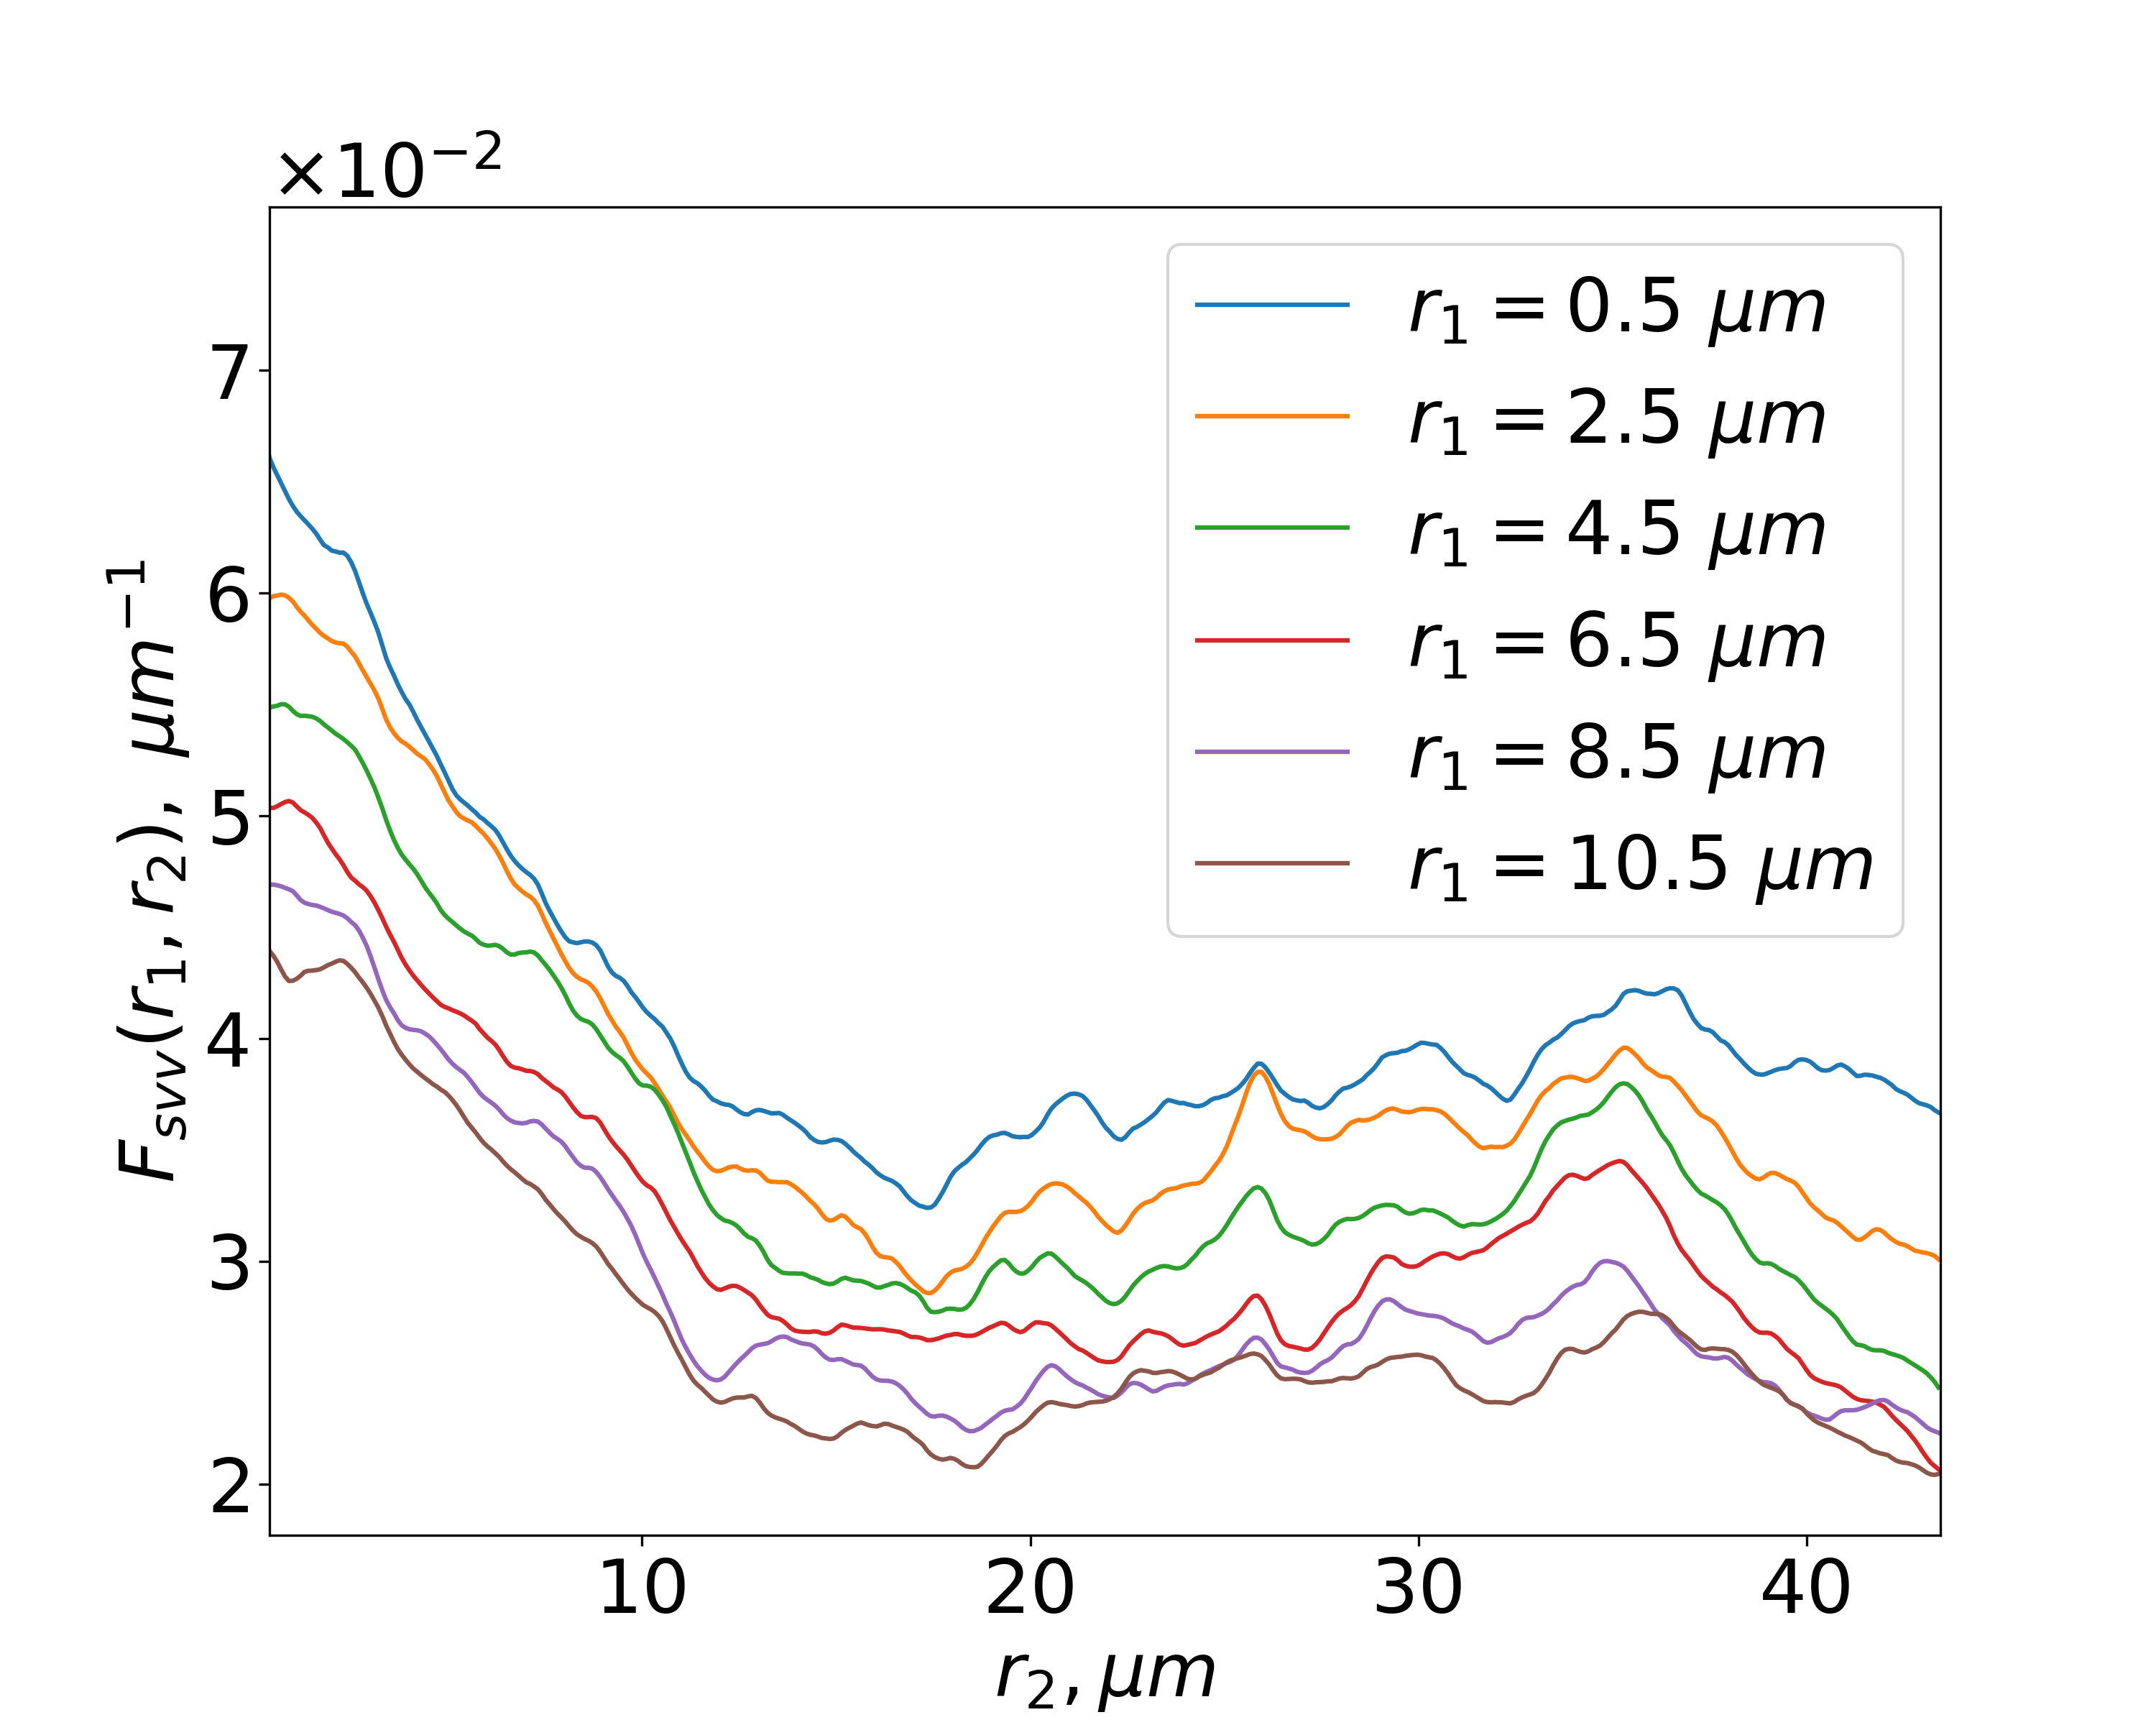
\includegraphics[width=0.4\linewidth]{images/sandstone1.png-surfvoid2.png}
  \vskip\baselineskip
  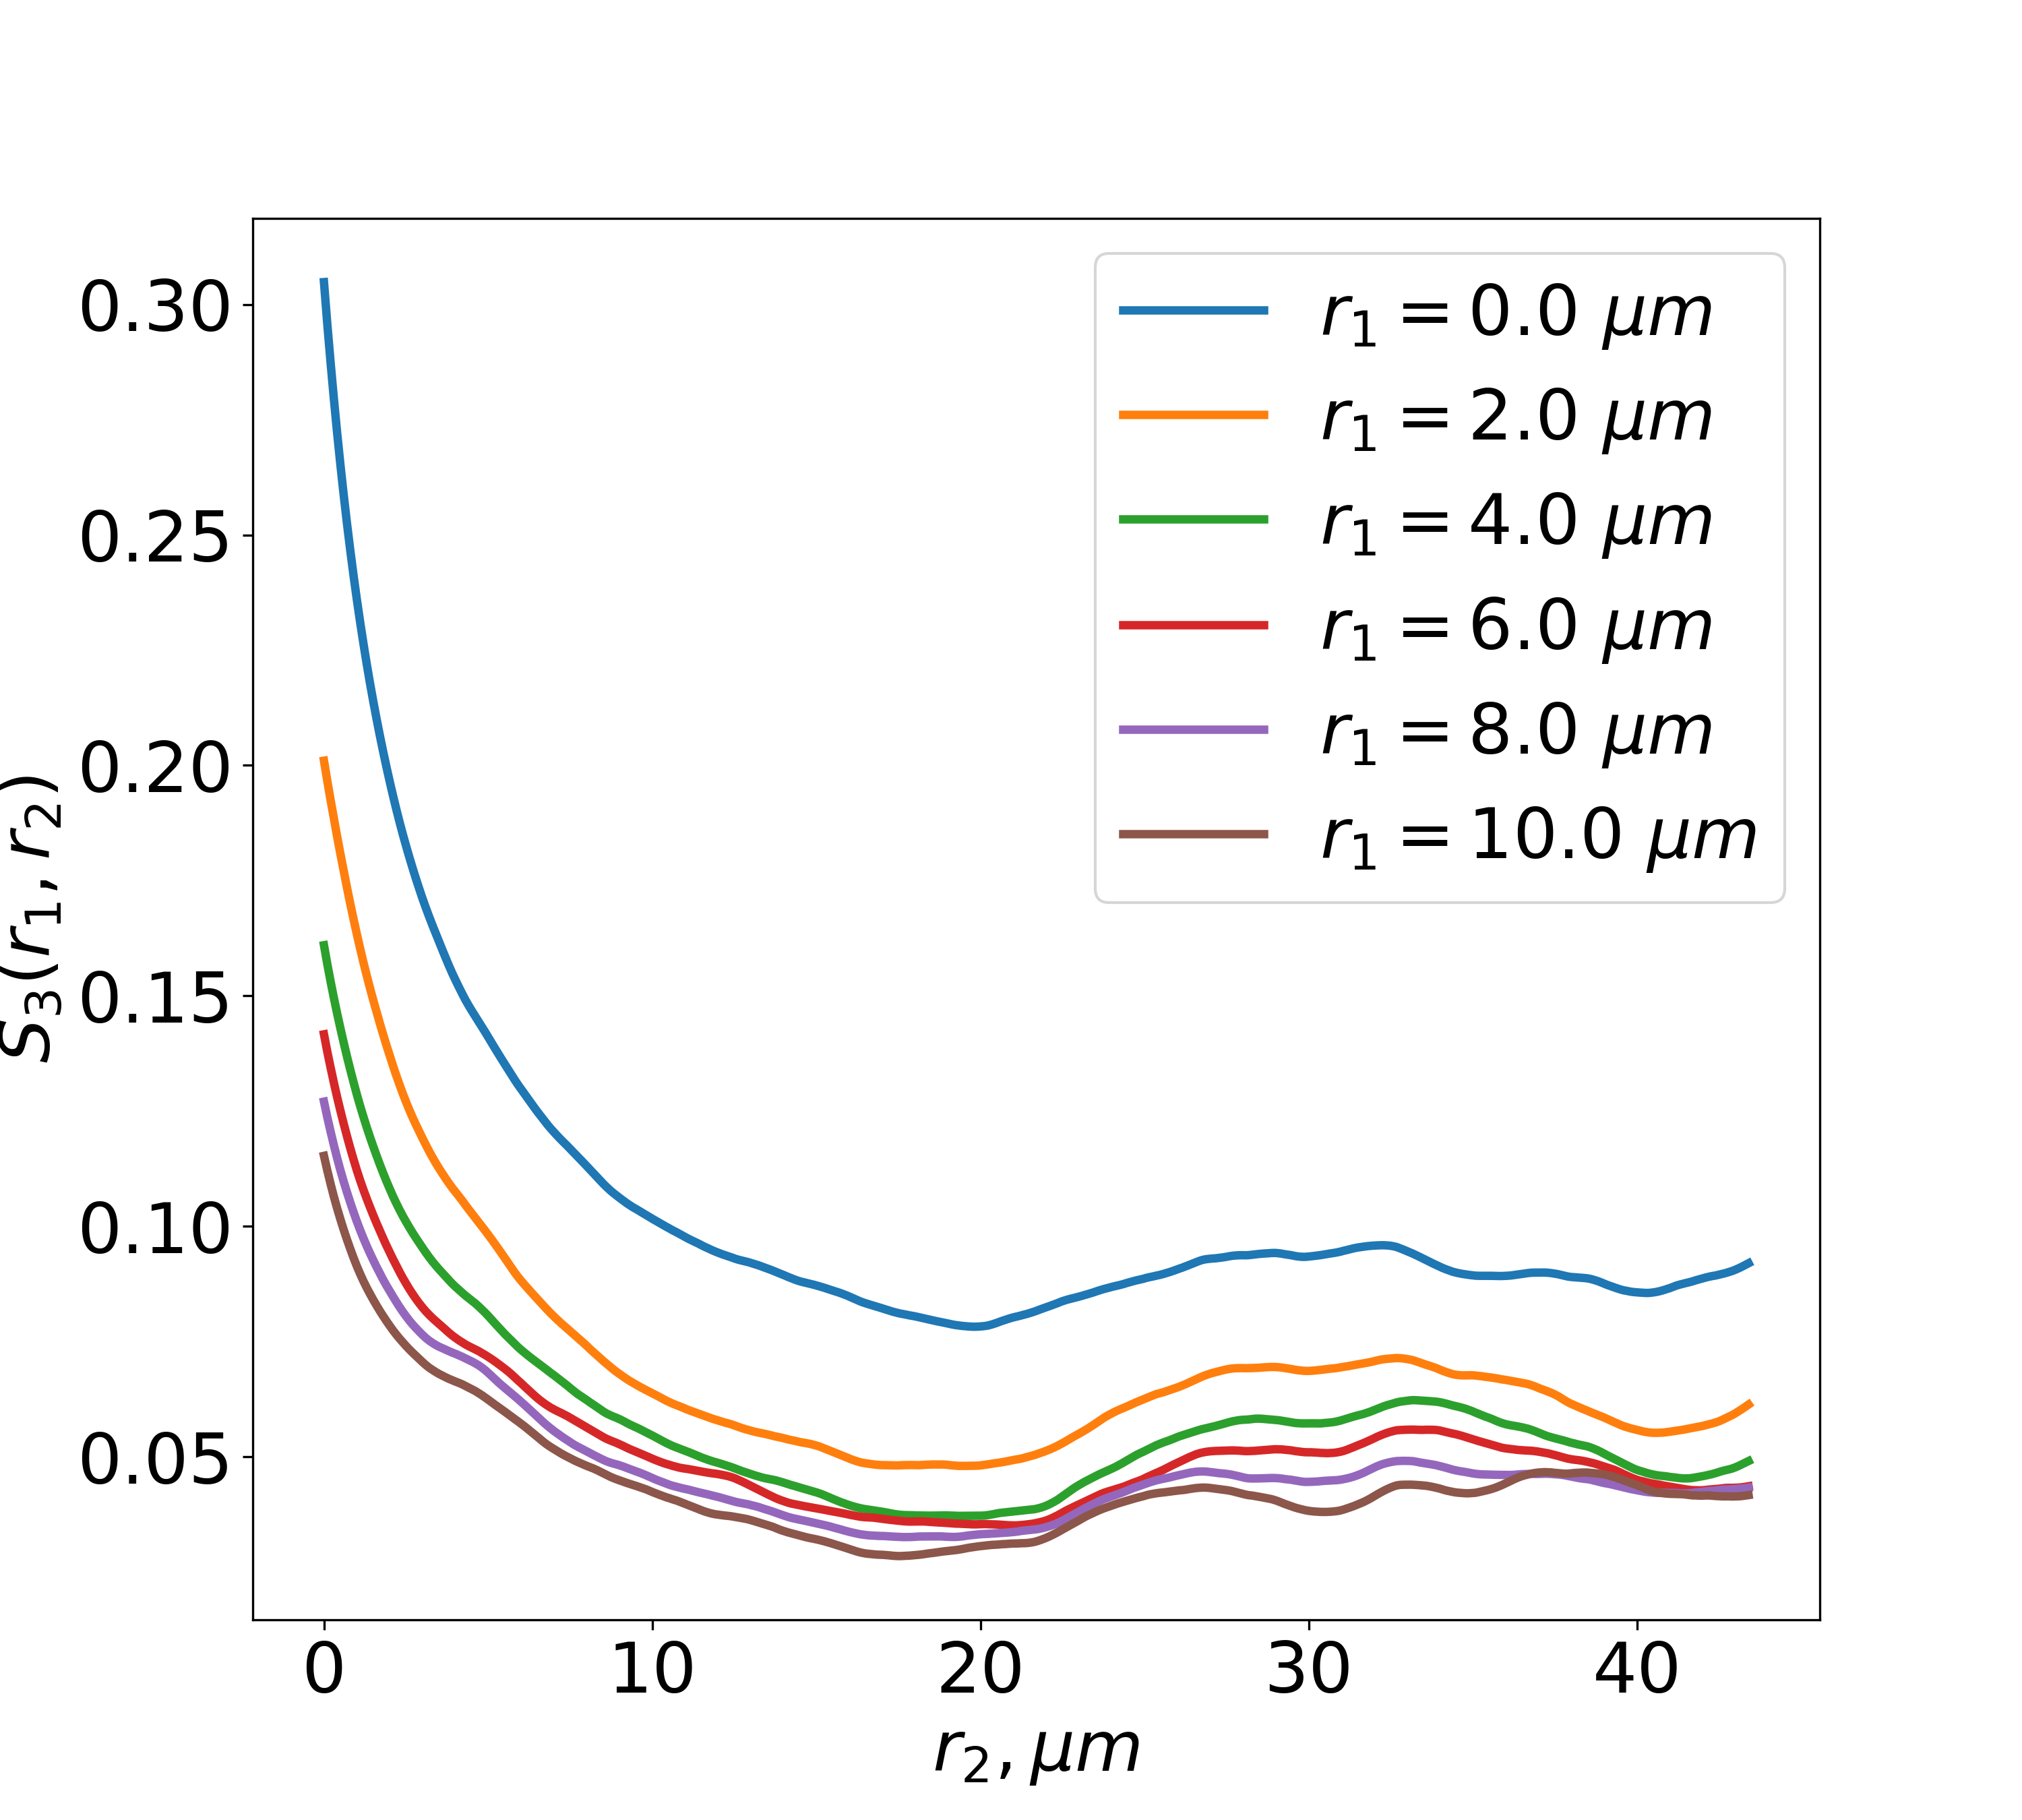
\includegraphics[width=0.4\linewidth]{images/sandstone1.png-s3.png}
  \hfill
  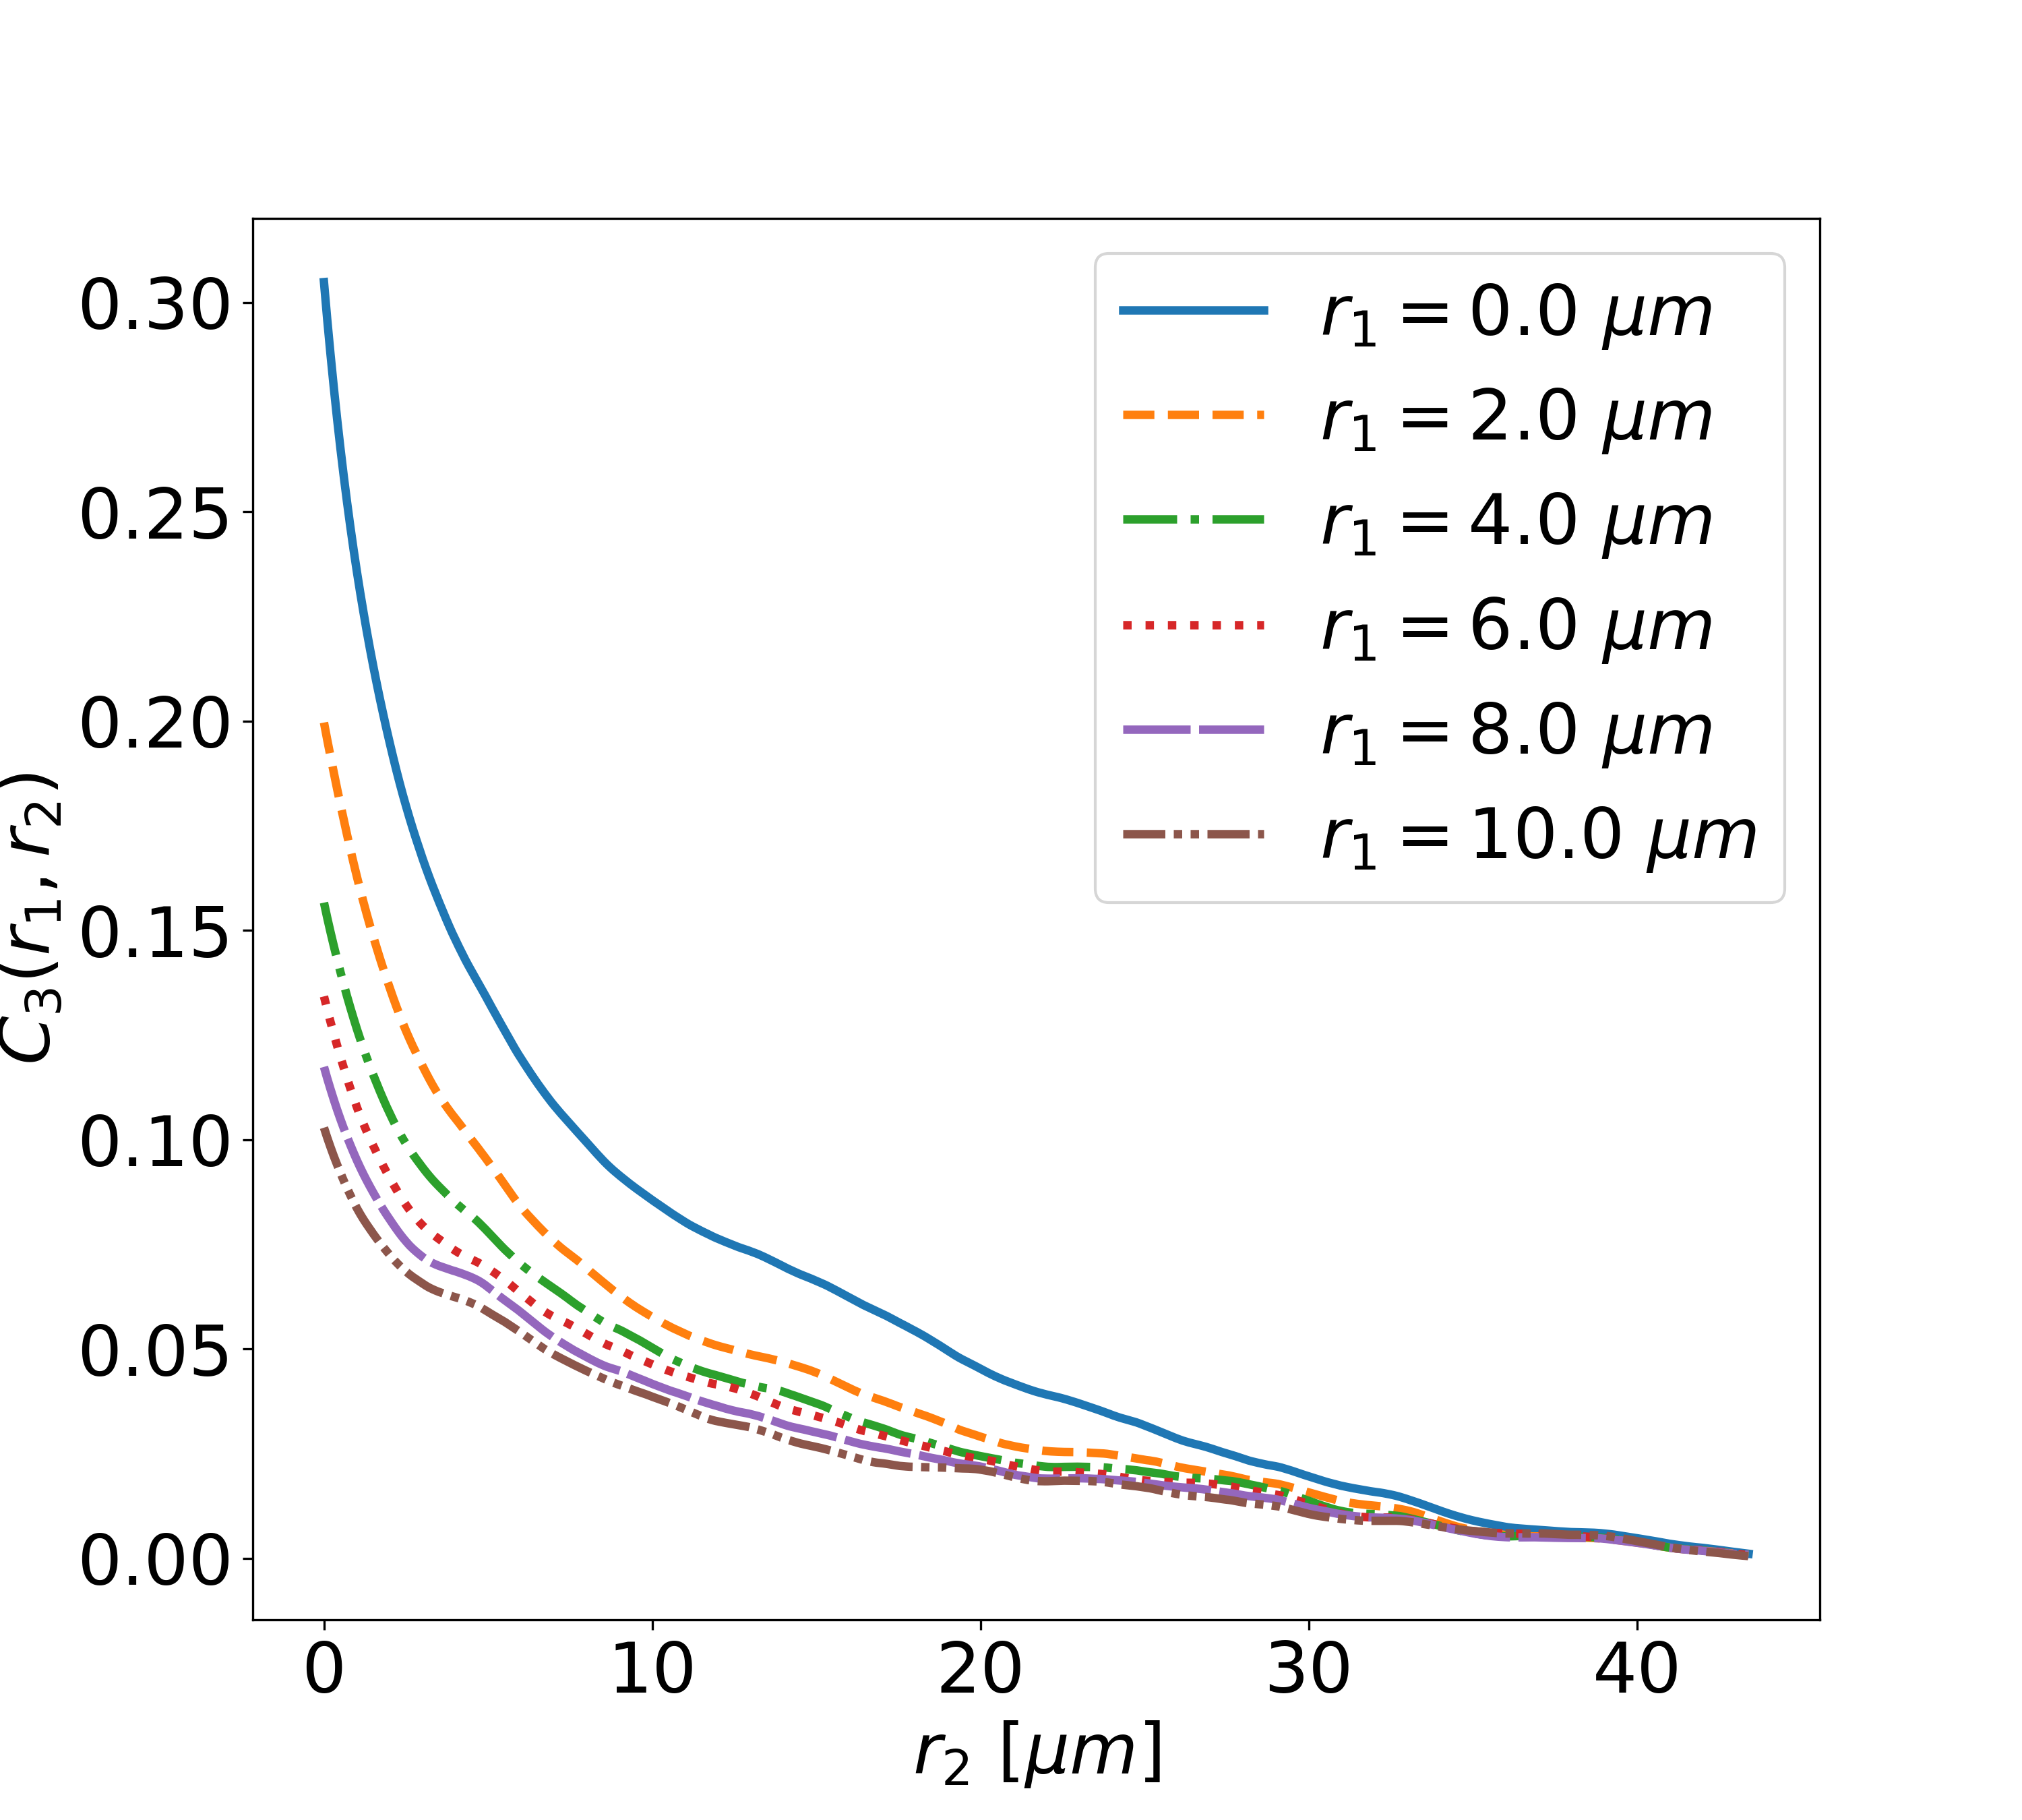
\includegraphics[width=0.4\linewidth]{images/sandstone1.png-c3.png}
  \caption[]{Correlation functions for the sandstone SEM sample
    (\cref{fig:sample-sandstone}).}
  \label{fig:sample-sandstone-cf}
\end{figure*}

\begin{figure*}[tp]
  \centering
  \subfigure[Soil]{
    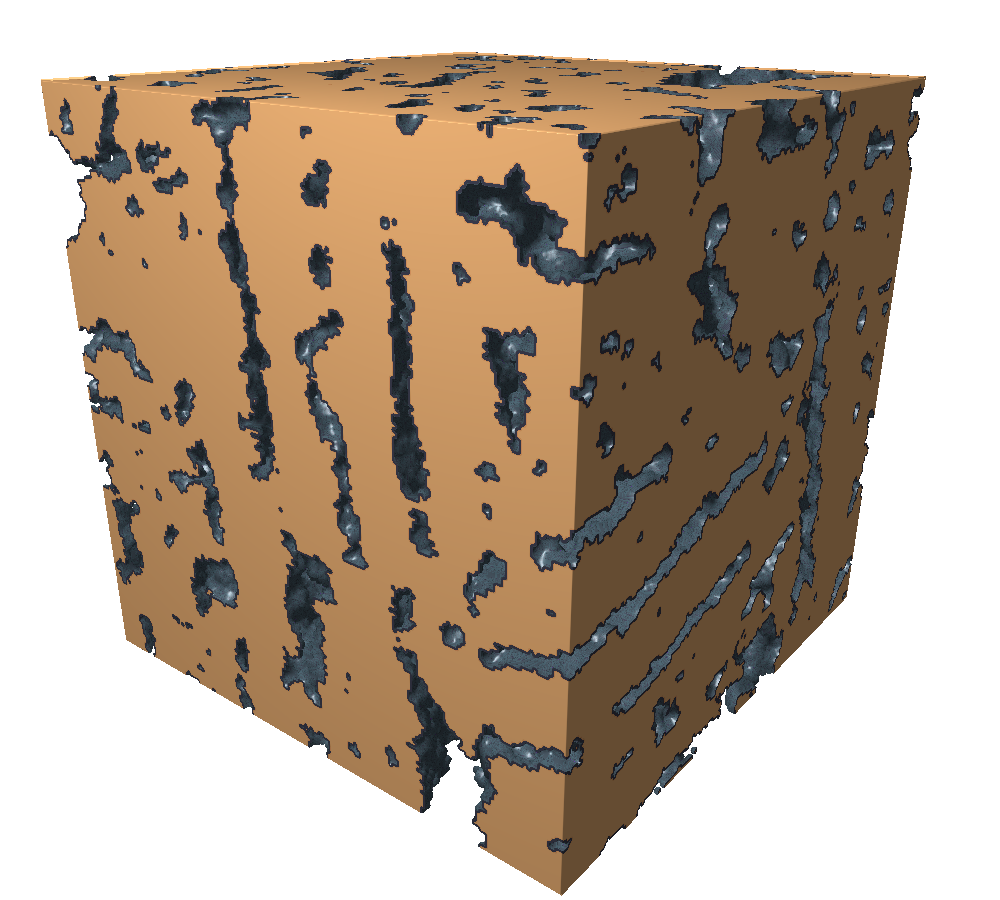
\includegraphics[width=0.4\linewidth]{images/soil-rot.png}}
  \hfill
  \subfigure[Shale]{
    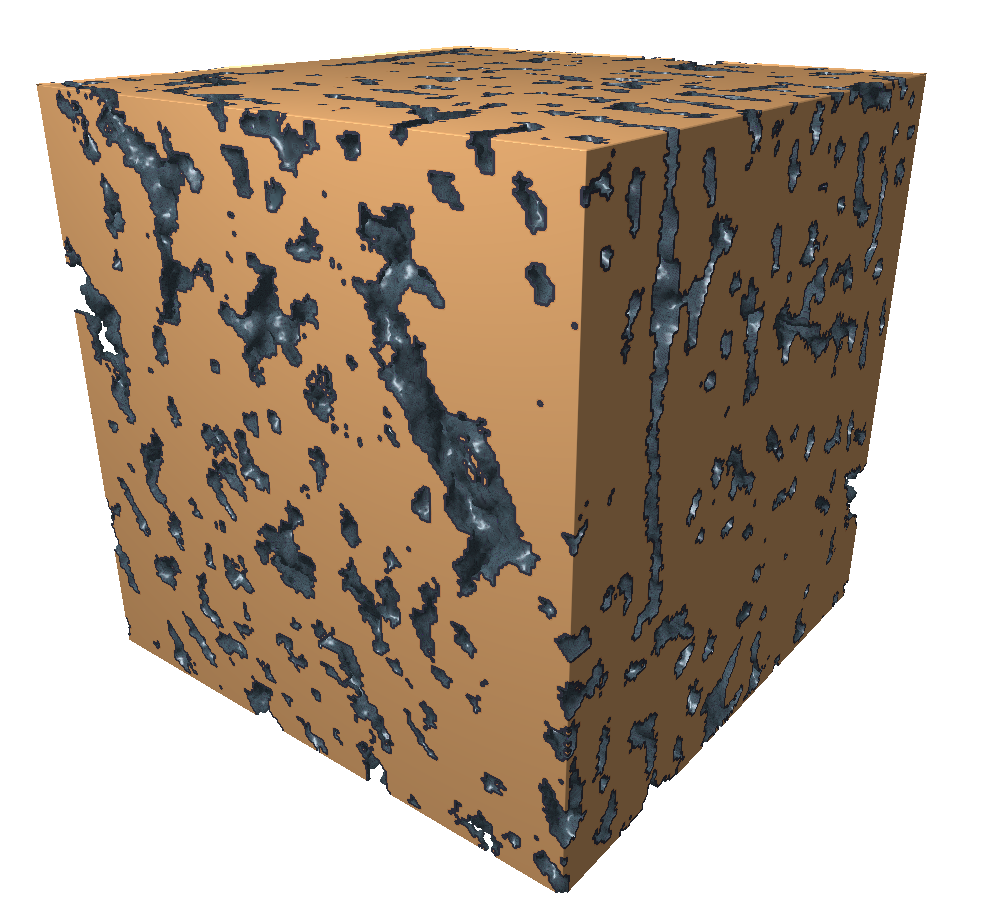
\includegraphics[width=0.4\linewidth]{images/shale-rot.png}}
  \caption[]{Rotations of anisotropic samples with pores aligned with the
    coordinate axes.}
  \label{fig:samples-rot}
\end{figure*}

\begin{figure*}[tp]
  \centering
  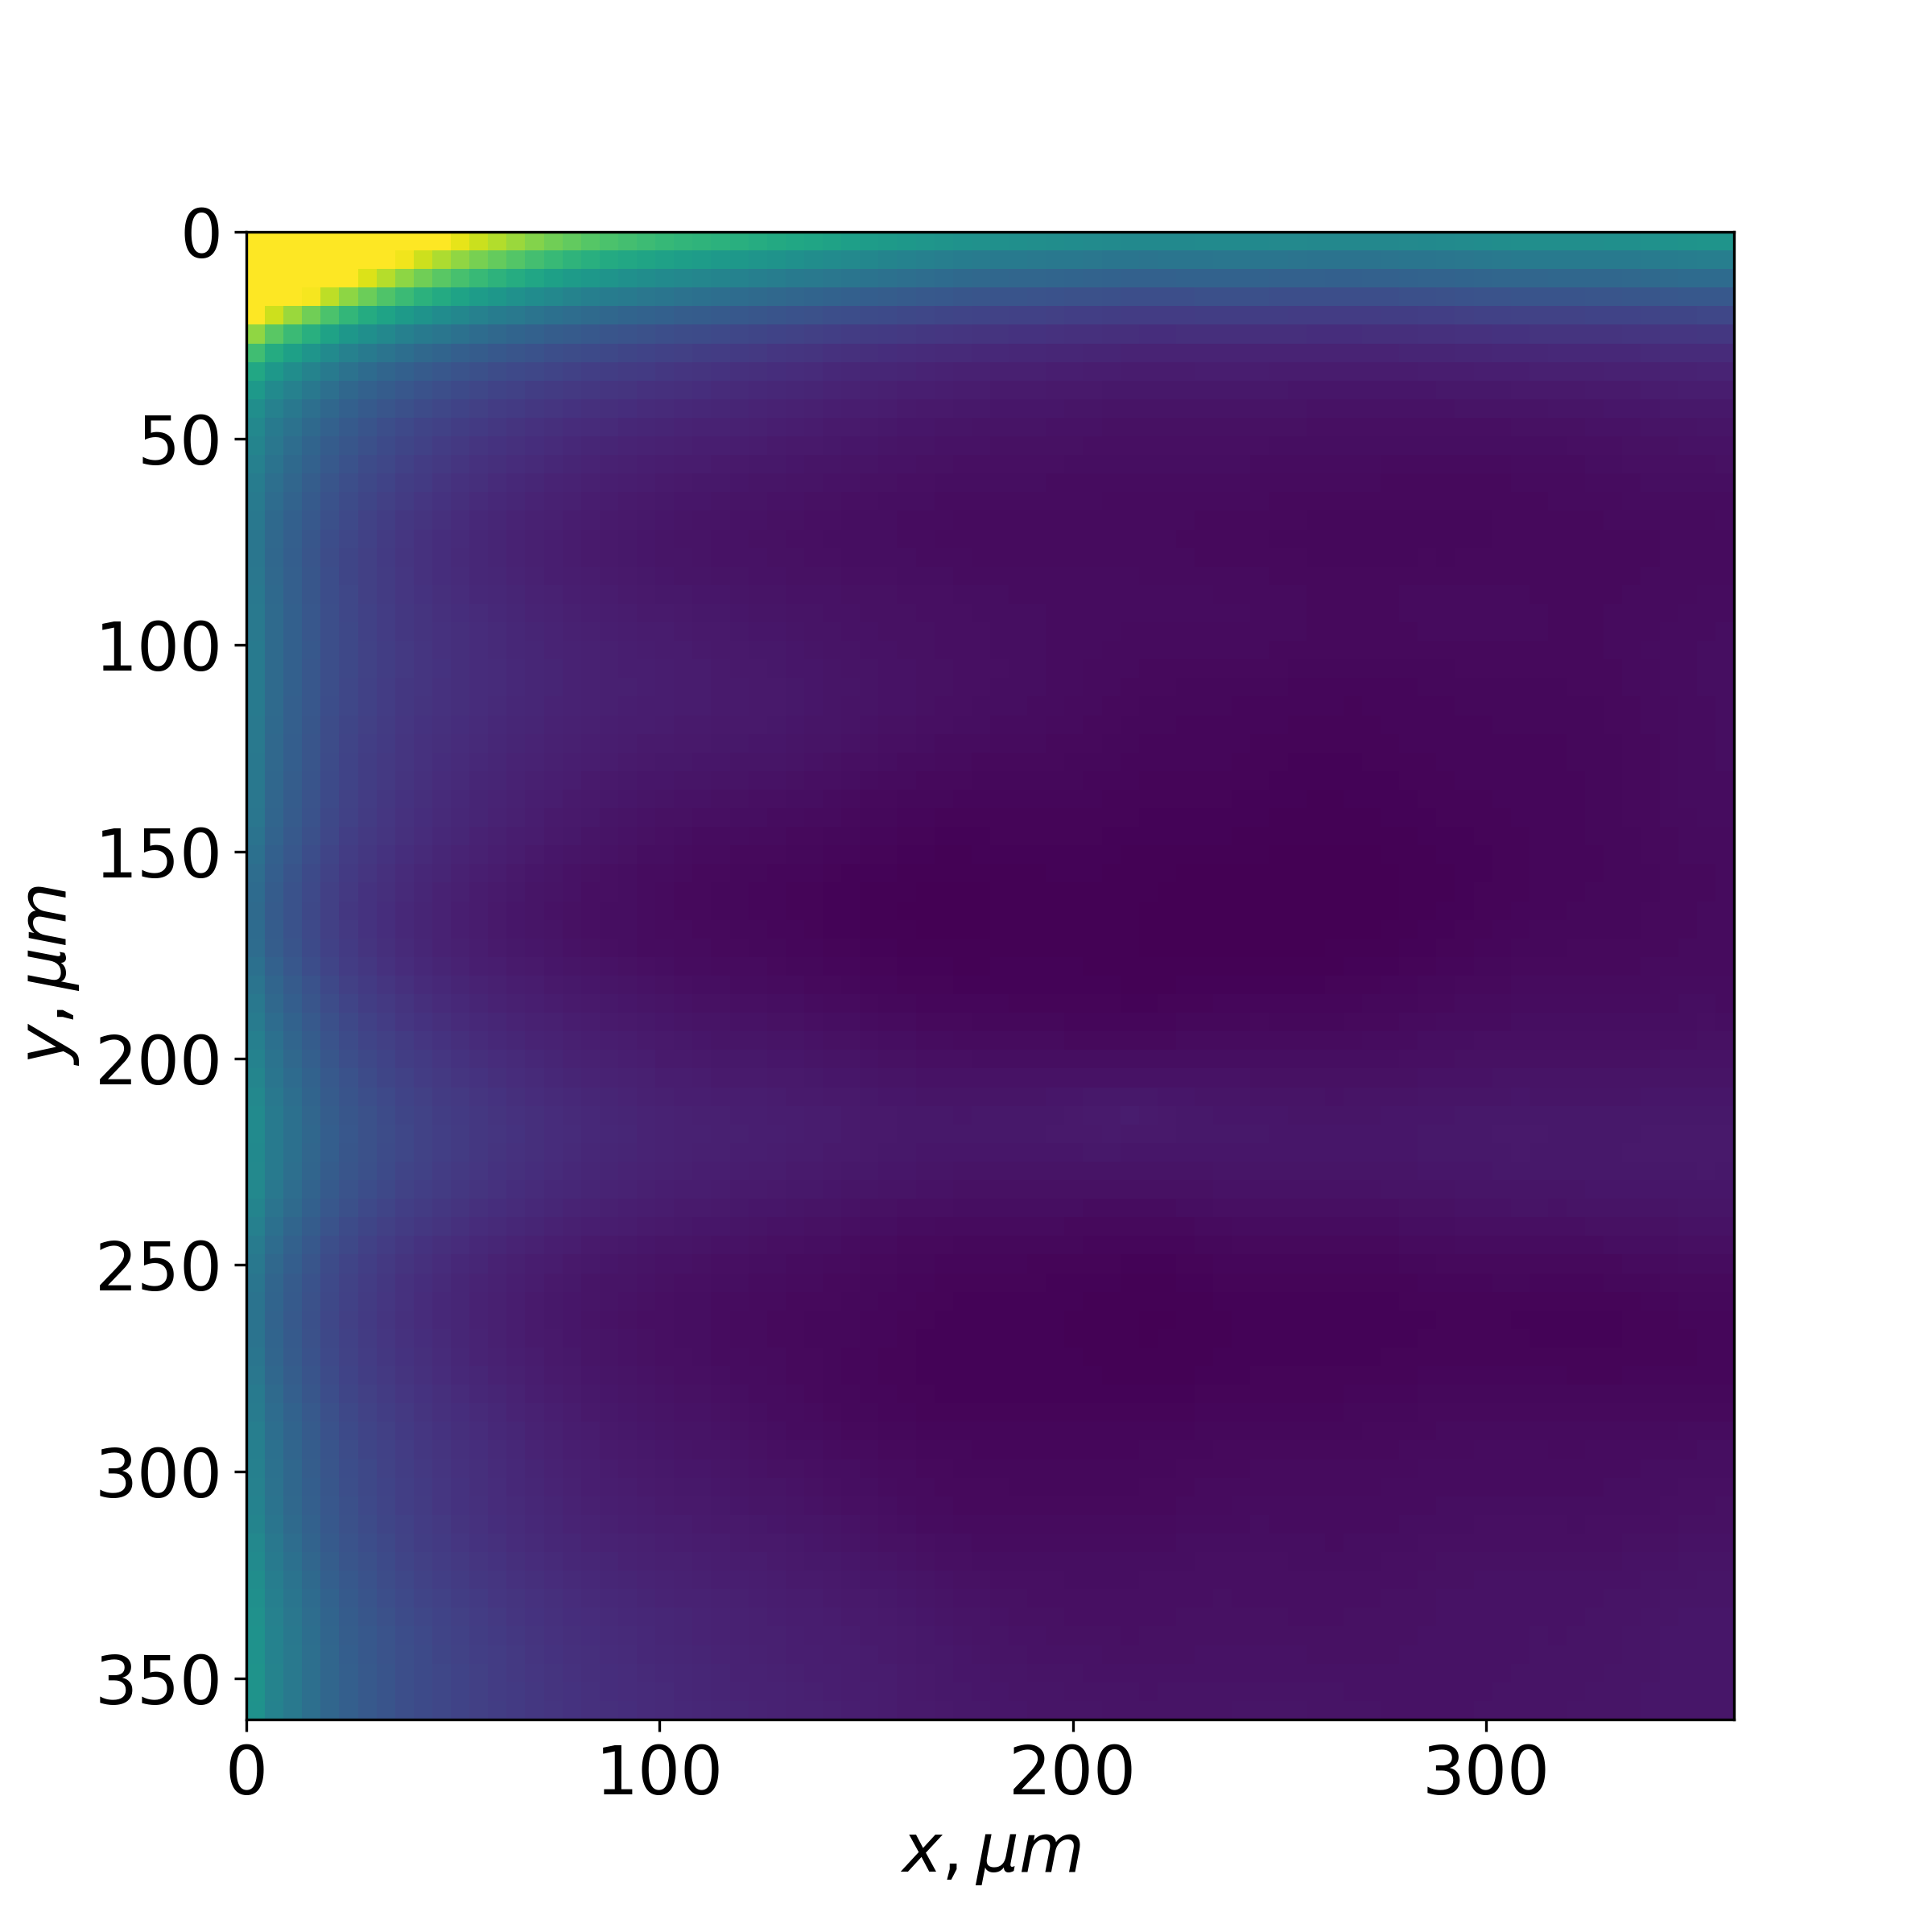
\includegraphics[width=0.4\linewidth]{images/soil-s3.png}
  \hfill
  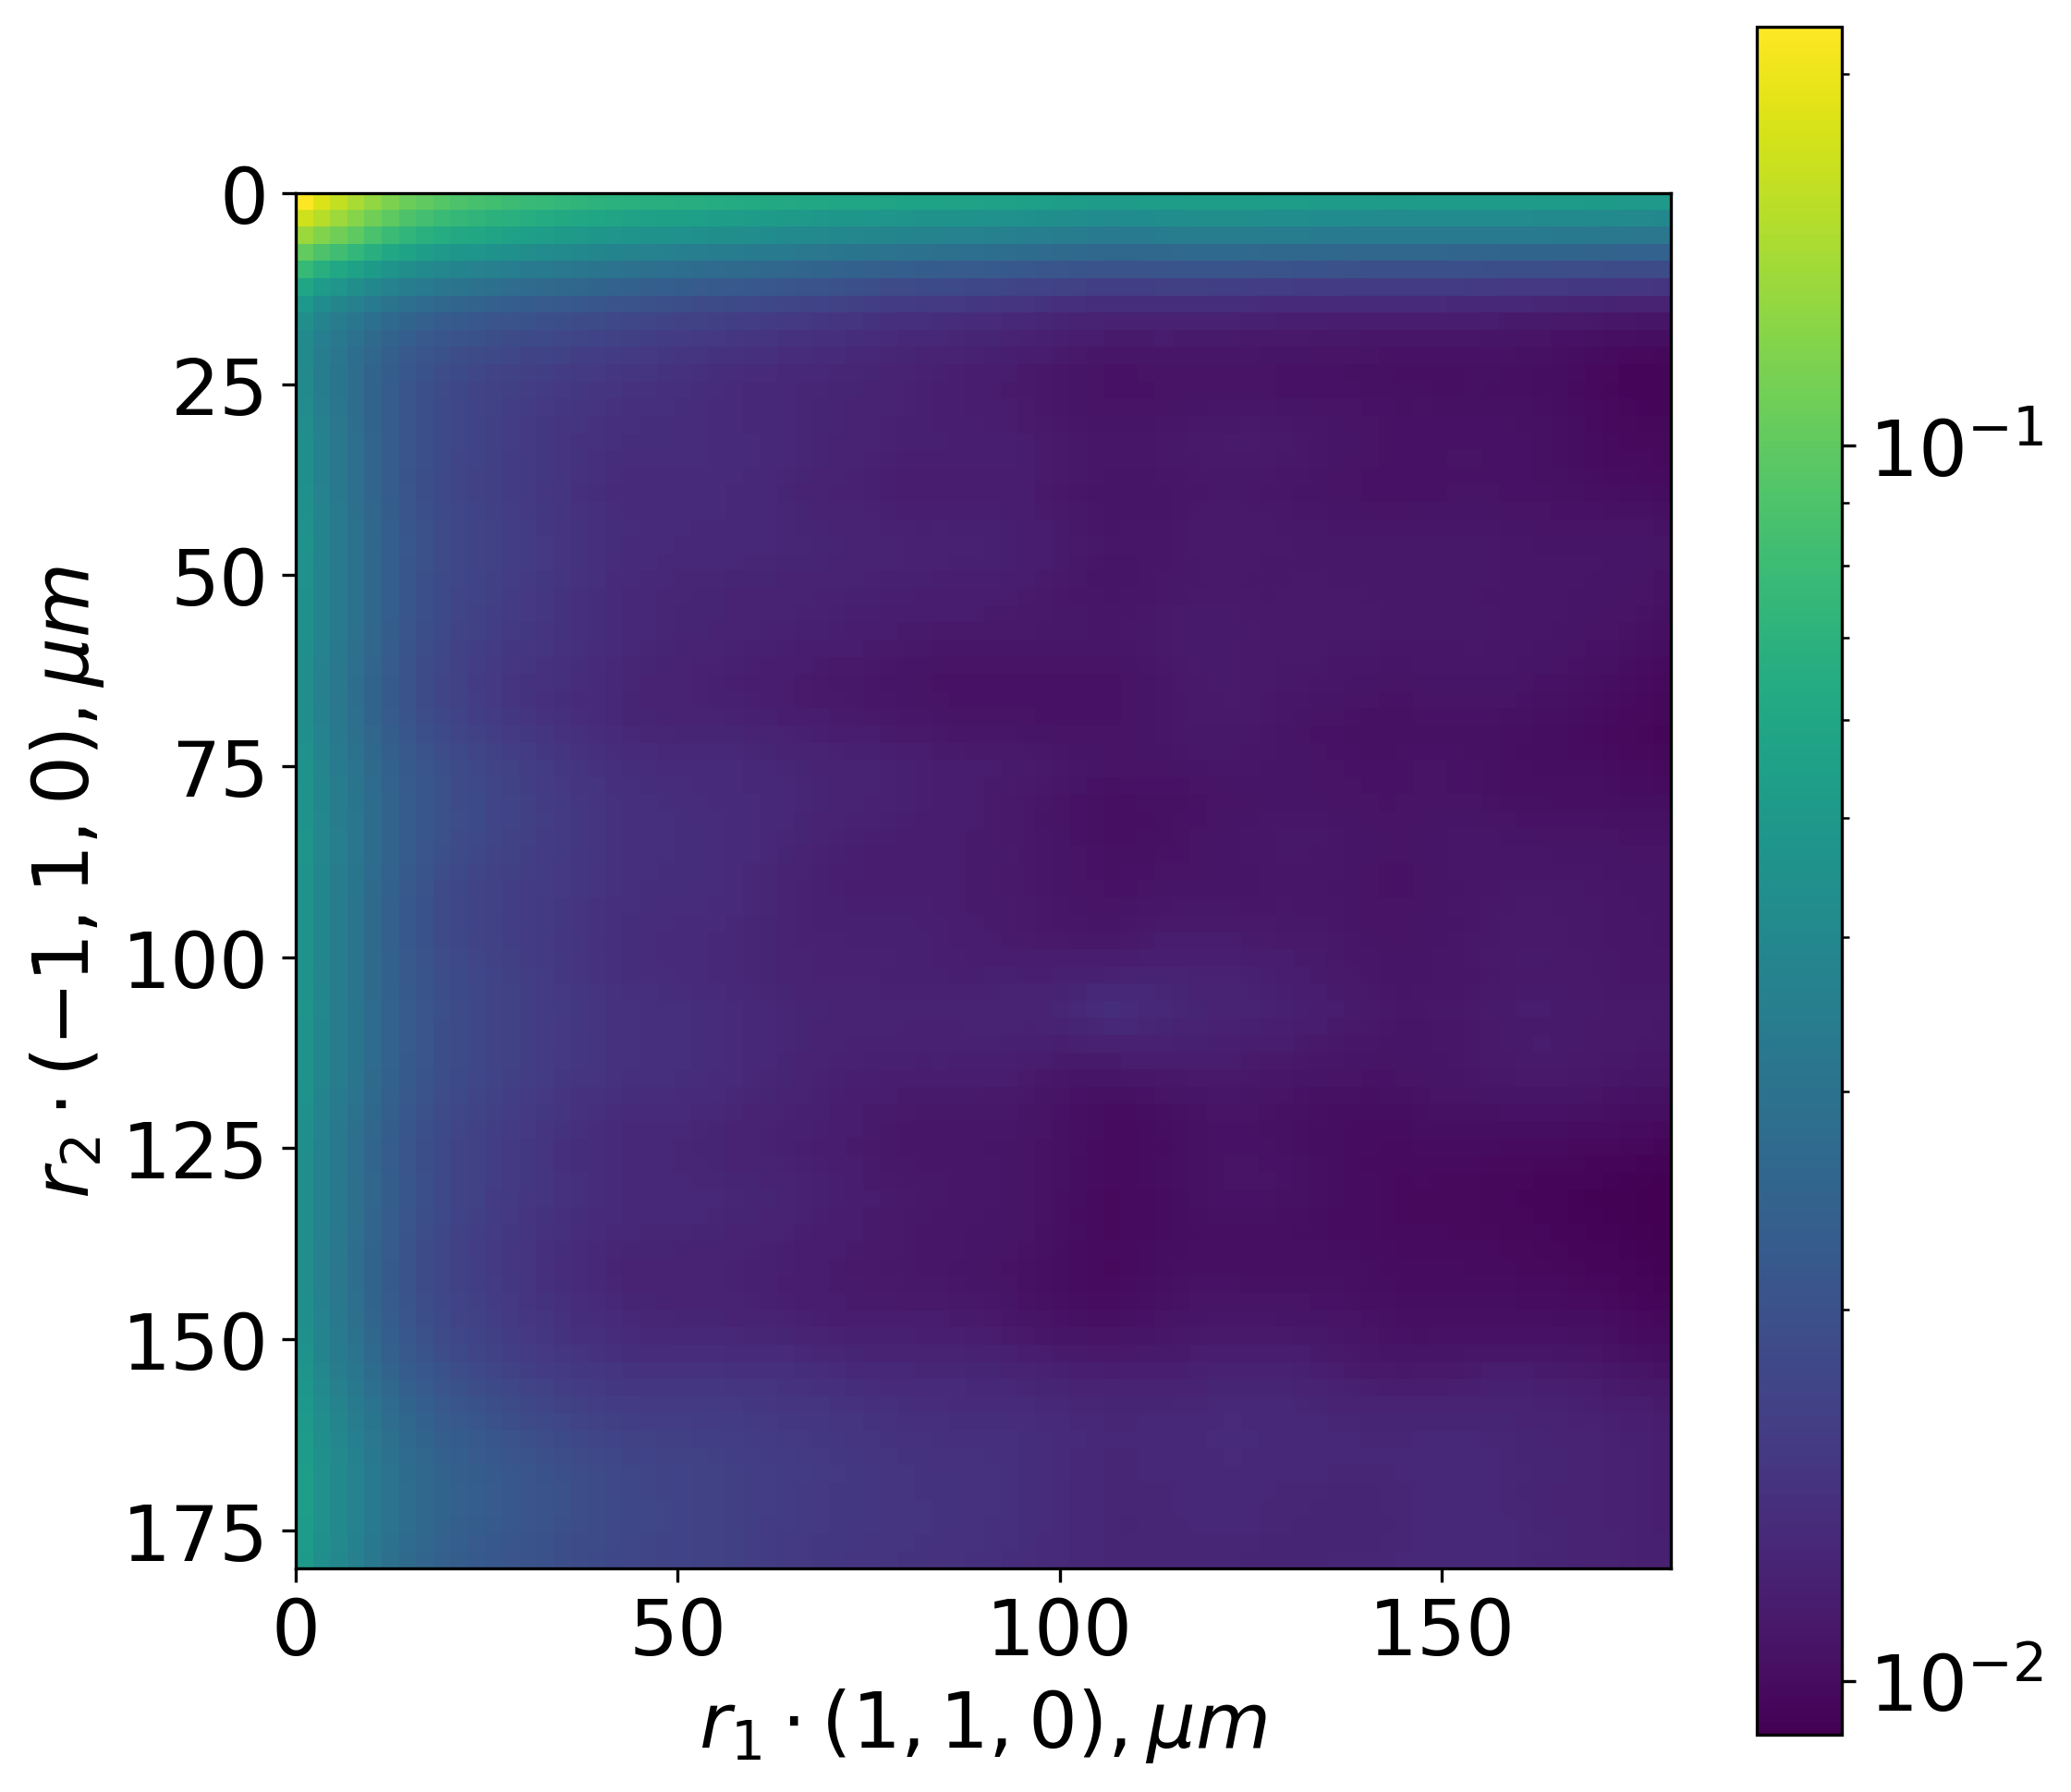
\includegraphics[width=0.4\linewidth]{images/shale-s3.png}
  \vskip\baselineskip
  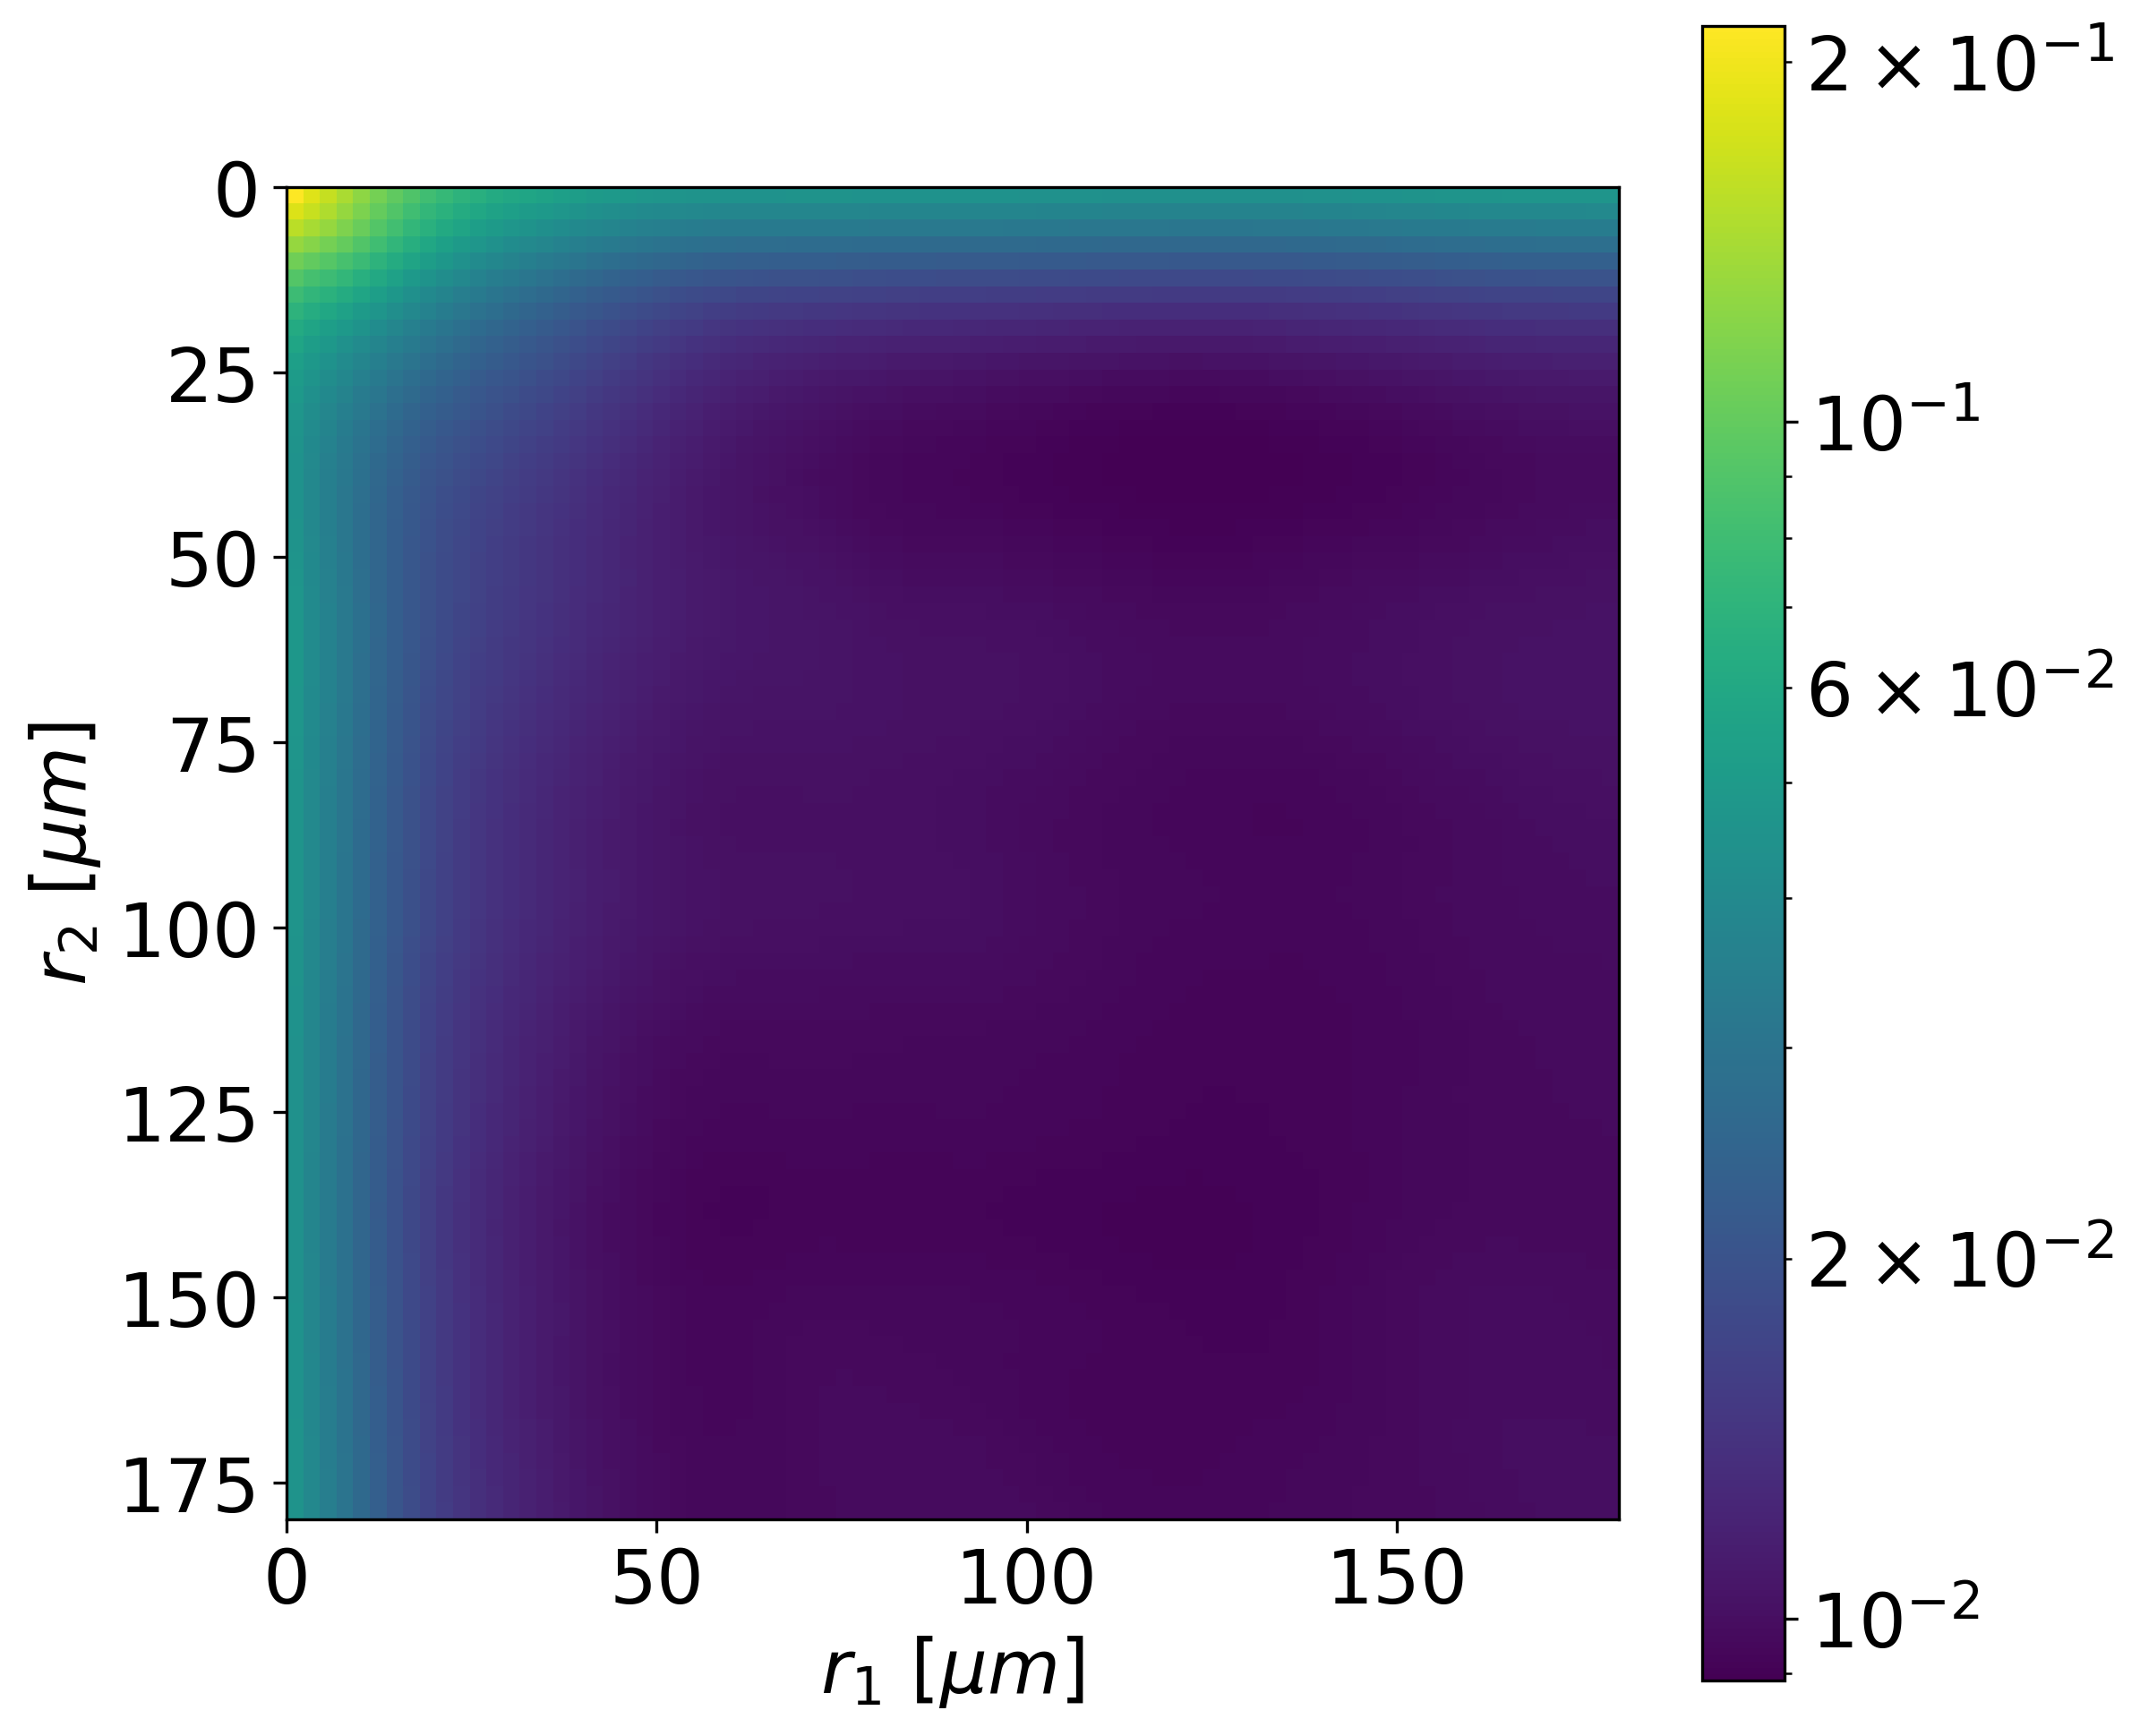
\includegraphics[width=0.4\linewidth]{images/soil-avg.png}
  \hfill
  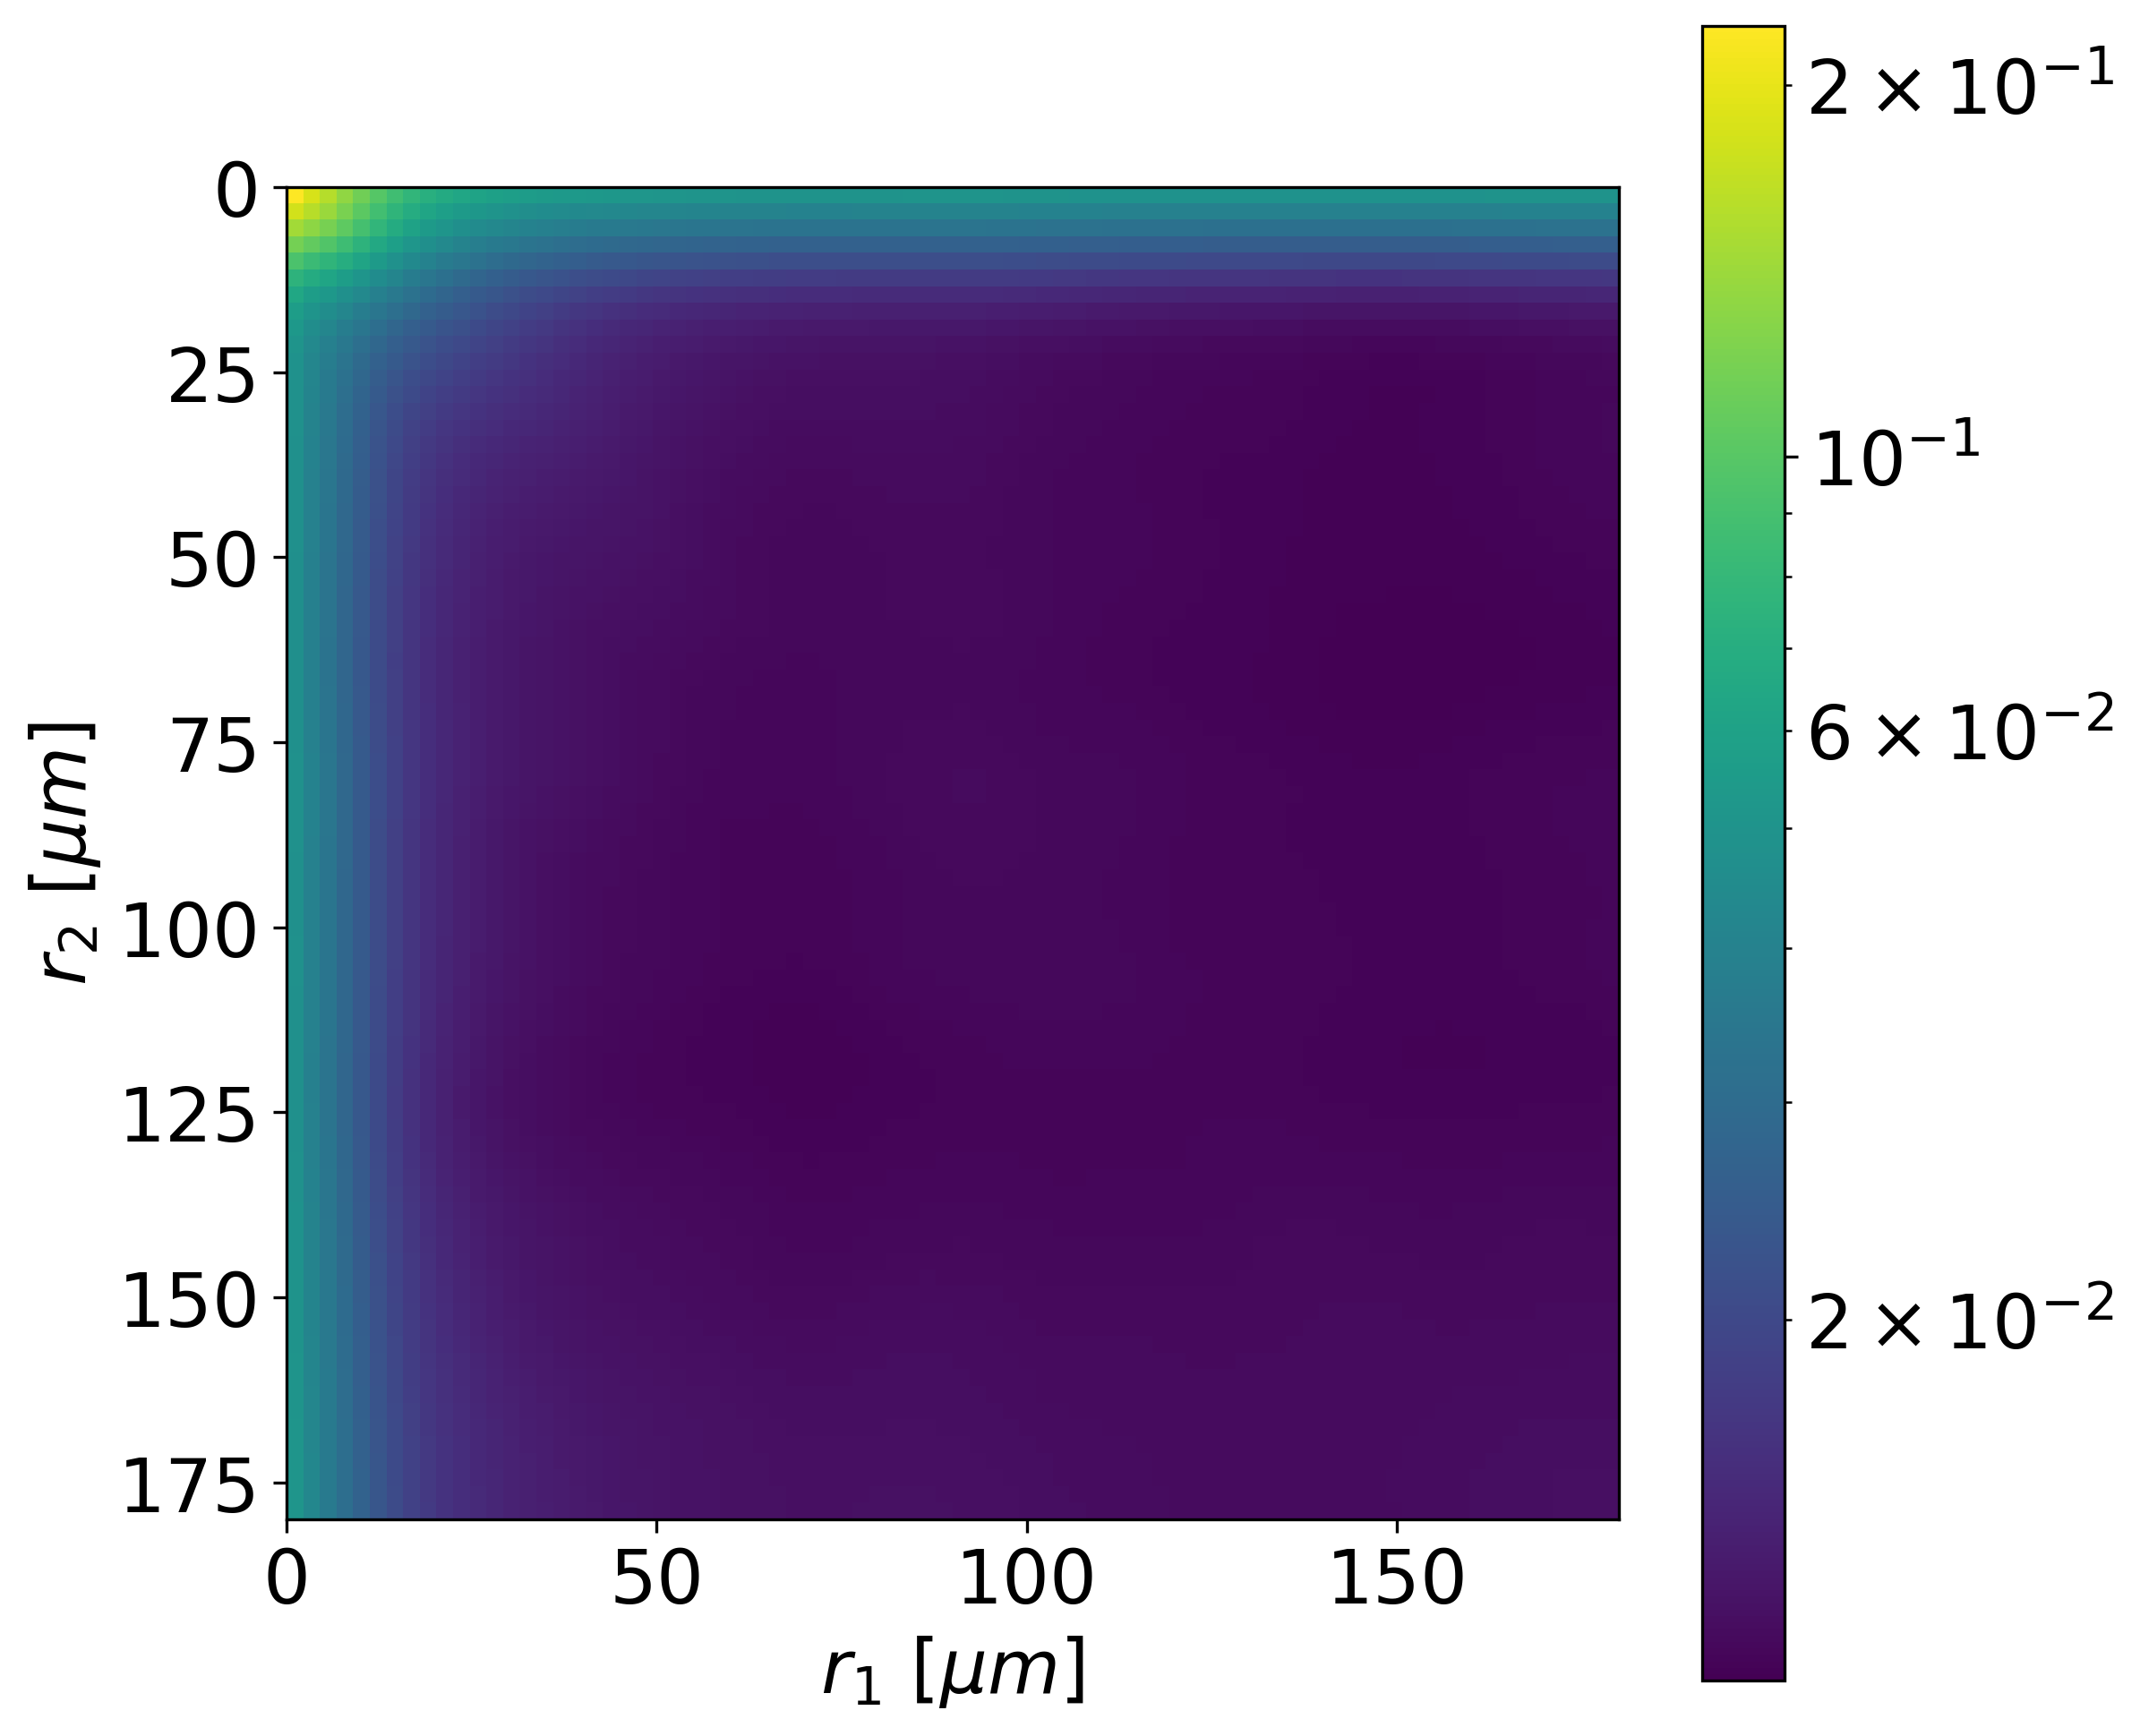
\includegraphics[width=0.4\linewidth]{images/shale-avg.png}
  \caption[]{Heatmaps of $S_3$ function for highly anisotropic samples. On the
    left: soil, on the right: shale. On the top: the function calculated for a
    rotation of the sample which aligns the direction of anisotropy with the
    axes, on the bottom: the function averaged across 100 random rotations.}
  \label{fig:heatmaps}
\end{figure*}

\begin{figure*}[tp]
  \centering
  \subfigure[$C_3$]{
    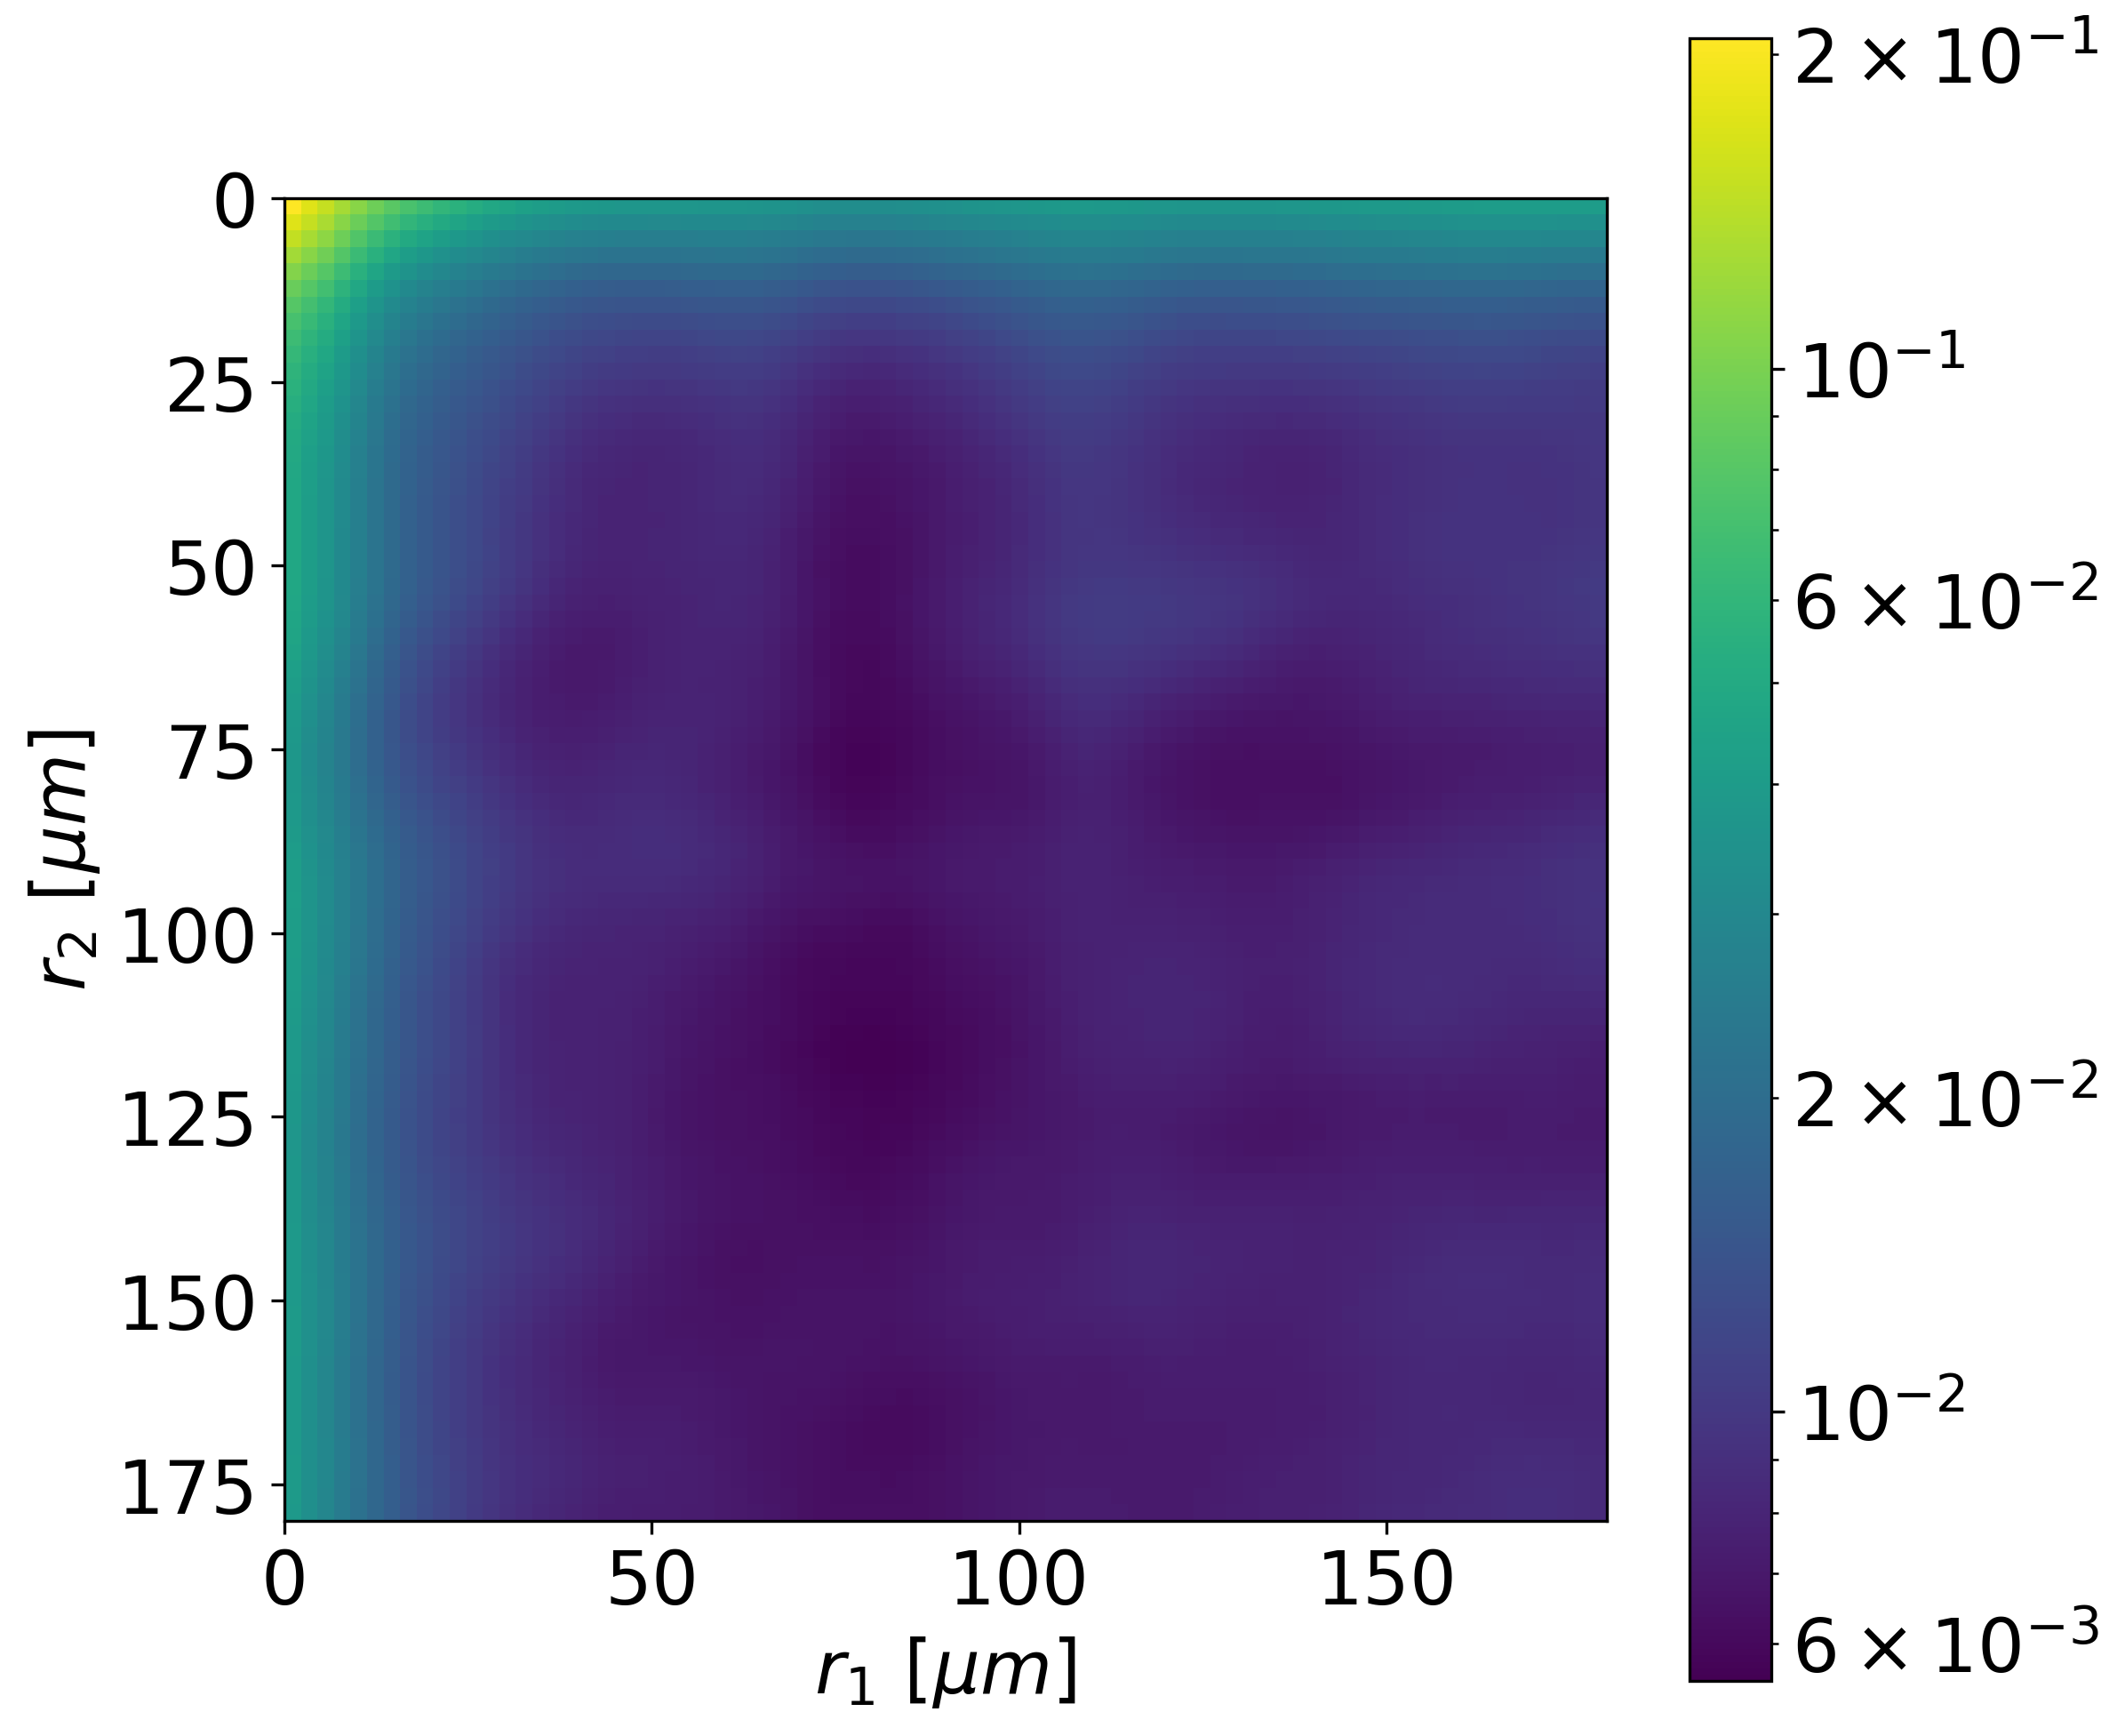
\includegraphics[width=0.4\linewidth]{images/c3-map.png}}
  \hfill
  \subfigure[$F_{sss}$]{
    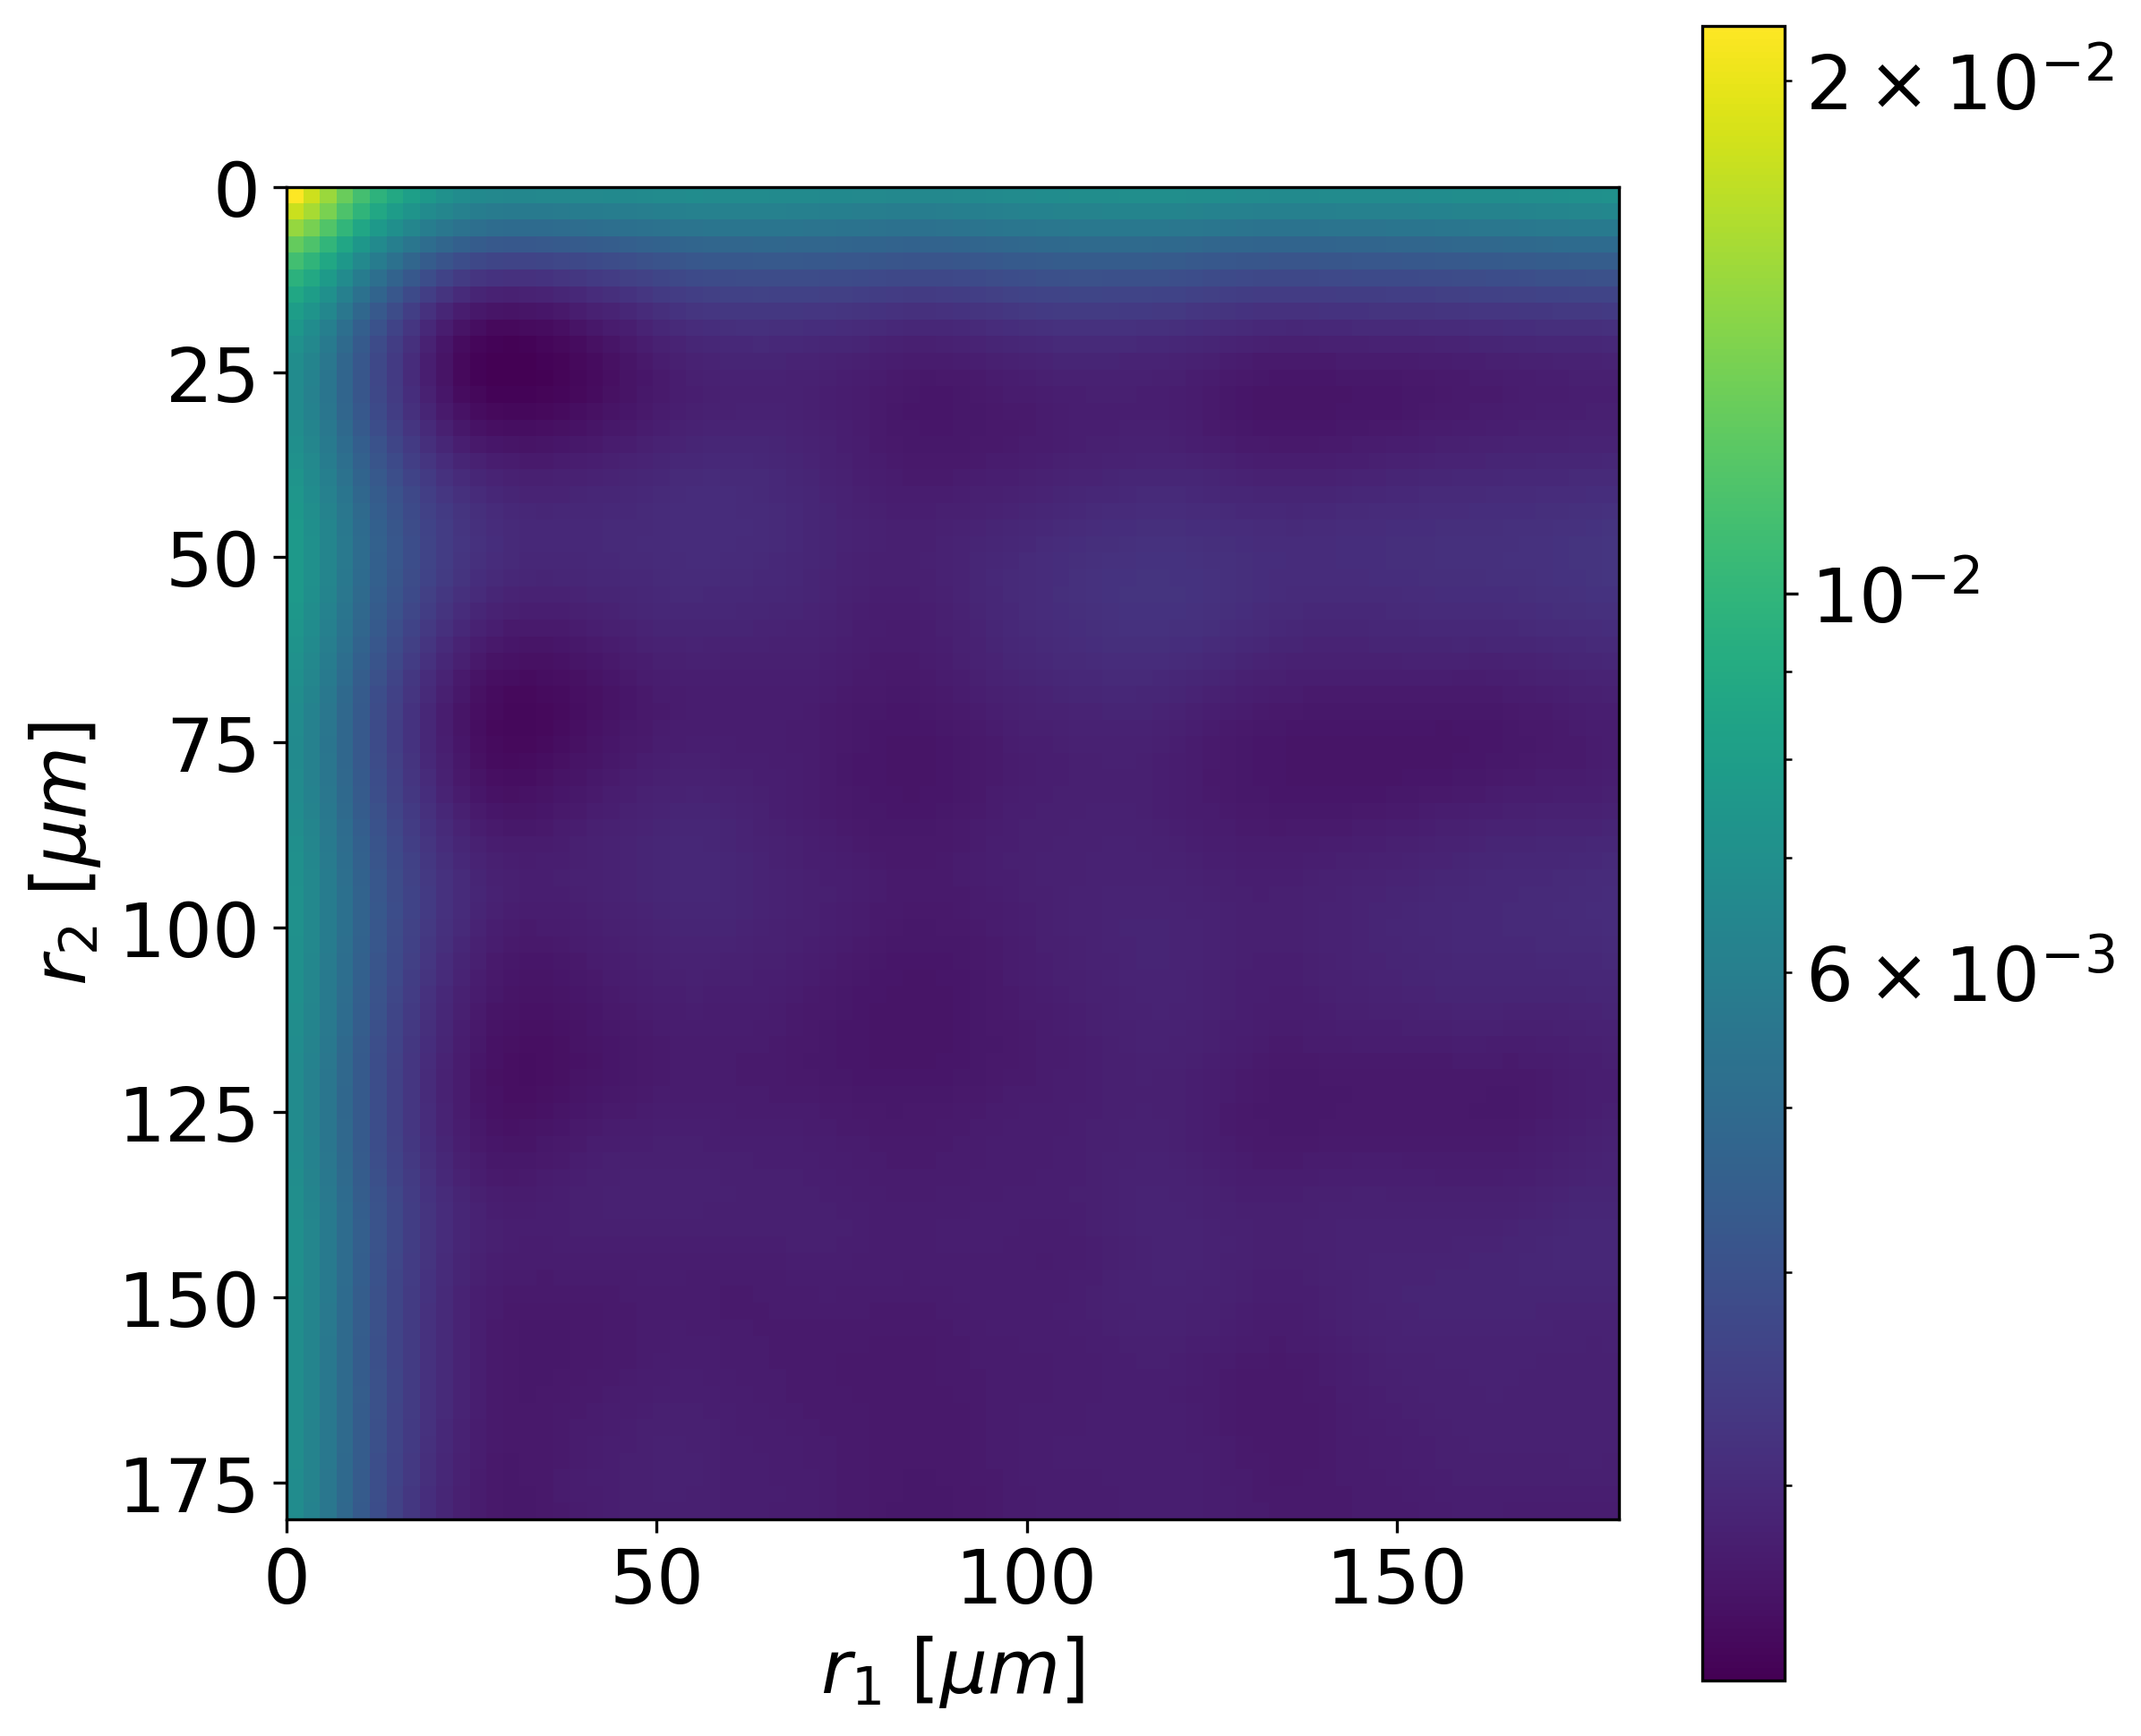
\includegraphics[width=0.4\linewidth]{images/surf3-map.png}}
  \vskip\baselineskip
  \subfigure[$F_{ssv}$]{
    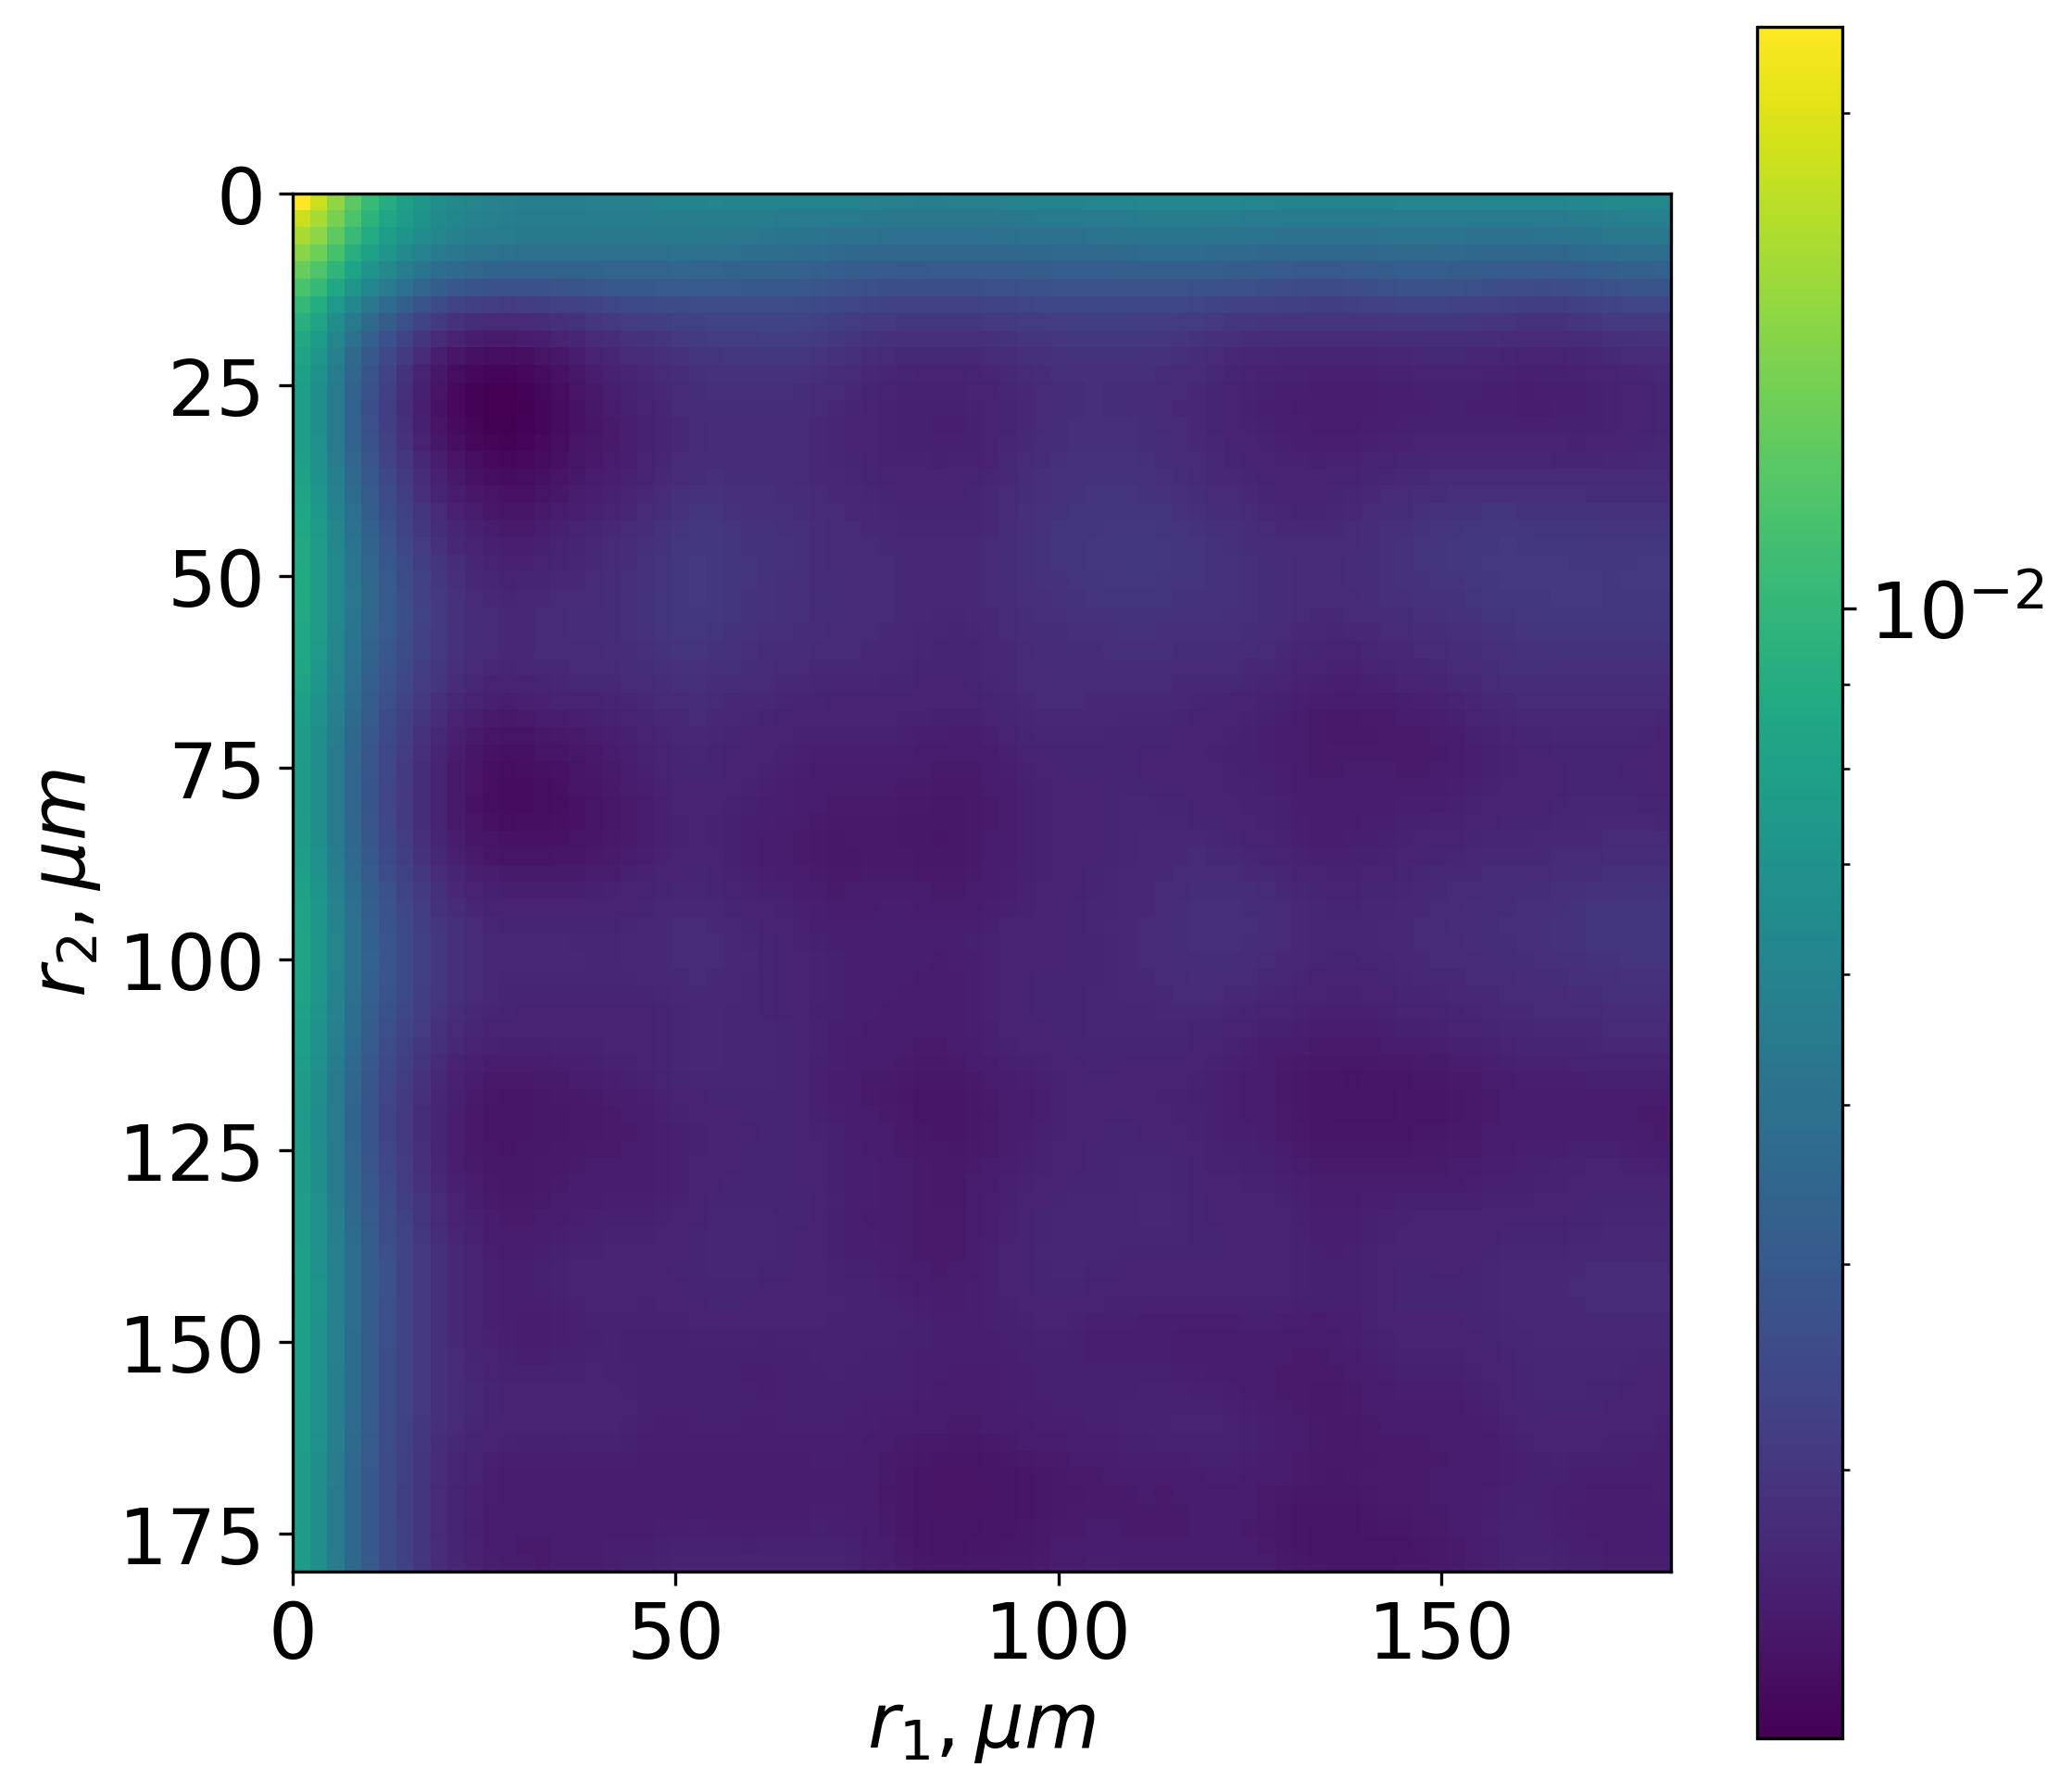
\includegraphics[width=0.4\linewidth]{images/surf2void-map.png}}
  \hfill
  \subfigure[$F_{svv}$]{
    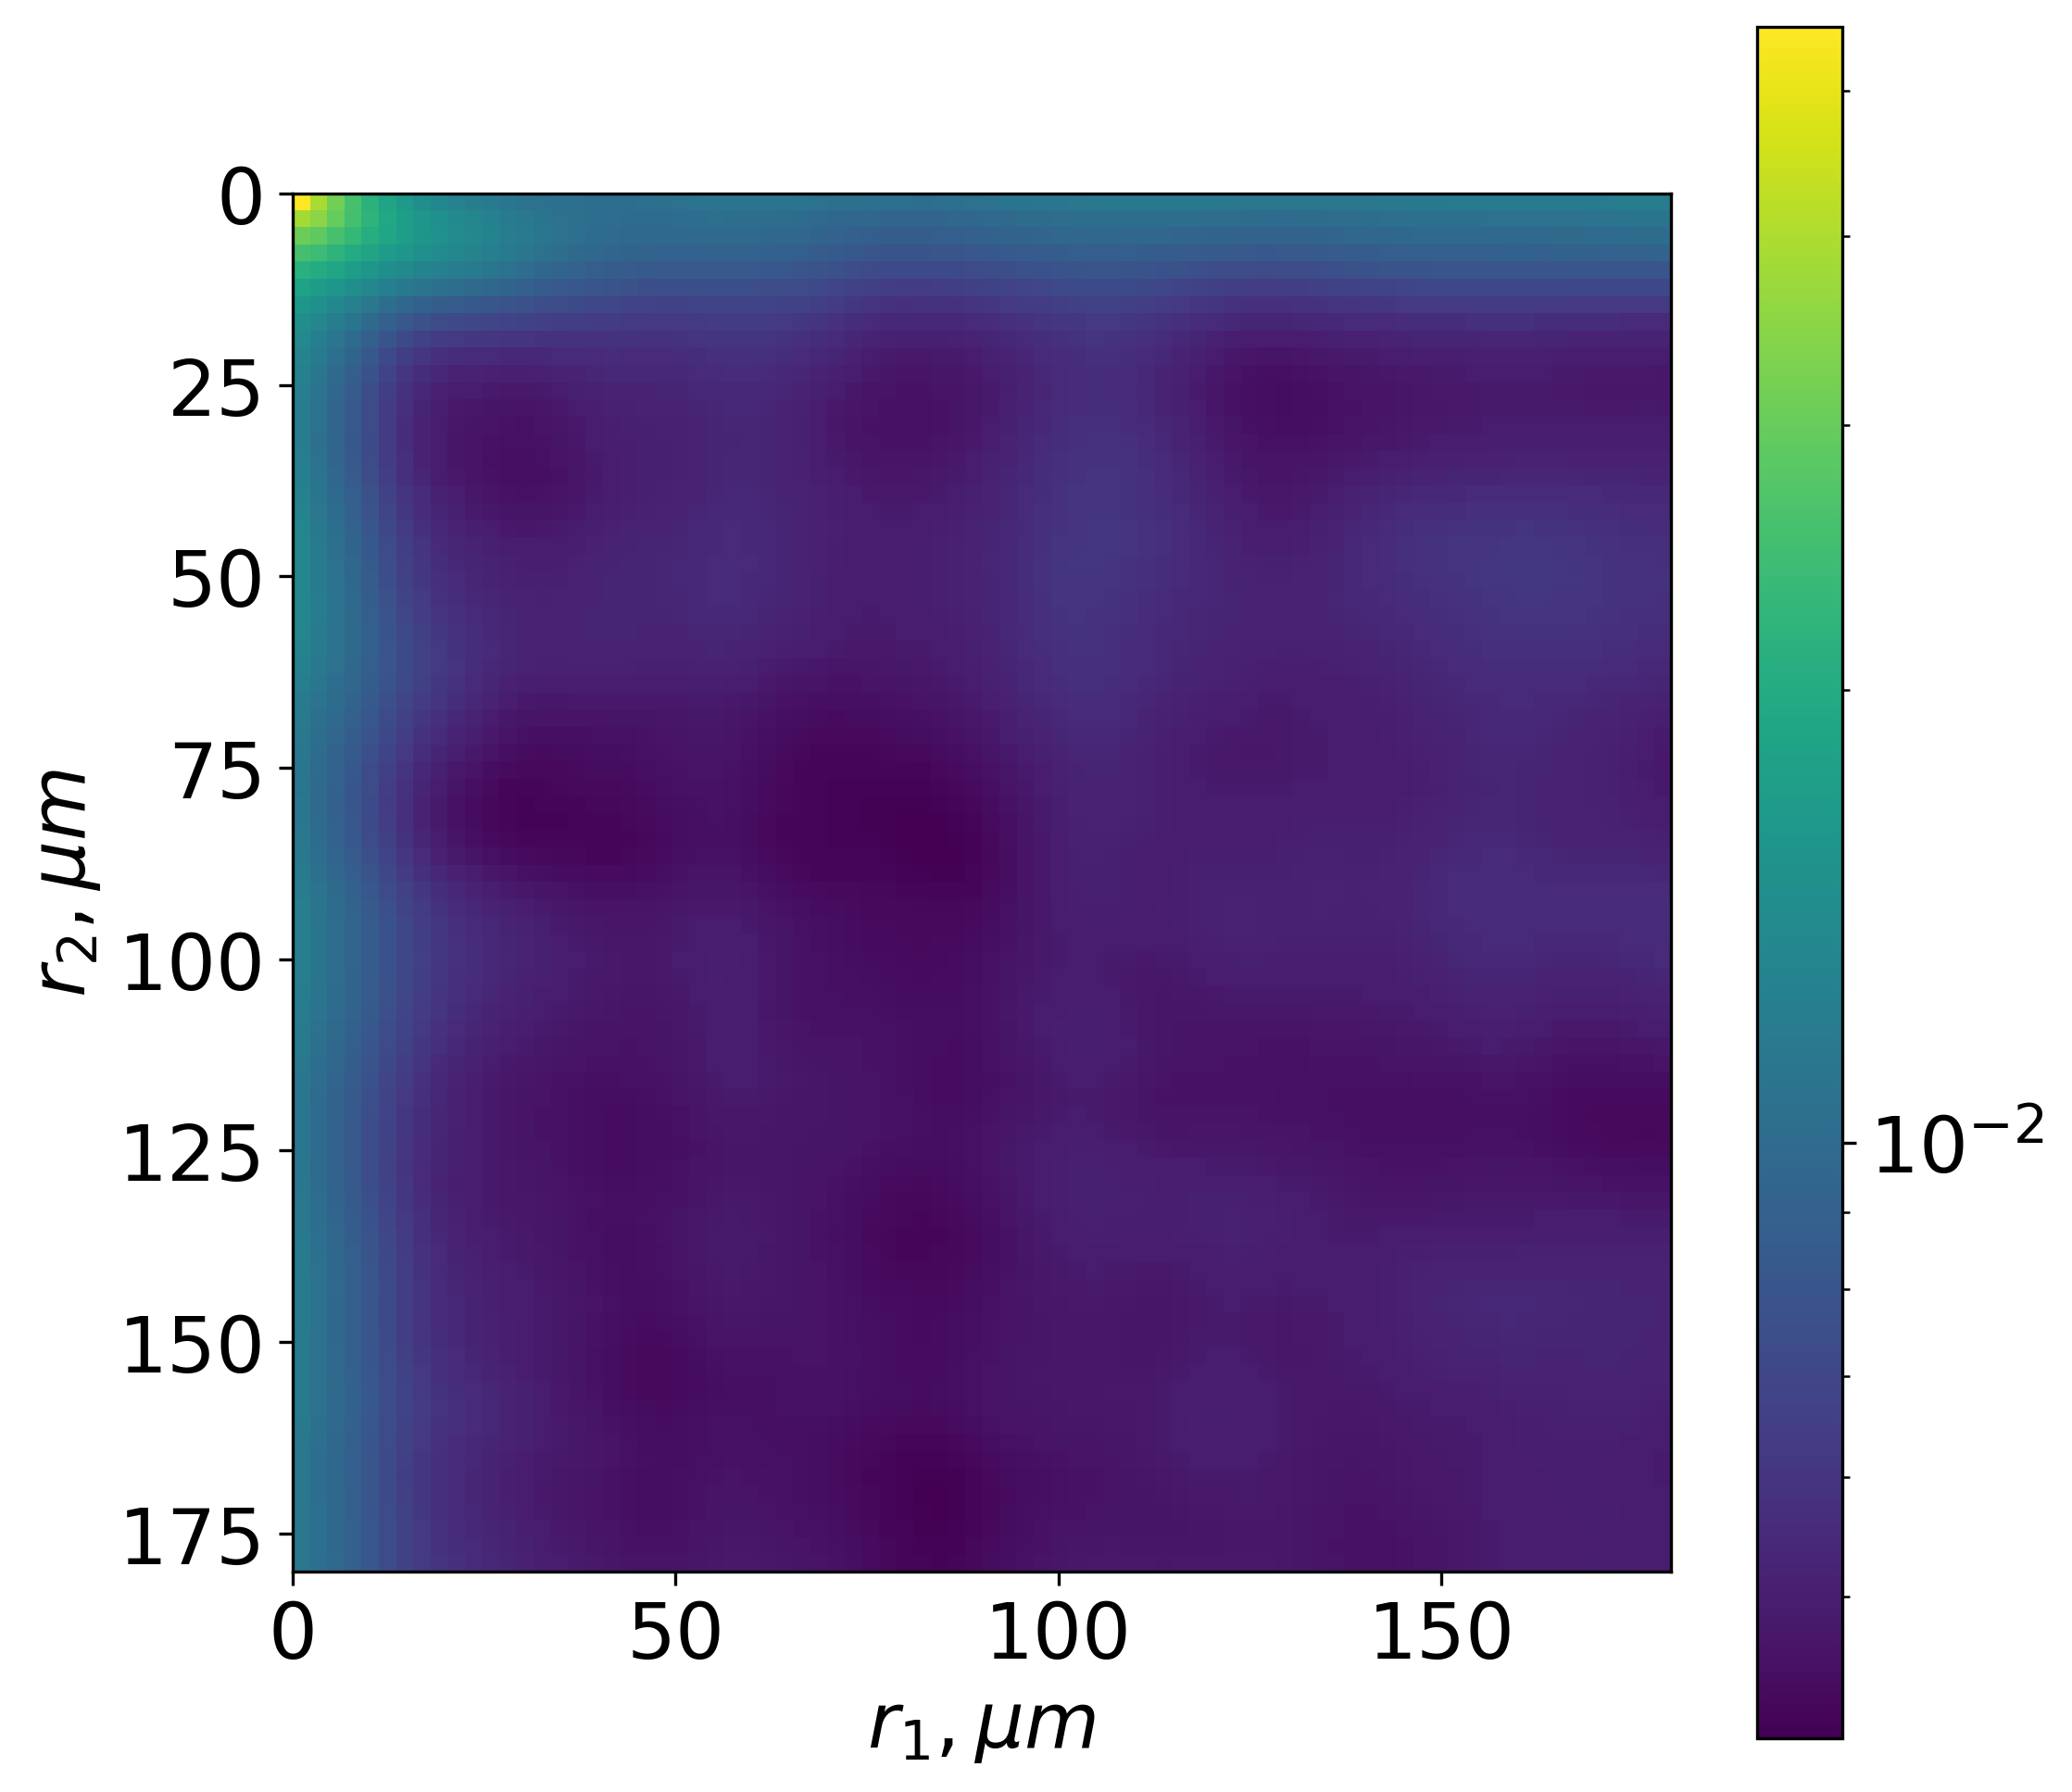
\includegraphics[width=0.4\linewidth]{images/surfvoid2-map.png}}
  \caption[]{Correlation maps for the sample of soil.}
  \label{fig:soil-maps}
\end{figure*}

\subsection{Execution times for our algorithms}
In this section we assess execution times of proposed computational algorithms
for random 3-dimensional arrays of bits (i.e. each element can be either 0 or
1). For ease of analysis, the arrays have the equal number of elements along
each direction therefore representing cubes of binary porous media. The number
of voxels $V$ in each cube increases from $1.25 \cdot 10^5$ to $2.7 \cdot 10^7$
linearly. Times of execution are measured separately for each function executed
on a CPU and a GPU. Hardware and software components used for testing are listed
in \cref{tab:machine}. Each computation of a correlation function is equivalent
to throwing of $V^{5/3}$ pattern triangles into the sample.
\begin{table*}[!htp]
  \centering
  \begin{tabular}{|c|c|}
    CPU & Intel Celeron 333 MHz \\
    RAM & 100500 GB DDR4 PC-XXXX \\
    GPU & AMD Navi 21 \\
    Julia & 1.10.0 \\
    CUDA.jl & 4.0
  \end{tabular}
  \caption{Parameters of the machine used to measure execution times of the
    algorithms described in this paper.}
  \label{tab:machine}
\end{table*}
\begin{figure*}[tp]
  \centering
  \subfigure[CPU]{
    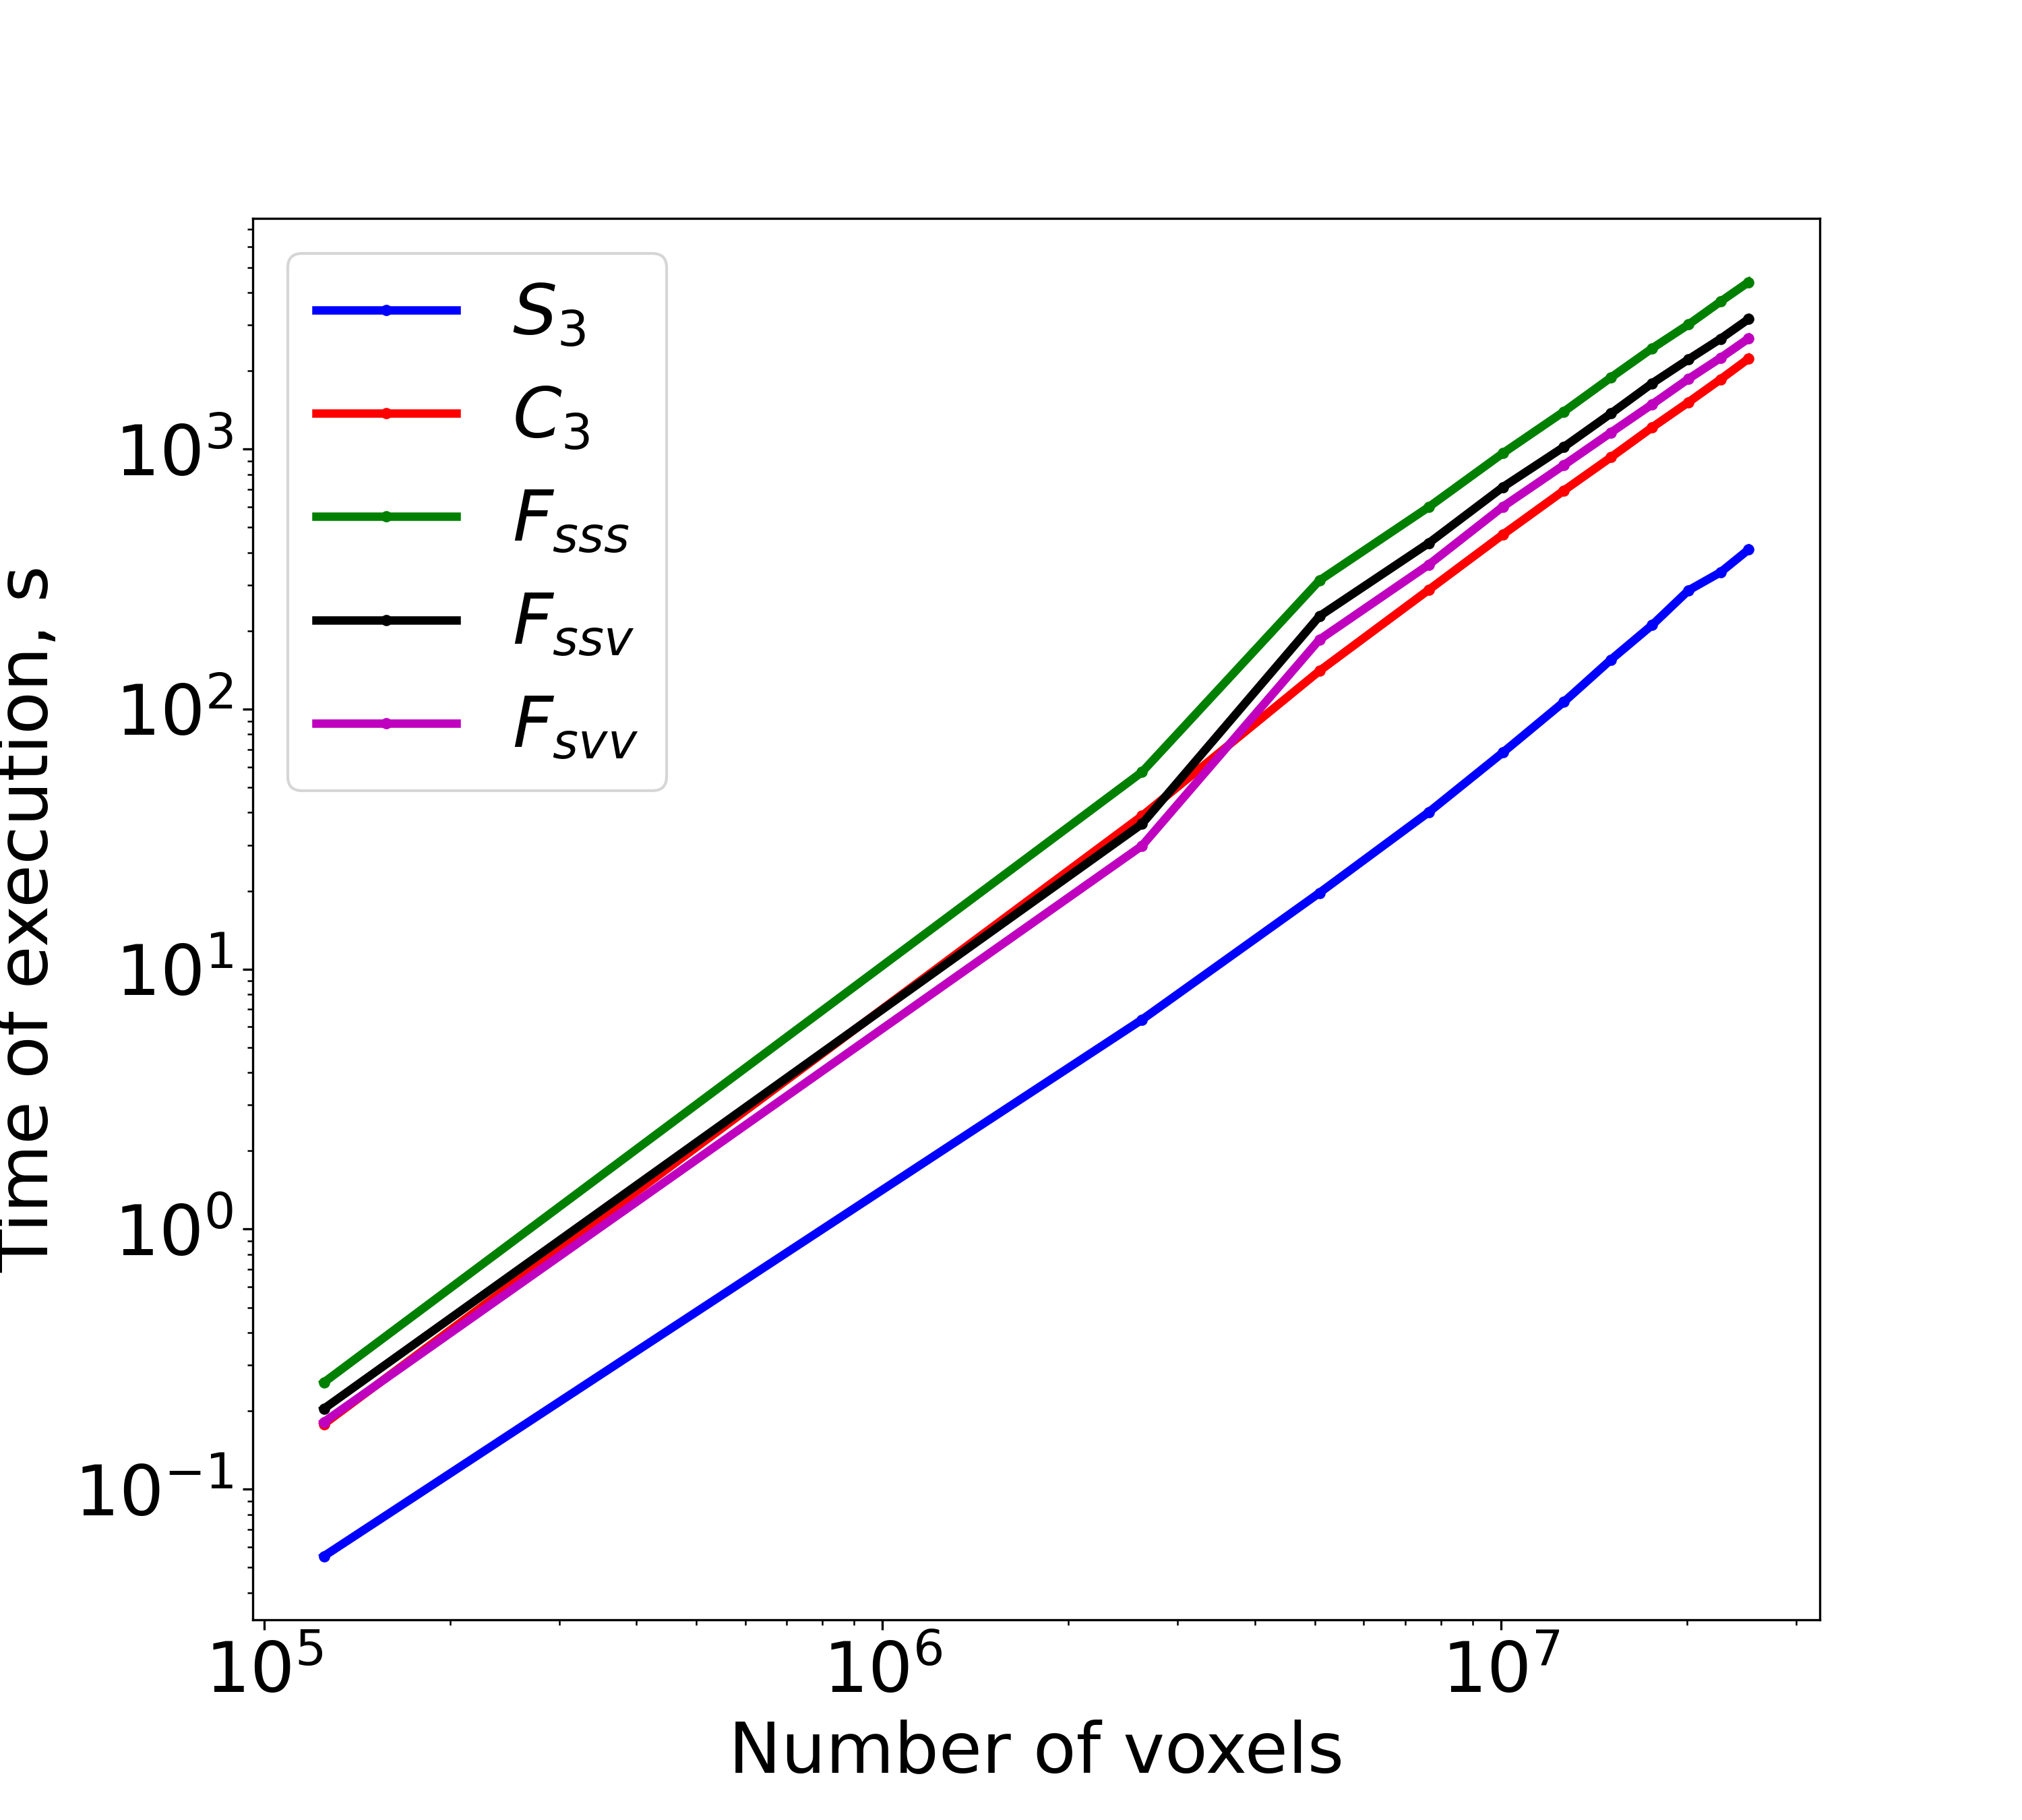
\includegraphics[width=0.4\linewidth]{images/timings-cpu.png}}
  \hfill
  \subfigure[GPU]{
    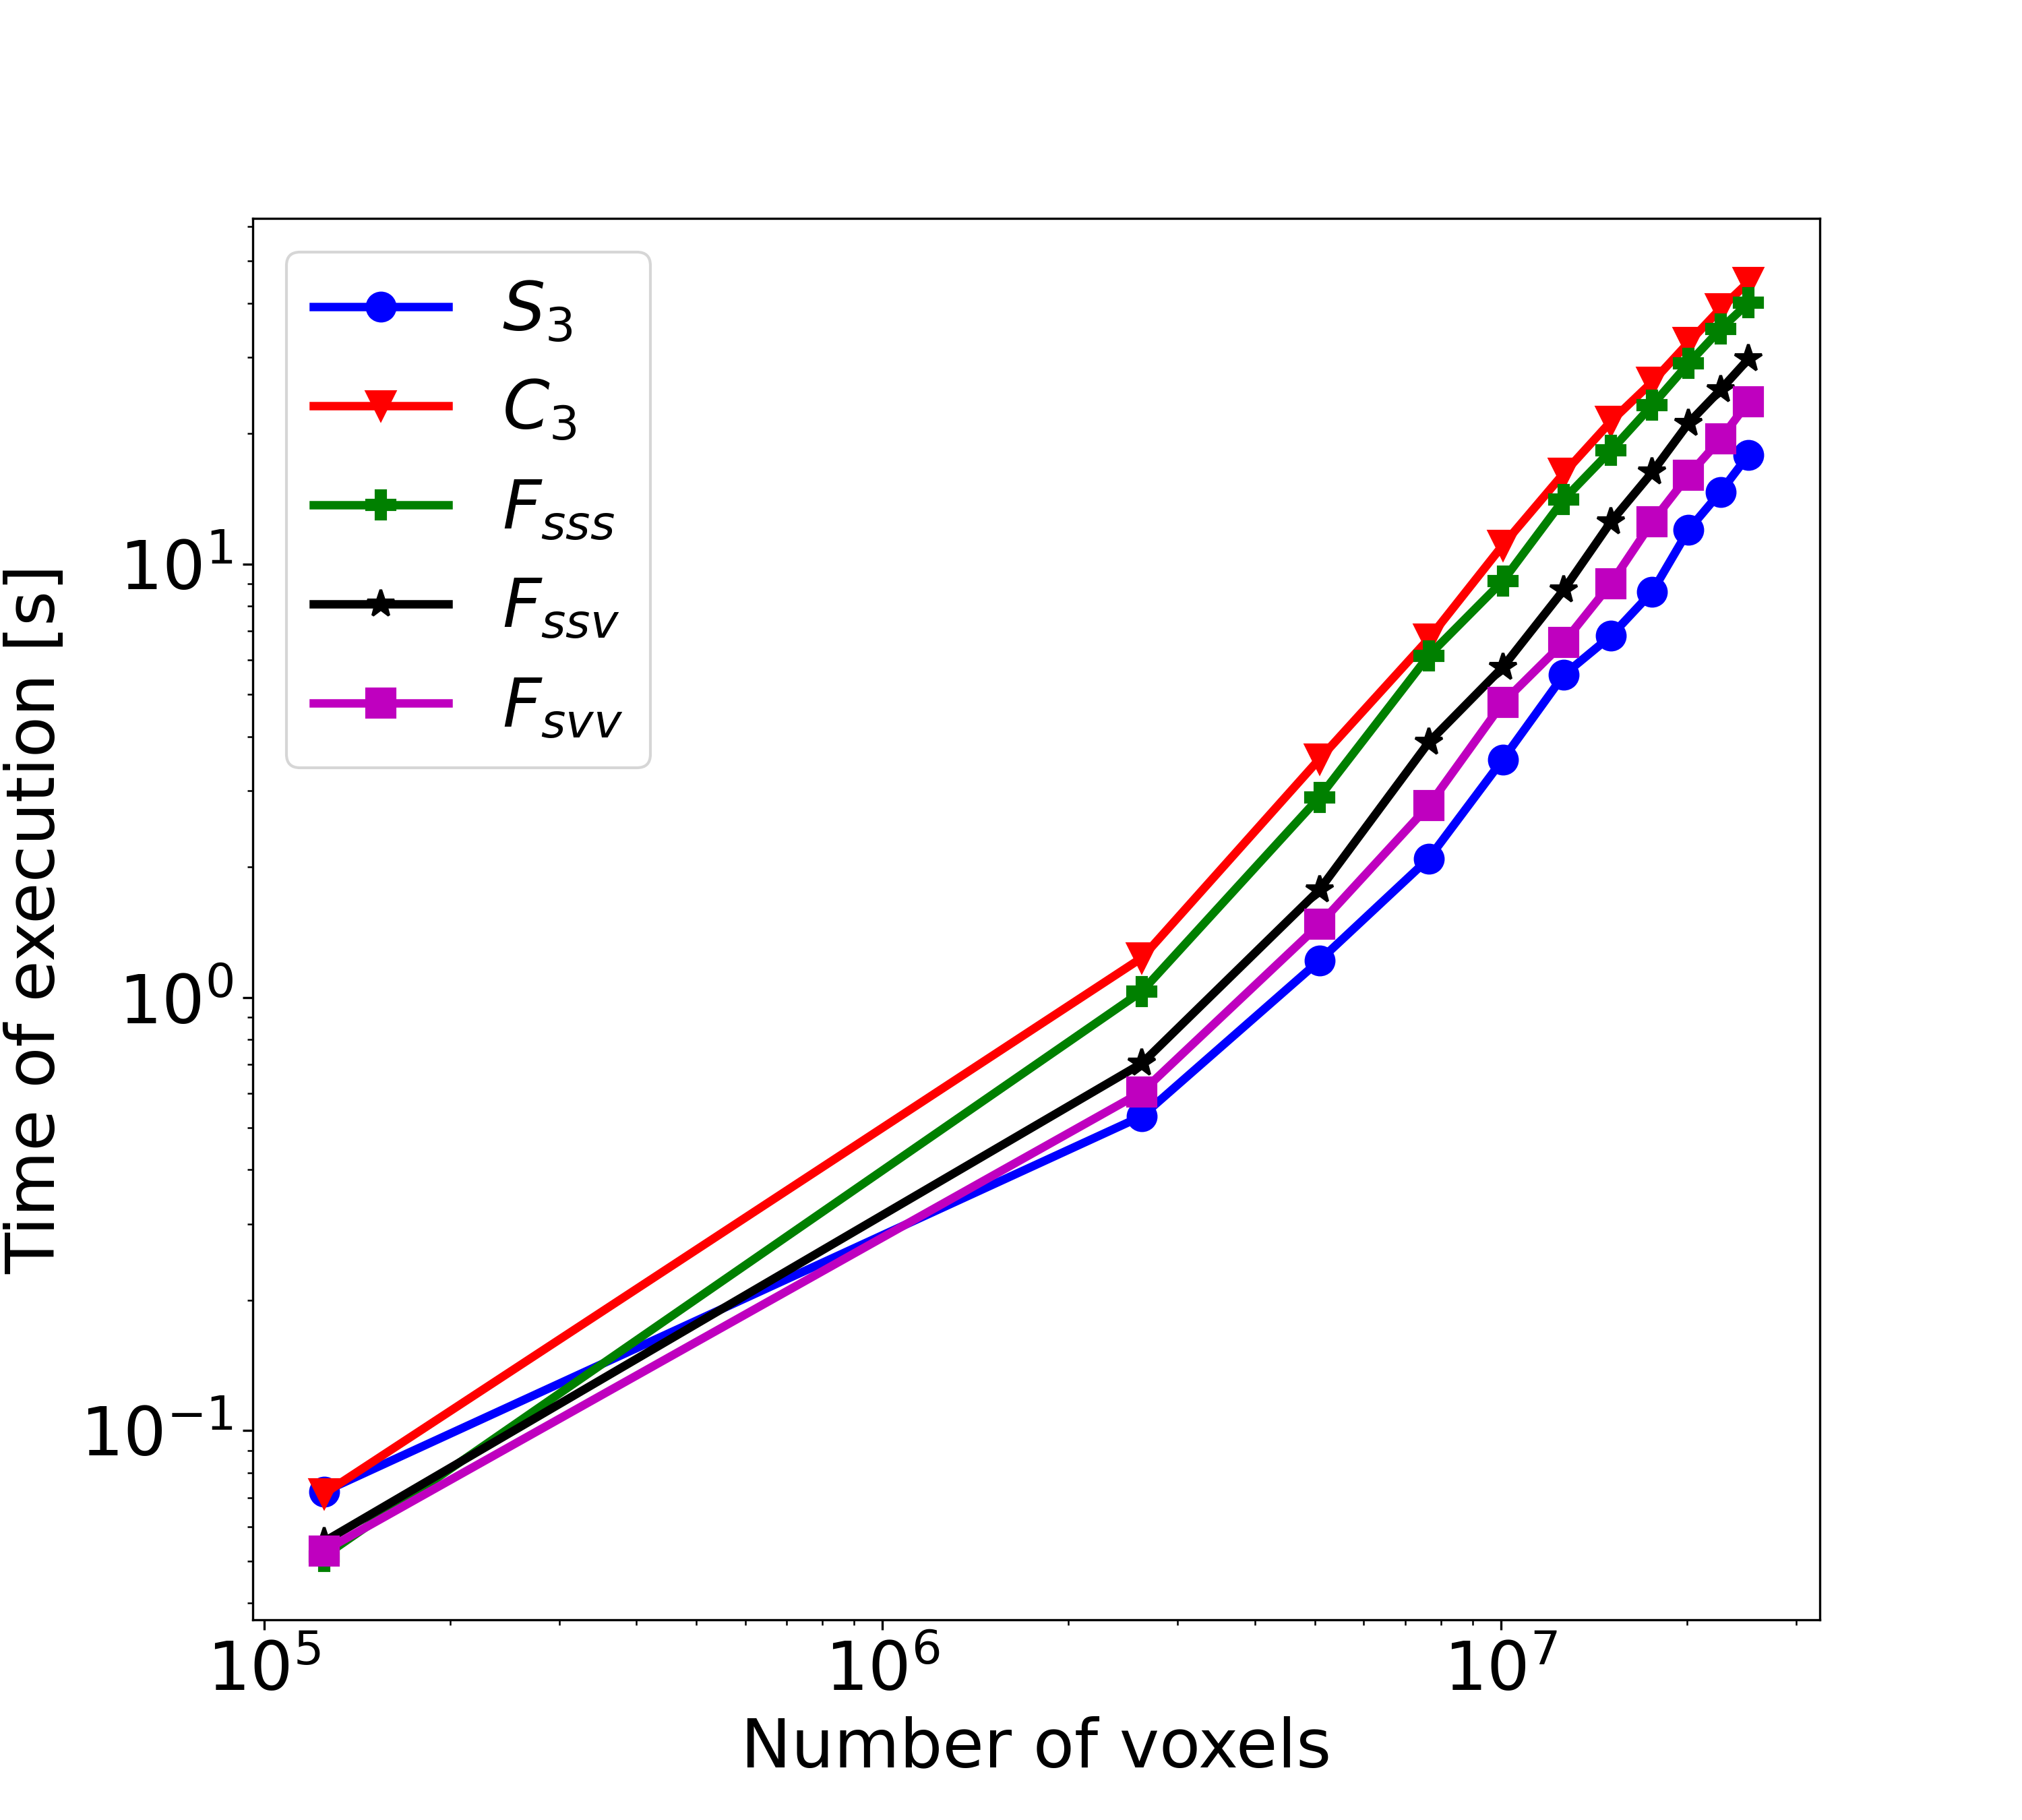
\includegraphics[width=0.4\linewidth]{images/timings-gpu.png}}
  \caption[]{Execution times of the algorithms proposed in this paper.}
  \label{fig:timings}
\end{figure*}

Wall times are shown in \cref{fig:timings}. It can be seen that the time of
execution is a power function of voxels number. GPU gives a
10x-100x performance boost depending on the correlation function. Note that
random pixel/voxel patterns are a hard test for some functions, especially for
$C_3$, as it produces a huge number of separate clusters. Thus, for real samples
execution times can be even smaller compared to those reported on \cref{fig:timings}.

Direct comparison against existing modern approaches, namely described by Malmir
et al. \cite{malmir2018} and by Sun et al. \cite{sun2022third}, is not always
straightforward due to algorithmic differences.  In particular, the latter cited
work computes 3-point correlation functions for sphere packings in the
continuous domain; however, on a GPU it takes approximately 28 hours to perform
$2\times10^6$ samplings (see Table 1 in \cite{sun2022third}).  Considering
verification results in \cref{sec:results}, it seems that it would be much
faster to discretize the sphere packing with appropriate $C_{0.5} > 0.97$ and to
utilize our package to assess correlation functions within tens of minutes
without any loss in accuracy.  For $S_3$ and 3-point surface functions, Malmir
et al. reported computation times of a couple of minutes for a $128^3$ voxels 3D
image with $2\times10^5$ samples on CPU (see section IV in \cite{malmir2018}).
In our case, we sample $\approx 31\times10^9$ triangles within 2 sec on CPU, and
less than a second on GPU.  Our implementation of $C_3$ is even more performant
compared to existing counterparts.

\section{Discussion}
\label{sec:discussion}
In this contribution we have presented two approaches to compute three-point correlation
function $S_3$ which is used as a basis to assess $C_3, F_{sss}, F_{ssv}$ and $F_{svv}$:
\begin{enumerate}
\item Computation in frequency domain using Fourier transform. This approach has
  computational complexity $O(n^2 \log n)$ and computes the whole correlation
  map. Unfortunately, it requires $O(n^2)$ additional memory and therefore can
  be used only with small inputs. Moreover, the whole Fourier image of the input
  is needed even if only a small portion of the correlation map is of interest.
\item Computation in spatial domain. This approach is implemented in
  \code{CorrelationFunctions.jl} package. This approach calculates the full map with
  complexity $O(n^3)$ but uses only $O(n)$ additional memory for shifted
  versions of the input. For our purposes the whole map is not needed and
  therefore the amount of calculations can be significantly reduced.
\end{enumerate}
It's tempting to create an algorithm which unites advantages of both approaches
(fast speed of the first and low memory consumption of the second) to
compute some desired slices of the full correlation map. It is known that Fourier
transform is the only linear transform which allows computation of convolution
in linear time. It is still an open question if there are linear transforms which
allow computation of convolution faster than a naïve approach
\cite{stone2008uniqueness,stone1998convolution}.

We have made execuation time comparisons of our algorithm with existing
algorithms.  However, it is also beneficial to compare some algorithmic details
against existing digital approaches -- proposed by Malmir~et~al
\cite{malmir2018} and another one by Smith and Torquato \cite{SMITH1988176}. The
first algorithm generates a triangle with fixed sides $r_1$ and $r_2$ and an
arbitrary angle $\theta$ between them and places it in the medium firstly making
a random translation and a rotation around a random vector by a random angle. By
making a large number of trials the algorithm gets a value of a three-point
correlation function at the point $(r_1, r_2, \theta)$. The second algorithm
takes a precalculated triangle $(r_1, r_2, \theta)$ from a web-like pattern and
places it in the medium without rotation, only applying a random
translation. This way the algorithm preserves orientation of triangles stored in
the pattern. The main advantage of our approach based on right triangle is in
its parallelizability and ease of implementation. A drawback is that an angle
between catheti of the sampling pattern is fixed to be $\theta = \frac{\pi}{2}$,
but can be mitigated by rotation of the pattern as a whole by an equivalent
operation of rotation of a sample. These rotations can be random as in the
Malmir et al. algorithm, or it can be a single rotation to align catheti of the
sampling triangle with the direction of anisotropy (\cref{fig:aniso}). The
latter allows computing directional 3-point correlation functions for
anisotropic structures similar to 2-point counterparts
\cite{10.1063/1.4867611,EPL1}.

As was mentioned in the \cref{sec:intro} section, computation of 3-point
correlation functions can be beneficial for some applications, yet the trade-off
between computational/storage burden due to higher orders and information
content is still not clear. The same goes for representation of the correlation
functions -- either in the form of averaged or directional functions, or as a
full correlation map. The latter is larger than the original image and was found
beneficial only in a limited number of applications, for example, in 3D
stochastic reconstructions from 2D cuts
\cite{cherkasov2021adaptive}. Computation of 3-point functions for 3D image even
along a single direction with a simplified pattern in the form of right-angle
triangle produces a 2D matrix similar in size to a 2D cut through the sample at
hand \cref{fig:workflow}. Averaging over a huge number of directions produces
the same volume of data, but looses all information about directional
differences within the structure. Computation of CFs with n > 3 results in
multidimensional matrices larger than the 3D image. The only way to keep this
profusion of floats at bay is to utilize the pattern that can be described with
a single parameter while shifting without rotations
\cite{chen2019hierarchical,chen2022}. In this fashion the results can be still
represented by a single function similar to 2-point CFs. But weather this
approach produces the descriptors with higher information content is an open
question.  In light of this discussion, at this point we decided to limit
\code{CorrelationFunctions.jl} with $n=3$, keeping in mind that extension of our
algorithms to $n>3$ for $S_n, C_n, F_{s...s}$ and $F_{s...v}$ is actually not
that complicated \cite{dimitrakopoulos2010high}.

We mentioned that classic set of correlation functions describes both the
geometry and topology of the structure at hand -- but this is to yet unknown
extent. With the advent of analytical methods \cite{cherkasov2023towards} to
assess information content of arbitrary descriptor for structure of any size, it
will be possible to choose the most useful set of correlation functions and
compare their information content against classical and other metrics. If
computationally effective methodology for information content assessment will be
developed, it should amend all aforementioned uncertainties and provide a clear
winner -- a plethora of different 2-point CFs or a less numerous set of
higher-order functions. Such long awaited answer would not be universal thought
and depends not only on descriptor's information content versus data volume
ratio, but also on its applicability to solve particular problems. For example,
it is well known that cluster $C_2$ function provides a lot of information in
addition to $S_2$ \cite{JiaoPNAS}, yet it's application in stochastic
reconstructions is very limited due to computational burden of cluster
relabeling during annealing \cite{PLoS_ONE}. Still, effective information
content assessment techniques will provide a possibility to account for such
additional application constraints.

As described in this paper, 3-point CFs computations can be immediately applied
in a great number of research applications, for example: 1) flow and transport
velocity fields analysis or any data with non-Gaussian signatures, 2) deep
learning for structural and physical properties (at least to observe the
differences between 2-point and 3-point based training datasets), 3) structure
taxonomy and categorization. In all these and numerous other potential cases the
ability to compute directional 3-point functions may be crucial. Notably, the
organization of the code functions for 3-point CFs computation is similar to
those previously developed for 2-point functions \cite{CFsjlpaper}, thus,
allowing computation of cross-correlation, i.e., one can compute 3-point CFs for
multiphase images (while binary structures were used in this paper for
simplicity).

\section{Summary}
In this paper, we have considered the problem of computing n-point correlation
functions, namely $S_n, C_n, F_{s...s}$ and $F_{s...v}$, for which
computationally efficient algorithms can be developed (including computations on
GPU). For $n=3$ we have developed code in Julia language to compute $S_3, C_3,
F_{sss}, F_{ssv}$ and $F_{svv}$ with a right-angle triangle pattern. This
pattern is much easier to vectorize and parallelize compared to previously used
random triangle or spider-web sampling patterns. Moreover, it allows to easily
implement computations of directional 3-point CFs. The execution times for the
same number of sample are orders of magnitude lower than existing published
counterparts. We showed that the volume of data produced get unwieldy very
easily, especially if computations are performed in frequency domain. For these
reasons until information content of different sets of correlation functions
with different "n-pointness" is not known, it is seemingly no much reason to
increase the number of points. Nonetheless, developed algorithms and code are
universal enough to be easily extendable to any $n$ (with increasing
computational and RAM burden). All results are available as part of open source
package \code{CorrelationFunctions.jl}, developed by our group and freely
available to the public with numerous Jupiter notebooks showing examples of
applications to assess 3-point correlation functions for 2D and 3D images.

\appendix
\section{Computation of number of trials for non-periodic mode}
\label{sec:number-of-trials}
If the displacement vectors $x_1, x_2: x_1 \perp x_2$ are parallel to two
distinct unit vectors $i=(1,0,0)$, $j=(0,1,0)$ or $k=(0,0,1)$ then the number of
trials for the input array having dimensions $D = (D_x, D_y, D_z)$ is the
following:
\begin{equation}
  \begin{aligned}
    & Norm(A, x_1, x_2) = \prod_k D'_k \\
    & D' = D - x_1 - x_2
  \end{aligned}
\end{equation}

\section{Edge detection filter}
\label{sec:filter}
For edge detection we use a kernel with the width 7 pixels with coefficients
inversely proportional to distance to acentral element of the kernel. The
central element is determined by a property that all elements of the kernel sum
to zero:
\begin{equation}
  E_k = S \left\{
  \begin{array}{ll}
    -\sum\limits_{\substack{l \\ l \ne 0}} E_l & \quad k = 0 \\
    1 / \rho(k, 0) & \quad \text{otherwise}
  \end{array}
  \right.
\end{equation}
For 3D case $S=172.96$ and for 2D case $S=30.46$ \cite{postnicov20232}.

\bibliography{paper}
\end{document}
